%; whizzy paragraph
%; whizzy-paragraph "^\\\\dancersection"
% -initex iniptex -latex platex -format platex -bibtex jbibtex -fmt fmt
% $B0J>e(B whizzytex $B$r;HMQ$9$k>l9g$N@_Dj!#(B

%     Tokyo Debian Meeting resources
%     Kansai Debian Meeting resources
%     Copyright (C) 2012 Junichi Uekawa
%     Copyright (C) 2012 Nobuhiro Iwamatsu
%     Copyright (C) 2012 Koichi Akabe

%     This program is free software; you can redistribute it and/or modify
%     it under the terms of the GNU General Public License as published by
%     the Free Software Foundation; either version 2 of the License, or
%     (at your option) any later version.

%     This program is distributed in the hope that it will be useful,
%     but WITHOUT ANY WARRANTY; without even the implied warranty of
%     MERCHANTABILITY or FITNESS FOR A PARTICULAR PURPOSE.  See the
%     GNU General Public License for more details.

%     You should have received a copy of the GNU General Public License
%     along with this program; if not, write to the Free Software
%     Foundation, Inc., 51 Franklin St, Fifth Floor, Boston, MA  02110-1301 USA

%  preview (shell-command (concat "evince " (replace-regexp-in-string "tex$" "pdf"(buffer-file-name)) "&"))
% $B2hA|%U%!%$%k$r=hM}$9$k$?$a$K$O(Bebb$B$rMxMQ$7$F(Bboundingbox$B$r:n@.!#(B
%(shell-command "cd image2012-natsu; ebb *.png")

% progress memo:
% 2013/12-2014/05$B$,%^!<%8BP>]!"4X@>$O(B2013/12-2014/05($B2>(B)
% $B%$%Y%s%HEy$G$J$$>l9g$OM}M3$r=q$/$3$H!#(B
% $BI,MW$JJQ99E@$O(B FIXME $B$G5-O?$7$F$$$^$9!#(B

%%$B$3$3$+$i%X%C%@3+;O!#(B

\documentclass[mingoth,a4paper]{jsarticle}
\usepackage{monthlyreport}
\usepackage{supertabular}
\usepackage{subfigure}
\renewcommand*\thesubfigure{}

\usepackage{comment}

% $B%k%S(B for 201312tokyo
\def\ruby#1#2{%
\leavevmode
\setbox0=\hbox{#1}\setbox1=\hbox{\tiny#2}%
\ifdim\wd0>\wd1 \dimen0=\wd0 \else \dimen0=\wd1 \fi
\hbox{\kanjiskip=\fill
\vbox{\hbox to \dimen0{\tiny \hfil#2\hfil}%
\nointerlineskip
\hbox to \dimen0{\hfil#1\hfil}}}}

% section $B$NBe$o$j$N4D6-(B -- $B2~D{$9$k!#(B
\renewcommand{\dancersection}[2]{%
\newpage
$B$"$s$I$-$e$a$s$F$C$I(B $B$G$S$"$s(B 2014$BG/2F9f(B
%
% top line
\vspace{0.1mm}\\
{\color{dancerdarkblue}\rule{\hsize}{2mm}}

%
% middle text
%
\begin{minipage}[t]{0.6\hsize}
\color{dancerdarkblue}
\vspace{1cm}
\section{#1}
\hfill{}#2\\
\end{minipage}
\begin{minipage}[t]{0.4\hsize}
\vspace{-2cm}
\hfill{}
\includegraphics[height=8cm]{image200502/openlogo-nd.eps}\\
\vspace{-5cm}
\end{minipage}
%
% bottom line
{\color{dancerlightblue}\rule{0.66\hsize}{2mm}}
%
\vspace{2cm}
}
% end of dancersection.

\begin{document}

\begin{titlepage}
\thispagestyle{empty}

\hspace*{-2.5cm}

\includegraphics{image2012-natsu/gudeb.eps}\\
\vspace*{0.1cm}

\vspace*{2cm}
\rotatebox{10}{\fontsize{32}{32} {\gt $BEl5~%(%j%"(B/$B4X@>#D#e#b#i#a#nJY6/2q(B}}

\vspace*{-1.5cm}
\hspace*{11cm}
\includegraphics[height=6cm]{image200502/openlogo-nd.eps}\\
\vspace*{0.1cm}
\hfill $B$"$s$I$-$e$a$s$F$C$I(B $B$G$S$"$s(B 2014$BG/2F9f(B 2014$BG/(B8$B7n(B12$BF|(B $B=iHGH/9T(B
\end{titlepage}

\newpage
\thispagestyle{empty}\mbox{}
\newpage

\setcounter{page}{1}
\begin{minipage}[]{0.2\hsize}
 \definecolor{titleback}{gray}{0.9}
 \colorbox{dancerlightblue}{\rotatebox{90}{\fontsize{80}{80}
{\gt \color{dancerdarkblue}$B%G%S%"%sJY6/2q(B} }}
\end{minipage}
\begin{minipage}[]{0.8\hsize}
\hrule
\vspace{1mm}
\hrule
\setcounter{tocdepth}{1}
{\small
\begin{multicols}{2}
  \tableofcontents
\end{multicols}
} %FIXME: does not fit in one column! $B$7$+$7FsCJ$K$9$k$H$"$^$jH~$7$/$J$$!)(B $B??$sCf$N$"$?$j$G>OHV9f$H%Z!<%8?t$NHV9f$,6a$/$K$"$k$N$,%P%i%s%9NI$/$J$$5$$,$9$k(B
\vspace{1mm}
\hrule
\vspace{3cm}

\end{minipage}

% FIXME: $BK\J8$rDI2C$9$k$3$H!#(B
%-------------------------------------------------------------------------------
\dancersection{Introduction}{$B>e@n(B $B=c0l(B, $B;32<(B $BB:Li(B}
%-------------------------------------------------------------------------------

\subsection{$BEl5~%(%j%"(BDebian$BJY6/2q(B}

 Debian$BJY6/2q$X$h$&$3$=!#$3$l$+$i(BDebian$B$N@$3&$K$"$7$rF'$_F~$l$k$H(B
 $B$$$&J}$b!"$9$G$K$I$C$W$j$H$D$+$C$F$$$k$H$$$&J}$b!"7n$K0l2s(BDebian$B$K$D$$(B
 $B$F8l$j$^$;$s$+!)(B

 Debian$BJY6/2q$NL\E*$O2<5-$G$9!#(B

\begin{itemize}
 \item \underline{Debian Developer} ($B3+H/<T(B)$B$N0i@.!#(B
 \item $BF|K\8l$G$N!V(B\underline{$B3+H/$K4X$9$k>pJs(B}$B!W$r@0M}$7$F$^$H$a!"%"%C%W%G!<%H$9$k!#(B
 \item \underline{$B>l(B}$B$NDs6!!#(B
 \begin{itemize}
  \item $BIaCJ$P$i$P$i$J>l=j$K$$$k?M!9$,(B face-to-face $B$G=P2q$($k>l$rDs6!(B
	$B$9$k!#(B
  \item Debian $B$N$?$a$K$J$k$3$H$r8l$k>l$rDs6!$9$k!#(B
  \item Debian$B$K$D$$$F8l$k>l$rDs6!$9$k!#(B
 \end{itemize}
\end{itemize}

 Debian$B$NJY6/2q$H$$$&$3$H$G5f6KE*$K$O;22C<TA40w$,(BDebian Package$B$r$,$j$,$j(B
 $B$H:n$k%9!<%Q!<%O%C%+!<$K$J$C$?;Q$rLQA[$7$F$$$^$9!#>pJs$N6&M-!&3hMQ$rDL$7(B
 $B$F(B Debian$B$N:#8e$NG=F0E*$JE83+$X$NEZBf$H$7$F!"!V>l!W$H$7$F$N6u4V$rDs6!$9(B
 $B$k$N$,L\E*$G$9!#(B

\subsection{$B4X@>(B Debian $BJY6/2q(B}

 $B4X@>(B Debian $BJY6/2q$O(BDebian GNU/Linux $B$N$5$^$6(B
 $B$^$J%H%T%C%/(B($B?7$7$$%Q%C%1!<%8!"(BDebian $BFCM-$N5!G=$N;EAH!"(BDebian $B3&7($G5/(B
 $B$3$C$?=PMh;v!"$J$I$J$I!K$K$D$$$FOC$79g$&2q$G$9!#(B

 $BL\E*$H$7$F<!$N;0$D$r9M$($F$$$^$9!#(B
 \begin{itemize}
  \item $B%a!<%j%s%0%j%9%H$d7G<(HD$G$O$J$/!"D>@\4i$r9g$o$;$k;v$G$N>pJs8r49$NB%?J(B
  \item $BDj4|E*$K=8$^$l$k>l=j(B
  \item $B;qNA$N:n@.(B
 \end{itemize}

 $B$=$l$G$O!"3Z$7$$0l;~$r$*3Z$7$_2<$5$$!#(B

%-------------------------------------------------------------------------------
% end of header
%-------------------------------------------------------------------------------

\clearpage
\newpage
%201312tokyo
%-------------------------------------------------------------------------------
\dancersection{Debian GNU/Hurd 2013}{$BLnEg(B $B5.1Q(B}
%-------------------------------------------------------------------------------
\index{debian-gnu-hurd}

\subsection{$B$O$8$a$K(B}

 2013$BG/(B5$B7n(B21$BF|$K!"(BDebian GNU/Hurd 2013$B$,%j%j!<%9$5$l$^$7$?(B\cite{news-release-hurd}$B!#(B
 $B:#2s$O!"$3$N(BDebian GNU/Hurd 2013$B$r(B
\begin{itemize}
\item $B%$%s%9%H!<%k$7$F$_$?$j!"(B
\item $B;n$7$?$j(B
\item $BD4$Y$?$j(B
\end{itemize}$B!!(B
$B$7$?;v$r=q$$$F$_$^$9!#(B

\subsection{$B%$%s%9%H!<%k$7$F$_$k(B}

 Debian GNU/Hurd 2013$B$N%$%s%9%H!<%k(BCD$B%$%a!<%8$O!"(BHurd$B%Y!<%9$N%M%C%H%o!<%/%$%s%9%H!<%k2DG=$J%$%a!<%8$K$J$C$F$$$^$9!#$3$3$G$O!"<B:]$K(BLinux$B$N(BKVM$B$r;H$$!"(BDebian GNU/Hurd 2013$B$r%$%s%9%H!<%k$7$FF0$+$7$F$_$^$9!#(B

$B!!$J$*!"(BDebian GNU/Hurd 2013$B$O!"(Bi386$B%"!<%-%F%/%A%c$,BP>]$G$9$,!"(BAMD64(64bit)$B4D6-$N(BKVM$B>e$G$=$N$^$^2?$iLdBj$J$/F0:n$7$^$9!#(B

\begin{description} 
\item [Step 1.] debian sid$B$rMQ0U$7!"2a5n$NEl5~%(%j%"(BDebian$BJY6/2q$N(BKDE$B3+H/4D6-$N;qNA(B\cite{kde-devel-debian}$B$r;29M$K!"(Bbr0$B%G%P%$%9$r%;%C%H%"%C%W$7$F$*$-!"%$%s%?!<%M%C%H$X%"%/%;%9$G$-$k4D6-$rMQ0U$7$F$*$-$^$9!#(B
\item [Step 2.] Debian GNU/Hurd 2013$B$N(BNETINST CD$B%$%a!<%8$rF~<j$7$^$9!#(B
\begin{commandline}
$ wget http://ftp.debian-ports.org/debian-cd/hurd-i386/current/debian-hurd-2013-i386-NETINST-1.iso
\end{commandline}
%$
\item [Step 3.] KVM$B$r;H$$!"%$%s%9%H!<%k$7$^$9!#%3%D$H$7$F!"%G%#%9%/(BI/O$B$O(BIDE$B!"%M%C%H%o!<%/%G%P%$%9$O(Be1000$B$rMxMQ$9$k$H$h$$$G$9!#(B
\begin{commandline}
$ sudo aptitude install libvirt-bin virtinst
$ sudo qemu-img create -f raw /var/lib/libvirt/images/debian-hurd0 7G
$ sudo virt-install --connect=qemu:///system -n debian-hurd0 --ram 512 \
  --cdrom /home/yours/debian-hurd-2013-i386-NETINST-1.iso \
  --disk /var/lib/libvirt/images/debian-hurd0,bus=ide,size=7,format=raw,cache=writeback \
  --bridge=br0,model=e1000 --vnc --hvm --accelerate
\end{commandline}
%$
$B$^$?!"%$%s%9%H!<%i$G?V$+$l$k<ALd$OI=(B\ref{tab:hurd-install-qa}$B$N$h$&$K$7$F$$$^$9!#(B
\begin{table}[ht]
\begin{center}
\begin{tabular}{|l|l|l|p{5cm}|}
\hline 
$B9`HV(B&$B9`L\L>(B&$BCM(B &$BHw9M(B\\ \hline \hline
1 & country & other$B"*(BAsia$B"*(BJapan & \\ \hline
2 & Configure locales & United States en\_US.UTF-8 & \\ \hline
3 & Configure the keyboard & $B$*$D$+$$$N%-!<%\!<%I$K$F(B & 106$B%-!<$OL5$$(B\\ \hline
4 & NetworkConfigure Manually & 192.168.0.2$BEy(B & $B$*;H$$$N4D6-$K$F(B \\ \hline
5 & Partition disk & "Guided - use entire disk"	& $B4J0WE*$K$3$A$i$rA*Br!#(B\\ \hline
6 & mirror country & Japan$B;XDj$N!"(Bftp.jp.debian.org$B$rA*Br(B & \\ \hline
\end{tabular}
\end{center}
\caption{$B%$%s%9%H!<%i$G$N<ALd$X$N2sEzNc(B}
\label{tab:hurd-install-qa}
\end{table}

$B$J$*!"%$%s%9%H!<%kCf(B''Select and install software''$B%a%K%e!<$G!"(B
``Debian desktop environment''$B$r;XDj$7$F$$$k$H!"%$%s%9%H!<%i$,ESCf$G0[>o=*N;$7$F$7$^$$$^$9!#$=$N;~$OD|$a$F!"0lC6(B''Debian desktop environment''$B$r%$%s%9%H!<%k8uJd$+$i30$7$F$_$F!"(BStep 3.$B$+$i$d$jD>$7$H$J$j$^$9!#(B\footnote{$B<+J,$,$d$C$?;~$O!"(Bxserver-xorg-video-all$B$N%Q%C%1!<%80MB84X78$,K~$?$;$J$+$C$?MM$G$9!#:#$O<#$C$F$$$k$+$b$7$l$^$;$s!#(B}
\item [Step 4.] $B%$%s%9%H!<%k$,40N;$9$k$H!">!<j$K%V!<%H$7$F(Bvirt-viewer$B$K$F(BGNU/Hurd$B$,N)$A>e$,$j!"(B''login:''$B%W%m%s%W%H$,=P$^$9$N$G!"%m%0%$%s$9$k$H;H$($^$9!#(B
\end{description}

\subsection{$B;H$&$K$"$?$C$F$A$g$C$HCN$k$HNI$$$3$H(B}

 $B4pK\E*$K$O(BUNIX$B7O%7%9%F%`$N;H$$>!<j$G$9!#(BDebian GNU/Linux$B;H$($kJ}$J$i!"Hs>o$K$H$C$D$-0W$$46$8$G$9!#$b$A$m$s$G$9$,!"(BDebian$B$J$N$G!"(Bdpkg/apt$B$O$=$N$^$^;H$($^$9!#(B

 $B$?$@!"(Bhurd$B$r;H$&$K$"$?$C$F!"$$$/$D$+(BLinux$B$H$O0c$&E@$,$"$k$N$G!"CN$k$HJXMx$J7o$r$$$/$D$+0J2<$K5-:\$7$^$9!#(B

\begin{enumerate}
\item $B%7%9%F%`Dd;_(B \\
Linux$B%7%9%F%`$G$9$H!"(B/sbin/shutdown$B!!(B-h now $B$H$+!"(BCTL+ALT+DEL$B$N%-!<%"%/%7%g%s$H$+$,0lHLE*$+$H;W$$$^$9$,!"(Bhurd$B$N>l9g$O(B sync;halt$B$H$J$j$^$9!#(Bshutdown$B$r(Bhurd$B$GMxMQ$9$k$H2r$k$N$G$9$,!"(Binit$B$HO"7H$G$-$J$/$F(Bshutdown$B%3%^%s%I$,ESCf$G<:GT$7$^$9!#(B
\item $B%M%C%H%o!<%/4X78$N@_Dj(B \\
Linux$B%7%9%F%`$G$9$H!"(Bip$B%3%^%s%I$H$+!"(Bifconfig$B%3%^%s%I$H$+$"$j$^$9$,!"(B
hurd$B$G$9$H(Bsettrans$B%3%^%s%I;H$C$F!"(B/hurd/$B%G%#%l%/%H%j0J2<$N%M%C%H%o!<%/MQ$N(Btranslator$B$H$$$&%3%^%s%I72$H!"FCDj$N%G%P%$%9%U%!%$%k$r7k$S$D$1$k$H$$$&;v$GBP1~$7$^$9!#(B
\begin{commandline}
NIC$B@_Dj$NNc(B:
# settrans -fgcap /servers/socket/2 /hurd/pfinet -i eth0 \
     -a 192.168.0.5 -m 255.255.255.0 -g 192.168.0.1
\end{commandline}
 $B$^$?!"(Bhurd$B$N>l9g!"(Btranslator$B$X(Bfsysopts$B%3%^%s%I$G;X<($r=P$9$3$H$K$h$j!"(Btranslator$B$,BP1~$7$F$$$l$P@_DjJQ99$b$G$-$^$9!#(B
\begin{commandline}
NIC$B$N@_Dj$,$I$&$J$C$F$$$k$+!)(B
# fsysopts /servers/socket/2
/hurd/pfinet --interface=/dev/eth0 --address=10.3.0.1 --netmask=255.255.0.0 --gateway=10.3.0.128
(ps -auxww | fgrep pfinet$B$H$+$7$F$b2D!K(B
NIC$B@_DjJQ99$NNc(B:
# fsysopts /server/socket/2 -a 10.3.0.2 -m 255.255.0.0 -g 10.3.0.128 
\end{commandline}
\item $B%U%!%$%k%7%9%F%`$N%^%&%s%H(B\\
Linux$B$@$H(Bmount$B%3%^%s%I$G$9$,!"(Bhurd$B$N>l9g$G$9$H!"(B
\begin{commandline}
$BJ*M}%G%P%$%9$r%^%&%s%H(B
# settrans /mnt /hurd/ext2fs /dev/hd0s5
CD$B%$%a!<%8$r%^%&%s%H(B
# settrans /mount/point /hurd/iso9660fs CD_image.iso
NFS$B$r%^%&%s%H(B
# settrans -cgap /mount/point /hurd/nfs 192.168.1.1:/home
\end{commandline}
$B$H$$$&7A$G!"%U%!%$%k%7%9%F%`MQ$N(Btranslator$B$r(Bsettrans$B%3%^%s%I$G%^%&%s%H%]%$%s%H$K7k$S$D$1$F$7$^$&$H$$$&<j$r;H$$$^$9!#(B
\end{enumerate}

 $B$=$NB>$K$D$$$F$O!"(BDebian GNU/Hurd Configuration(\url{http://www.debian.org/ports/hurd/hurd-install})$B$r8+$k$HNI$$$G$9!#(B

\subsection{X$B$rF0$+$7$F$_$k(B}

$B!!%m%0%$%s$7$F$=$N$^$^(BCUI$B$GMxMQ$H$$$&(B\ruby{$B4A(B}{$B$*$H$3(B}$B$J;H$$J}$b3N$+$K$G$-$^$9$,!"(BX$B$0$i$$$OF0$+$7$?$$>l9g$b$"$k$o$1$G$9!#;n$7$KF0$+$7$F$_$^$9!#(B

\begin{commandline}
# aptitude install xserver-xorg-video-cirrus xinit fluxbox
# xinit
$B$3$3$G!"Gr$$%&%#%s%I%&$,=P$k$N$G!"$=$N%&%$%s%I%&$K%+!<%=%k$r9g$o$;!"(B
# fluxbox &
\end{commandline}

 $B47$l$F$-$?$i!"(B/root/.xinitrc$B$H$+$K$$$m$$$m=q$/$HJXMx$G$9!#(B

 $B$J$*!":#2s(BX$B$r(Broot$B$GF0$+$7$F$$$^$9!#K\Mh!"0lHL%f!<%6$GF0$+$;$k$HNI$$$N$G$9$,!"(B
$B<+J,$O$^$@$7$C$+$jD4$Y$-$l$F$$$^$;$s!#(B

\subsection{GNU Hurd$B?^2r(B}

  GNU Hurd$B$r?^2r$7$F$_$^$9!#(B

\begin{figure}[H]
\begin{center}
 \includegraphics[scale=0.3]{image201312/gnu-hurd-schema.eps}
 \caption{OS$B$N?^2r(B}\label{fig:gnu-hurd-schema}
\end{center}
\end{figure}

 $B?^$N$H$*$j!"(B

\begin{itemize}
\item $B%+!<%M%kK\BN$O(Bmach-1.3/1.4
\item $B%U%!%$%k%7%9%F%`!"%M%C%H%o!<%/%$%s%?!<%U%'!<%9$J$I$O(B/hurd/$B0J2<$K$"$k(Btranslator$B$H8F$P$l$k<B9T%P%$%J%j$K$h$k%f!<%6%W%m%;%9(B
\item $B%+!<%M%kK\BN$H(Btranslator$B72$O<g$K(BMIG$B$H8F$P$l$k(BRPC$B$J$I$GDL?.(B
\end{itemize}

$B$H$$$&9=B$$K$J$C$F$$$^$9!#(B

\subsection{$B=*$o$j$K(B}

 Debian GNU/Hurd $B$O!"$^$@$$$m$$$m$HL$3+Bs$JItJ,$bB?$$$G$9!#$^$?!"(B
gnu hurd$BK\BN$b$$$m$$$m$HB>$K5!G=$,I,MW$J>uBV$G$9!#(B

 $B$9$G$K$$$m$$$m$H40@.$5$l$?(BDebian GNU/Linux$B$bLLGr$$$G$9$,!"(B
$B$$$m$$$mL$40@.$J(BDebian GNU/Hurd$B$b(BHack$B$7$FM7$V$K$OLLGr$$$H(B
$B;W$$$^$9!#3'MM$b$<$R!#(B

\begin{thebibliography}{0}
  \bibitem{news-release-hurd}
    {\footnotesize{
       Debian.org,``Debian GNU/Hurd 2013 $B%j%j!<%9(B!'',
       \url{http://www.debian.org/ports/hurd/hurd-news}
       }}
  \bibitem{kde-devel-debian}
    {\footnotesize{
       $BLnEg(B $B5.1Q(B,$B!V(BDebian$B3+H/<T$N(BKDE$B4D6-$"$l$3$l!W(B,$BBh(B85$B2sEl5~%(%j%"(BDebian$BJY6/2q;qNA(B,
       \url{http://tokyodebian.alioth.debian.org/pdf/debianmeetingresume201202.pdf}
       }}
\end{thebibliography}

%201401 tokyo
%-------------------------------------------------------------------------------
\dancersection{Debian Pure Blend}{$BLnEg(B $B5.1Q(B}
%-------------------------------------------------------------------------------
\index{debian-pure-blends}

\subsection{Debian Pure Blend}

 Debian$B$KMQ0U$5$l$F$$$kBgNL$N%Q%C%1!<%8$r$&$^$/;H$$!"$=$N$^$^$N(BDebian$B$N%j%]%8%H%j$rMQ$$$k;v$G!"FCDjJ,Ln8~$1$N%7%9%F%`$rMF0W$K%;%C%H%"%C%W$G$-$k$h$&$K$7$?(BDebian$B$N;EAH$_!J9M$(J}!K$H$J$j$^$9!#(B

 Debian$B%Q%C%1!<%8$K4^$^$l$k(BRecommends$B>pJs$,MxMQ$5$l$F!";XDj$5$l$?FCDjMQES$N%Q%C%1!<%8$,F3F~$5$l$k;EAH$_$H$J$C$F$$$^$9!#(B

\subsection{$BMQ8l(B}

$B!!(BDebian Pure Blend$B$r8l$k;~$K;H$o$l$kMQ8l$r0J2<$K:\$;$F$*$-$^$9(B\cite{debian-pure-blends-wiki}$B!#(B

\begin{table}[ht]
\begin{center}
\begin{tabular}{|l|l|p{9cm}|p{3cm}|l|}
\hline 
$B9`HV(B&$B8F$SL>(B&$B35MW(B&$BHw9M(B \\ \hline \hline
1 & Debian Pure Blend & $B$=$N$^$^$N(BDebian$B$rMQ$$$FFCDjMQES8~$1$N(BDebian$B$r<B8=(B & DebiChem, Debian Edu$BEy(B \\ \hline
2 & Debian Blend & $B0lIt$N(BDebian$B$G$OL$$@8x<0$K$O:NBr$5$l$F$$$J$$$A$g$C$H$7$?JQ99$rIU$1B-$7!";D$j$O$=$N$^$^$N(BDebian$B$rMQ$$$FFCDjMQES8~$1$N(BDebian$B$r<B8=(B & \\ \hline
3 & Debian Derivative & Debian$BGI@8J*$HF|K\8l$G$O8@$o$l$k!#L\E*$OMM!9$G$"$j!"(BDebian$B$r85$K$7$??7$7$$%G%#%9%H%j%S%e!<%7%g%s$r:n$k$H$$$&E@$G$O6&DL!#(BDebian$B$r%Y!<%9$K$7$?$+$b$7$l$J$$$,!"8=:_$G$OBgNL$NJQ99(B/$B?75,5!G=$r2C$($F:n$i$l$F$$$k%G%#%9%H%j%S%e!<%7%g%s!#(B& ubuntu, SteamOS$B!!(B\\ \hline
4 & web sentinel & \url{http://blends.debian.org}$B!#(BPureBlend$B$N<oN`$HEk:\$5$l$F$$$k%Q%C%1!<%85Z$S3+H/>u67$r:\$;$F$$$k%Z!<%8!#(B & \\ \hline
\end{tabular}
\label{tab:debian-blends-terms}
\caption{$BMQ8l(B}
\end{center}
\end{table}

\subsection{$BMxMQ$G$-$k(BPure Blend}

 $B8=:_(BDebian unstable$B$G8+$D$+$C$?(BPure Blend$BMQ$N%Q%C%1!<%8$N0lMw$r:\$;$^$9!#(B

\begin{table}[ht]
\begin{center}
\begin{tabular}{|l|l|l|p{5cm}|l|}
\hline 
$B9`HV(B&$BMQES(B& PJ$BL>A0(B & $B35MW(B&$B%a%?%Q%C%1!<%8L>(B \\ \hline \hline
1 & $B;R6!MQ(B & Debian Junior & $B;R6!8~$1$N(BDebian$B$r:n$k(B & junior-* \\ \hline 
2 & $B0eNE(B & Debian Med  & $B0eNE4X78<T8~$1$N(BDebian$B$r:n$k(B & med-* \\ \hline 
3 & $B3X9;(B & Debian Edu & $B3X9;$N>pJs650i8~$1$N(BDebian$B$r:n$k(B & education-*,debian-edu-* \\ \hline 
4 & $B2J3X5;=Q(B & Debian Science & $B2J3X5;=Q8~$1$N(BDebian$B$r:n$k(B & science-* \\ \hline 
5 & $B%^%k%A%a%G%#%"(B & Debian Multimedia & $B%^%k%A%a%G%#%":n@.4X78<T8~$1$N(BDebian$B$r:n$k(B & multimedia-* \\ \hline 
6 & $BCOM}>pJs(B & DebianGIS & $BCOM}4X78<T8~$1$N(BDebian$B$r:n$k(B & gis-* \\ \hline 
7 & $B2=3X(B & Debichem & $B2=3X4X78<T8~$1$N(BDebian$B$r:n$k(B & debichem-* \\ \hline 
8 & $BCf9q8lBP1~$N0lNc(B & Debian EzGo & $BCf9q8l$KBP1~$7$?(BDebian$B$N#1$D$r:n$k(B & ezgo-* \\ \hline 
\end{tabular}
\label{tab:debian-blend-package}
\caption{Debian unstable$B$G8+$D$+$k(BPure Blend}
\end{center}
\end{table}

 $B$J$*!"7P0^$rDI$$$+$1$-$l$F$$$J$$$N$G$9$,!"(B''Existing Debian Pure Blends''$B$K5-:\$5$l$F$$$kB>$N(BBlend$B$N%Q%C%1!<%8(B\cite{debian-existing-blends}$B$r<+J,$O8+$D$1$k$3$H$,$G$-$^$;$s$G$7$?!#(B

\subsection{$B;H$C$F$_$k(B}

 $BAaB.;H$C$F$_$^$9!#$3$3$G$O!"(BDebian Junior$B$rA*$s$G$_$^$9!#(B

\begin{description}
\item [Step 1.] debian$B$rMQ0U$7(Bgnome desktop$B$rF3F~$7$F$*$-$^$9!#(B
\item [Step 2.] Debian Junior$B$N%a%?%Q%C%1!<%8$N0l$D$G$"$k!"(Bjunior-gnome$B$rF~$l$F$_$^$9!#(B
\begin{commandline}
$ sudo aptitude install junior-gnome
... junior-gnome/compris/gworldclock/mathwar$B$,F3F~$5$l$k(B...
\end{commandline}
%$
\end{description}

$B!!(Bgnome$B$N%a%K%e!<$r8+$k$H!"(Bgcompris/gworldclock/mathwar$B$,?75,$KA}$($F$$$k;v$,J,$+$j$^$9!#(B

\subsection{$B;EAH$_(B}

$B!!(BPure Blend$B$N%Q%C%1!<%8$O!"(BRecommends$B$H$7$F$KF3F~$7$?$$FCDjMQES8~$1$N%"%W%j%1!<%7%g%s$,;XDj$5$l$F$$$^$9!#$=$N$?$a!"(BPure Blend$B$N%Q%C%1!<%8$rF3F~$9$k$H!"(BRecommends$B$K;XDj$5$l$?%"%W%j%1!<%7%g%s$,$^$H$a$FF3F~$5$l$^$9!#(B

$B!!;n$7$K!"@h$NNc$N(Bjunior-gnome$B$N0MB84X78$rD4$Y$F$_$^$9!#(B

\begin{commandline}
$ apt-cache depends junior-gnome
  Depends: junior-tasks
  Depends: junior-config
  Recommends: gcompris
  Recommends: gworldclock
  Recommends: mathwar
\end{commandline}
%$
 
 Recommends$B$H$7$F!"(Bgcompris/gworldclock/mathwar$B$,;XDj$5$l$F$$$k;v$,$o$+$j$^$9!#(B

\subsection{Pure Blend$BMQ$N%Q%C%1!<%8$r:n$C$F$_$k(B}

$B!!(BPure Blend$BMQ$N%Q%C%1!<%8$r;n$7$K:n$C$F$_$^$9!#(Bblends-dev$B%Q%C%1!<%8$r(B
$BF3F~$9$k$3$H$G!"(Btask$B%U%!%$%k$+$i(BPure Blend$BMQ$N%Q%C%1!<%8$r4JC1$K:n$k;v$,$G$-$^$9!#(B

$B!!$3$3$G$O!"Nc$H$7$F!"%2!<%`$N%8%c%s%k$G(Bvisual novel$B$rA*$S!"$3$l$i$N%Q%C%1!<%8(B
$B$rF3F~$9$k$h$&$J%Q%C%1!<%8$r:n@.$7$F$_$^$9!#(B

\begin{table}[ht]
\begin{center}
\begin{tabular}{|l|l|p{5cm}|}
\hline 
$B9`L\(B& $BFbMF(B & $B@bL@(B\\ \hline \hline
PJ$BL>(B & Debian-visualnovel & visualnovel$BMQES8~$1(B \\ \hline 
$B%Q%C%1!<%8L>(B & visualnovel-* & visualnovel$B%a%?%Q%C%1!<%8(B \\ \hline 
tasksel$BMQ%Q%C%1!<%8(B & visualnovel-task & tasksel$BMQDj5A%U%!%$%k(B \\ \hline 
\hline 
\end{tabular}
\label{tab:debian-visualnovel}
\caption{$B:#2s$N(BPure Blend$B$NDj5A(B}
\end{center}
\end{table}


\begin{description}
\item [Step 1.] blends-dev$B%Q%C%1!<%8$rF3F~$7$^$9!#(B
\begin{commandline}
$ sudo aptitude install blend-dev
\end{commandline}
%$
\item [Step 2.] $B:n6H%G%#%l%/%H%j$r:n$j!"I,MW$J%U%!%$%k$r(Bblends-dev$B%Q%C%1!<%8$K:-Jq$5$l$F$$$k%F%s%W%l!<%H$r%3%T!<$7$FMQ0U$7$^$9!#(B
\begin{commandline}
$ mkdir debian-visualnovel-1.0
$ cd debian-visualnovel-1.0
$ cp -a /usr/share/doc/blends-dev/examples/config .
$ cp -a /usr/share/doc/blends-dev/examples/debian .
$ cp -a /usr/share/doc/blends-dev/examples/tasks .
$ cp /usr/share/doc/blends-dev/examples/Makefile .
$ cp /usr/share/doc/blends-dev/examples/README .
\end{commandline}
%$
\item [Step 3.] $B%3%T!<$7$?3F%U%!%$%k$K4^$^$l$k(B''\_BLEND\_''$B$NJ8;zNs$r(B''visualnovel''$B$KA4ItCV$-49$($^$9!#(B
\begin{commandline}
$ find . -type f | xargs -n 1 sed -i 's/_BLEND_/visualnovel/g'
\end{commandline}
%$
\item [Step 4.] debian/control.stub$B$rJT=8$7$^$9!#$3$3$G!"(BPackage$B$NDj5A$H$7$F!"(Bvisualnovel-tasks$B$rI,$:DI2C;XDj$7$F$*$-$^$9!#$^$?!"(Bdebian/changelog$B$b=q$$$F$*$-$^$9!#(B
\begin{commandline}
$ vi debian/control.stub
----debian/control.stub$B$3$3$+$i(B-------
Source: debian-visualnovel
Section: misc
Priority: extra
Maintainer: Your Name <Your mail>
Build-Depends-Indep: debhelper (>= 9),
                     blends-dev (>= 0.6.16.4)
Standards-Version: 3.9.4

Package: visualnovel-tasks
Architecture: all
Depends: tasksel
Description: Debian visualnovel for tasksel
 This package provides Debian visualnovel tasks in tasksel. 

----debian/control.stub$B$3$3$^$G(B-------
$ vi debian/changelog
----debian/changelog$B$3$3$+$i(B------
debian-visualnovel (1.0) unstable; urgency=low

  * initial release

 -- Your Name <your@e-mail>  Mon, 13 Jan 2014 23:56:00 +0900

----debian/changelog$B$3$3$^$G(B------
\end{commandline}
\item [Step 5.] tasks/task1$B$r(Btasks/game$B$KJQ99$7!"$I$N%Q%C%1!<%8$rF3F~$9$k$+Ey$r(BDepends:$B9T$K;XDj$7$^$9!#(Bvisual novel$B$G$9$N$G!"(Bonscripter$B$H!"(Brenpy-thequestion$B$rF~$l$F$_$^$9!#(B
\begin{commandline}
$ mv task/task1 task/game
$ vi task/game
--------task/game$B$3$3$+$i(B----------
Task: game
Description: Debian-visual novel games_
 This metapackage will install Debian packages for use in 
 game of Debian-visualnovel

Depends: onscripter, renpy-thequestion

--------task/game$B$3$3$^$G(B----------
\end{commandline}
\item [Step 6.] $B%Q%C%1!<%8$r:n$k$?$a$KI,MW$J%U%!%$%k$r<+F0@8@.$7$^$9!#(B
\begin{commandline}
$ make -f debian/rules gen-orig-source
\end{commandline}
%$
\item [Step 7.] $B%Q%C%1!<%8$r%S%k%I$7$^$9!#(B
\begin{commandline}
$ debuild
...visualnovel-game/visualnovel-task$B%Q%C%1!<%8$,=PMh>e$,$k(B...
\end{commandline}
%$
\end{description}

 $BL5;v(Bvisualnovel-*$B%Q%C%1!<%8$,$G$-$^$7$?!#(B

\subsection{$B$*$o$j$K(B}

 $B:#2s$O!"(BDebian Pure Blend$B$NF3F~$+$i:n@.$^$G@bL@$7$F$_$^$7$?!#K-IY$J%Q%C%1!<%8$r;}$D(BDebian$B$J$i$G$O$N9M$(J}$H;W$$$^$9!#$3$l$r5!$K!"3'$5$s$b2?$+(BDebian Pure Blend$B$r:n$C$F$_$^$;$s$+(B?

\begin{thebibliography}{0}
  \bibitem{debian-pure-blends-wiki}
    {\footnotesize{
       Debian wiki,``DebianPureBlends'',
       \url{https://wiki.debian.org/DebianPureBlends}
       }}
  \bibitem{debian-existing-blends}
    {\footnotesize{
       blends.debian.org,''Existing Debian Pure Blends'',
$B!!(B     \url{http://blends.debian.org/blends/ch04.html}
    }}


\end{thebibliography}

%201405 tokyo
%-------------------------------------------------------------------------------
\dancersection{debian$B$G(Bdocker.io}{$BLnEg(B $B5.1Q(B}
%-------------------------------------------------------------------------------
\index{docker.io}

\subsection{$B$O$8$a$K(B}

 $B5nG/$"$?$j$+$i!"(Blinux$B$N%3%s%F%J4D6-$G$"$k(Bdocker\cite{docker-orig}$B$,CmL\$5$l$F$$$k$h$&$G$9!#(B

 docker$B$O;H$&$H$o$+$k$N$G$9$,!"C1$K(Blinux$B>e$K%3%s%F%J4D6-$r:n@.$9$k$H$$$&5!G=$NB>$K!"(Baufs$B$rMxMQ$7$F%Y!<%9$N(BOS$B$N%7%9%F%`$K?WB.$KJQ99:9J,$rE,MQ$9$k$H$$$&F0:n$K$h$j!"Hs>o$KAGAa$/%+%9%?%`2=$5$l$?%3%s%F%J4D6-$N:n@.!&JQ99!&4IM}$,=PMh$^$9!#(B

$B!!$^$?!"JQ99$7$?FbMF$r(Bdocker$B%j%]%8%H%j(B(\url{https://index.docker.io})$B$KEPO?$9$k$3$H$K$h$j!"(Bdocker$B$,F0:n$9$k4D6-$5$($"$l$P!"$3$A$i$N%j%]%8%H%j$+$iA4$/F1$8%3%s%F%J4D6-$r:n@.!&F0:n$5$;$k$3$H$,$G$-$^$9!#(B

$B!!:#2s$O(Bdebian$B$r(Bdocker$B%[%9%H$K$7$F(Bdocker$B$r;H$C$F$_$?;v$K$D$$$FH/I=$7$^$9!#(B

\subsection{$B:#2sMxMQ$N(Bdebian}

 $B:#2sH/I=$GI>2A$7$?(Bdebian$B$O(Bunstable(jessie/sid)$B$H$J$j$^$9!#(B

 $B$J$*!";DG0$J$,$i0BDjHG$N(Bdebian wheezy$B$G$OL$$@(Bdocker$B$O%Q%C%1!<%82=$5$l$F$$$J$$(B
$B>u67$G$9!#K\;o$rFI$^$l$F$$$k(Bdebian$B;H$$$NJ}$O!"$<$R$3$N5!2q$K(Bdebian unstable(jessie/sid)
$B$K%"%C%W%0%l!<%I$7$F%Q%C%1!<%8$+$i(Bdocker$B$r$*;n$7$/$@$5$$!#(B

\subsection{docker$B;EAH$_$N4JC1$J$*$5$i$$(B}

 docker$B$r?^<($9$k$H?^$N$h$&$K$J$j$^$9!#(B

\begin{figure}[H]
\begin{center}
 \includegraphics[width=1.0\hsize]{image201405/docker-overview.eps}
 \caption{docker$B$N9=B$(B}\label{fig:docker-overview}
\end{center}
\end{figure}

 docker$B$K$h$k%3%s%F%J4D6-$NFCD'$H$7$F$O!"(B

\begin{itemize}
\item $BHs>o$KAGAa$$5/F0!"Dd;_$,2DG=$G$9!#(B
\item base$B$N%U%!%$%k%7%9%F%`$K!"(Baufs$B$K$h$k:9J,%Y!<%9$N%U%!%$%k%7%9%F%`FbMF$NE,MQ$r9T$&$?$a!"Hs>o$K4JC1$K%3%s%F%J$NJQ99!&GK4~$,2DG=$G$9!#(B
\item $B9=@.4IM}$r(BDocker$B%j%]%8%H%j$G9T$($k!#!JCm!'0l8+(Bgit$B$N$h$&$J;H$$J}$K8+$($^$9$,!"(Bgit$B$r;H$C$F:n$i$l$F$$$k$o$1$G$O$"$j$^$;$s$N$G!"(Bgit$B$[$I$N9b5!G=$G=@Fp$JJQ994IM}$O$G$-$^$;$s!K(B
\item Docker$B%j%]%8%H%j$,;2>H$G$-!"(Bdocker$B$,F0$/4D6-$G$"$l$P!"(Bdocker$B%[%9%H$N(Blinux$B%G%#%9%H%j%S%e!<%7%g%s$,0[$J$k4D6-$G$bF1$89=@.FbMF$r;}$D(Bdocker$B%3%s%F%J$rF0:n$G$-$^$9!#(B
\end{itemize}

$B$H$J$j$^$9!#(B

$B!!(Bdocker$B%[%9%H$NFbIt$N%M%C%H%o!<%/$O!"(Bdocker$B$K$h$j!"%V%j%C%8(Bdocker0$B$,:n@.$5$l!"(B
docker$B%[%9%H$N(Beth0$B$X(BNAT$B$5$l$F@\B3$5$l$^$9!#$=$N$?$a!"(Bdocker$B%[%9%H30$+$i$N(B
$B%3%s%F%JB&$N%5!<%S%9$X$N%"%/%;%9$O!"(BDNAT$B$7$F(Bdocker$B%[%9%HB&$N%]!<%H$X0z$-=P$9(B
$B$3$H$K$h$j9T$o$l$^$9!#(B

\subsection{$B<j85$N(Bdebian$B5!:`$G;n$9(B}

$B!!0J2<$N<j=g$G4JC1$K;n$9$3$H$,=PMh$^$9!#(B
 
 \begin{description}
 \item [Step 1.] $B%$%s%?!<%M%C%H$K@\B3$G$-$F$$$k(Bdebian unstable$B4D6-$rMQ0U$7$^$9!#(B
 \item [Step 2.] ip forwarding$B$,$G$-$k$h$&$K$7$F$*$-$^$9!#(B
  \begin{commandline}
$ sudo vi /etc/sysctl.d/ip-forward.conf
----$B$3$3$+$i(B-----
net.ipv4.ip_forward=1
----$B$3$3$^$G$r5-:\(B-----
$ sudo sysctl -p /etc/sysctl.d/ip-forward.conf
  \end{commandline}
%$
 \item [Step 3.] docker$B$rF3F~$7$^$9!#$J$*!"(Bdebian$B%Q%C%1!<%8$N(Bdocker$B$O!"(Bdocker.io$B$H$$$&%Q%C%1!<%8L>$G$"$j!"%3%^%s%I$b(Bdocker$B$G$O$J$/!"(B{\bf docker.io}$B$H$$$&L>A0$K$J$j$^$9!#!J0J9_K\%3%^%s%I$r(Bdocker.io$B%3%^%s%I$H8F$S$^$9!K(B
  \begin{commandline}
$ sudo aptitude install docker.io
$ docker.io
Usage: docker [OPTIONS] COMMAND [arg...]
 -H=[unix:///var/run/docker.sock]: tcp://host:port to bind/connect to or unix://path/to/socket to use

A self-sufficient runtime for linux containers.

Commands:
    attach    Attach to a running container
...$BCfN,(B(docker.io$B%3%^%s%I$N(Bhelp$B$,=P$k(B)...
  \end{commandline}
 \item [Step 3.] $B%0%k!<%W(Bdocker$B$KA`:n<T$N%m%0%$%s(BID$B$rDI2C$7!"%m%0%$%s$7$J$*$7$^$9!#$3$&$9$k$3$H$G(Bdocker.io$B%3%^%s%I$K$h$kA`:n$r0lHL%f!<%68"8B$GA`:n$G$-$k$h$&$K$J$j$^$9!#(B
  \begin{commandline}
$ sudo useradd YOUR-ID docker
$ exit 
login: YOUR-ID
Password: xxxxx
$ 
  \end{commandline}
 \item [Step 4.] $B;n$7$K%3%s%F%J$H$7$F(Bdebian-sid(jessie-sid)$B$r(Bdocker$B$GF0$+$7$F$_$^$9!#(B
  \begin{commandline}
$ docker.io run -t -i -h debian-sid1 debian:sid
Unable to find image 'debian:sid' locally
Pulling repository debian
1cda8535c670: Download complete 
511136ea3c5a: Download complete 
0ed2a4d77969: Download complete 
root@debian-sid:/#  <-- $B5/F0$7$?(Bdocker$B%3%s%F%J$N(Bdebian sid$B!#(B
  \end{commandline}

 \item [Step 5.] $B:n$C$?(Bdocker$B%3%s%F%J$NCf$G(Bps$B$rF3F~$7!"(Bprocess$B$r8+$F$_$^$9!#(B

  \begin{commandline}
root@debian-sid:/# apt-get install procps
root@debian-sid2:/# hash
hits	command
   2	/sbin/ip
   1	/usr/bin/apt-get
root@debian-sid2:/# ps -auxww
USER       PID %CPU %MEM    VSZ   RSS TTY      STAT START   TIME COMMAND
root         1  0.0  0.0  18016  1932 ?        Ss   22:17   0:00 /bin/bash
root       118  0.0  0.0  17488  1136 ?        R+   22:26   0:00 ps -auxww
root@debian-sid2:/# 
  \end{commandline}
 $B8+$k$H$o$+$k$H$*$j!"(Binit$B$NBe$o$j$K(B/bin/bash$B$,(BPID=1$B$GF0:n$7$F$$$k>uBV$G$9!#(B
 
 \item [Step 6.] Ctrl+p Ctrl+q$B$rO"B3$GBG$A9~$`$H!"(Bdocker$B%3%s%F%J$N(Bshell$B$+$iH4$1$^$9!#$J$*!"(B
exit$B$r<B9T$9$k$H!"(BPID=1$B$N(B/bin/bash$B$,=*N;$9$k$?$a!"(Bshutdown$B$r<B9T$7$?$3$H$HEy2A$H$J$j!"(B
$B%3%s%F%J$,=*N;$7$^$9!#(B
  \begin{commandline}
root@debian-sid2:/# ...$B$3$3$G(B Ctrl+p Ctrl+q$B$9$k(B...
$ <- docker$B%[%9%H$N%W%m%s%W%H$,5"$C$F$/$k(B
$ docker.io ps 
CONTAINER ID        IMAGE               COMMAND             CREATED             STATUS              PORTS               NAMES
20fa6020f73b        debian:sid          /bin/bash           12 minutes ago      Up 12 minutes                           evil_euclid
($B%3%s%F%J(BID: 20fa6020f73b$B$,F0:nCf$G$"$k$3$H$r<($9!K(B
$ docker.io attach 20fa6020f73b (<--$B:F$S(Bdebian-sid$B$K@\B3!K(B
<$B%j%?!<%s%-!<2!$9(B>
root@debian-sid2:/# <-$B:F$S%3%s%F%J$N(Bshell$B%W%m%s%W%H!#(B
root@debian-sid2:/# exit
$ docker.io ps 
CONTAINER ID        IMAGE               COMMAND             CREATED             STATUS              PORTS               NAMES
$
$B!J(Bdocker.io ps$B$r$H$C$F2TF/Cf$N%3%s%F%J$r3NG'$7$?$,!"%3%s%F%J$,=*N;$7$F$7$^$C$F$$$k$?$a!"F0:nCf$N%3%s%F%J(BID$B$,I=<($5$l$J$$",!K(B
$B!!(B\end{commandline}
 \end{description}  

\subsection{docker$B$N%M%C%H%o!<%/$NJJ$K$D$$$F(B}

 docker$B$O!"(Bdocker$B%[%9%H$N5/F0;~$K(Bdocker$B$,%G!<%b%s%b!<%I$GF0:n$7$F$*$j!"(Bdocker$B%3%^%s%I$G(B
$B;XNa$rAw$C$F%3%s%F%J$N4IM}$r$7$^$9!#$3$3$G!"(Bdocker$B%[%9%H$N%M%C%H%o!<%/$r!"%G!<%b%s%b!<%I$N(B
docker$B$,5/F0;~$K%;%C%H%"%C%W$7$F$$$^$9!#(B

$B!!$3$3$G!"Nc$($P(Bdocker$B%[%9%H$,%b%P%$%k(BPC$B$G$"$C$?>l9g!"(Bppp$B$H$+$r8e$+$i5/F0$9$k$J$I$7$F!"(B
$B%M%C%H%o!<%/$N@_Dj$,(Bdocker$B%G!<%b%s$,%;%C%H%"%C%W$7$?>uBV$H0[$J$C$F$7$^$&$3$H$,$"$j$^$9!JFC$K(BNAT$B<~$j!#!K(B

$B!!$3$N>l9g!"(Bdocker.io$B$G%3%s%F%J$r:n@.$7$h$&$H$7$F$b!":n@.ESCf$N%3%s%F%JB&$+$i%M%C%H%o!<%/$,30It$X$N%M%C%H%o!<%/DL?.$,=PMh$:!"(B
$B%3%s%F%J:n@.$,ESCf$GDd;_$9$k8=>]$,5/$-$k$3$H$,$"$j$^$9!#(B

 $B$3$N>l9g$O!"(Bppp$B$J$I$NDL?.$r$D$J$$$@>uBV$G!":FEY!"(Bdocker$B%G!<%b%s$r:F5/F0$9$k$H!":FEY(B
$B%M%C%H%o!<%/$,%;%C%H%"%C%W$5$l!"LdBj$,2r7h$7$^$9!#(B

  \begin{commandline}
$ pon xxxx <-- ppp$B$r5/F0$J$I$7$F(BNAT$B$,(Bppp$B$NDj5A$G=q$-49$($i$l$F$7$^$&!#(B
$ docker.io run -t -i -h debian-sid1 debian:sid
Unable to find image 'debian:sid' locally
Pulling repository debian
1cda8535c670: Download complete 
...$B$3$3$G%O%s%0%"%C%W$7$F$7$^$&(B...
(Ctrl+C$B$GDd;_$5$;$k(B)
$ sudo systemctl restart docker.io.service 
(docker$B%G!<%b%s$N:F5/F0$,9T$o$l$k!K(B
$ docker.io run -t -i -h debian-sid1 debian:sid
Unable to find image 'debian:sid' locally
Pulling repository debian
1cda8535c670: Download complete 
511136ea3c5a: Download complete 
0ed2a4d77969: Download complete 
root@debian-sid:/#  <-$B:#EY$O%3%s%F%J$,L5;v5/F0$9$k!#(B
$B!!(B\end{commandline}

\subsection{GCE$B$G(Bdocker}

 $B<j85$N(Bdebian$B5!$G(Bdocker$B$rF0$+$9$@$1$G$OJ*B-$j$J$$$+$H;W$$$^$9!#(B
$B:#G/$O(Bimmutable infrastructure\cite{immuta-desc}$B$NG/$G$9$N$G!"(B
$BAaB.%Q%V%j%C%/%/%i%&%I4D6-$G$bF0$+$7$F$_$k$3$H$K$7$^$9!#(B

 Google Compute Engine(GCE)$B$G$b(Bdocker$B$OF0$/$H$N$3$H$G$9$N$G!";n$7$F$_$^$9!#(B

\begin{description}
 \item [Step 1.] $B$*<j85$N(Bdebian sid$B$G(Bchromium$B$J$I$N%V%i%&%6$r;H$$!"(Bgoogle$B%"%+%&%s%H$G(Bgoogle$B$K%m%0%$%s$7$F$*$-$^$9!#(B
 \item [Step 2.] \url{https://developers.google.com/}$B$N(Bgoogle $B%G%Y%m%C%Q%5%$%H$+$i!"(BGoogle Cloud$B$K%5%$%s%"%C%W$7$^$9!#(B\\
$BCm0U!'9+$N(Bblog$B$J$I$G$O!"(B\url{https://developers.google.com/compute/docs/signup}$B$,0FFb$5$l$F$$$^$9$,!"I>2A4|4V$O=*$o$C$F$$$k$?$a!"$3$A$i$+$i%5%$%s%"%C%W$9$kI,MW$O$"$j$^$;$s!#D9$$1Q8l$N%"%s%1!<%H$K1Q8l$GEz$($5$;$i$l$k$J$I$N6l9T$,BT$C$F$$$k$?$a!"$3$A$i$O$*$9$9$a$7$^$;$s!#(B
 \item [Step 3.] $B%W%m%8%'%/%H$r:n@.$9$k%a%K%e!<$,:G=i$K8=$l$^$9$N$G!"E,Ev$K%W%m%8%'%/%H$r:n@.$7$^$9!#(B
$B!!!!(B\begin{description} 
     \item [Project Name:] docker evalation
     \item [Project ID:] docker-evaluation-test-001
   \end{description}
$B!!!!!!(B\item [Step 4.] billing($B;YJ'$$(B)$B%a%K%e!<$K$J$k$N$G!";YJ'$$$N>pJs$r5-:\$7$^$9!#(B
$B!!!!!!!!(B\item [Step 5.] $BFC$K@^$jJV$7$NEEOC$J$I$J$/!"(BGCE$B$N%a%K%e!<$K$J$j$^$9!#(B
$B!!!!!!(B\item [Step 6.] $B$*<j85$N(Bdebian unstable$B5!:`$K!"(Bgoogle-cloud-sdk$B$r%@%&%s%m!<%I$7$^$9!#(B
$B!!!!!!!!!!(B\begin{commandline}
$ mkdir google-sdk;cd google-sdk
$ wget https://dl.google.com/dl/cloudsdk/release/google-cloud-sdk.tar.gz
$ tar xzf google-cloud-sdk.tar.gz
$ cd google-cloud-sdk
$ ./install.sh
 ...$B%+%l%s%H%G%#%l%/%H%j$K%$%s%9%H!<%k$,3+;O(B...
$ cd ..
$ zsh$B$N>l9g!'(Bsource google-cloud-sdk/path.zsh.inc;rehash
  bash$B$N>l9g(B:source google-cloud-sdk/path.bash.inc;hash
        \end{commandline}
    \item [Step 7.] sdk$B$+$iG'>Z$r9T$$$^$9!#(B
  \begin{commandline}
$ gcloud auth login
...$B$3$3$G!"(Bchromium$B$J$I$,3+$-!"(Bsdk$B$,(Bgoogle$B$N%"%+%&%s%H$K%"%/%;%9$7$F$h$$$+$N(B
$B!!!!5v2D$r5a$a$i$l$k$N$G!"!V>5Bz!W$r2!2<(B...
$ 
  \end{commandline}
    \item [Step 7.] GCE$B$N(Binstance$B$r:n$j$^$9!#$3$3$G$O!"NA6b$N:G$b0B$$(Bf1-micro$B$G!"%M%C%H%o!<%/E*$K6a$$%"%8%"CO0h$K!"(Bdebian$B!!(Bwheezy$B$N%$%a!<%8$G:n$j$^$9!#(B3$BIC$0$i$$$G40N;$7$^$9!#(B
  \begin{commandline}
$ gcutil addinstance docker-test001 --project=docker-evaluation-test-001 --image=debian-7 --machine_type=f1-micro \
--zone=asia-east1-a --wait_until_running --auto_delete_boot_disk 
INFO: Resolved debian-7 to projects/debian-cloud/global/images/debian-7-wheezy-v20140415
INFO: Waiting for insert of instance docker-test001. Sleeping for 3s.
INFO: Waiting for insert of instance docker-test001. Sleeping for 3s.
INFO: Waiting for insert of instance docker-test001. Sleeping for 3s.
INFO: Waiting for insert of instance docker-test001. Sleeping for 3s.
INFO: Ensuring docker-test001 is running.  Will wait to start for: 240 seconds.
$B!!(B...$BCfN,(B...
 $
  \end{commandline}
$B!!!!(B\item [Step 8.] $B:n$C$?%$%s%9%?%s%9$K%m%0%$%s$7$F!"AaB.(Bdebian unstable$B$K%"%C%W%0%l!<%I$7$^$9!#(B
  \begin{commandline}
$ gcutil ssh --project=docker-evaluation-test-001 docker-test001
yours@docker-test001:~$ sudo vi /etc/apt/source.list
--------------$BA4It>C$7$F0J2<$KCV$-49$((B--------------------
deb     http://gce_debian_mirror.storage.googleapis.com/ sid         main contrib non-free
deb-src http://gce_debian_mirror.storage.googleapis.com/ sid         main contrib non-free
deb     http://http.debian.net/debian sid         main contrib non-free
deb-src http://http.debian.net/debian sid         main contrib non-free
--------------$BA4It>C$7$F0J2<$KCV$-49$($3$3$^$G(B--------------------
yours@docker-test001:~$ sudo apt-get update
yours@docker-test001:~$ sudo apt-get dist-upgrade
...$B$3$3$G!"(Bgrub$B$O%$%s%9%H!<%k$;$:$K?J$a$k$rA*Br(B...
yours@docker-test001:~$ dpkg-reconfigure locales
...en_US.utf-8$B$H!"(Bja_JP.utf-8$B$r%a%K%e!<$GA*Br$7$FM-8z$K$9$k!#(B
yours@docker-test001:~$ exit
$ gcutil restart --project=docker-evaluation-test-001 docker-test001
...$B%j%9%?!<%H$7$F$7$P$i$/BT$D(B...
$ gcutil ssh --project=docker-evaluation-test-001 docker-test001
yours@docker-test001:~$ uname -a
Linux docker-test001 3.14-1-amd64 #1 SMP Debian 3.14.4-1 (2014-05-13) x86_64 GNU/Linux
yours@docker-test001:~$ cat /etc/debian_version
jessie/sid
  \end{commandline}

  \item [Step 9.] $BAaB.(BGCE$B%$%s%9%?%s%9$K(Bdocker.io$B%Q%C%1!<%8$rF3F~$7!"2<=`Hw!#(B
  \begin{commandline}
yours@docker-test001:~$ sudo vi /etc/sysctl.d/ip4forward.conf
-----$B$3$3$+$i(B--------
net.ipv4.ip_forward = 1
-----$B$3$3$^$G(B--------
yours@docker-test001:~$ sudo sysctl -p /etc/sysctl.d/ip4forward.conf
net.ipv4.ip_forward = 1
yours@docker-test001:~$ aptitude install docker.io
yours@docker-test001:~$ sudo useradd yours docker
yours@docker-test001:~$ exit
...$B:FEY%m%0%$%s$7$J$*$7(B...
$ gcutil ssh --project=docker-evaluation-test-001 docker-test001
yours@docker-test001:~$ 
 \end{commandline}
  \item [Step 10.] docker$B$rF0$+$7$F$_$k!#(B
 \begin{commandline}
yours@docker-test001:~$$B!!(Bdocker.io run -t -i -h debian-sid debian:sid
Unable to find image 'debian:sid' locally
Pulling repository debian
1cda8535c670: Pulling image (sid) from debian, endpoint: https://cdn-registry-1.docker.io/v1cda8535c670: Download complete 
511136ea3c5a: Download complete 
0ed2a4d77969: Download complete 
root@debian-sid:# $B!!(B<---$BL5;vF0:n(B
$B!!(B\end{commandline}
 \end{description}

 GCE$B$G$bHs>o$K4JC1$KF0:n$7$^$7$?!#(B

$B!!(B\subsection{$B=*$o$j$K(B}

 docker$B$r(Bdebian$B$GF0$+$9;v$K$D$$$F=R$Y$^$7$?!#8+$F$NDL$jHs>o$K4JC1$KF0$+$9$3$H$,$G$-$^$9!#(B
$B$^$?!"(Bdocker$B$O(Bdocker$B%3%s%F%J$N5/F0!&Dd;_!&:F:n@.$,Hs>o$KAa$/!"7Z2w$K;H$&$3$H$,$G$-$^$9!#(B
 $B:#$O(Bdocker$B$O@*$$$,$"$k$N$G!"3'$5$s$b$<$RI>2A$5$l$F$O$$$+$,$G$7$g$&$+!)(B

\begin{thebibliography}{0}
  \bibitem{docker-orig}
    {\footnotesize{
        ``Docker: the Linux container engine'', \url{https://www.docker.io/}}}
  \bibitem{immuta-desc}
    {\footnotesize{
        publickey,$B!V(BImmutable Infrastructure$B$O%"%W%j%1!<%7%g%s$N%"!<%-%F%/%A%c$rJQ$($F$$$/!W(B, \url{http://www.publickey1.jp/blog/14/immutable_infrastructure_1.html}}}
\end{thebibliography}

%201402 tokyo
%-------------------------------------------------------------------------------
\dancersection{Debian$B$G(Bdnsmasq$B$r;H$&(B}{$BLnEg(B $B5.1Q(B}
%-------------------------------------------------------------------------------
\index{debian-dnsmasq}

\subsection{$B$O$8$a$K(B}

 dnsmasq$B$H$O!"(Bpxe/bootp/dhcp/tftp/dns$B%U%)%o!<%@(B/dns$B%5!<%P!<$r0l<j$K0z$-<u$1$k;v$,$G$-$kJXMx$+$D>.$5$J%=%U%H%&%'%"$G$9!#$3$A$i$,$"$l$P!"2>A[4D6-$r;H$C$?(Bdebian$B%7%9%F%`$N%G%P%C%0!"J#?t$N(Bdebian$B4D6-$,I,MW$H$J$k$h$&$J3+H/4D6-9=C[$J$I$K$H$F$bJXMx$G$9!#(B

 $B$3$3$G$O!"(Bdebian$B$K$F!"(Bdnsmasq$B$rF3F~$7!"$$$m$$$m$J;H$$J}$r$7$F$_$^$9!#(B

\subsection{$BA0DsCN<1(B}

 $B2a5n$NEl5~%(%j%"(BDebian$BJY6/2q$N(BKDE$B3+H/4D6-$N;qNA(B
\cite{kde-devel-debian}$B$r8+$F$*$/$H%9%`!<%:$G$9!#$3$A$i$K!"K\H/I=$K$F(B
$BB??t=P$F$/$k!"(Bbr0$B%G%P%$%9$r%;%C%H%"%C%W$K$D$$$F5-:\$7$F$$$^$9!#(B

\subsection{DNS$B%U%)%o!<%@$H$7$F;H$&(B}

 $B%N!<%H(BPC$B$KF~$l$?(BDebian$B>e$K$F!"(BKVM/bridge$B$r;H$$!"J#?t%[%9%H$G9=@.$5$l$k(BLAN$B4D6-$r:n$C$F2?$+3+H/$r$9$k$3$H$rA[Dj$7$^$9!#EvA3%N!<%H(BPC$B$O%b%P%$%kMxMQ$,<g$K$J$j$^$9$N$G!"%b%P%$%kMQ$NDL?.%"%@%W%?$r7R$$$@$j!"(Bfree wifi$B%9%]%C%H$N$"$k5JCcE9$X9T$C$?$j!"El5~%(%j%"(BDebian$BJY6/2q$G%O%C%/$7$?$j!"M-@~7R$$$@$j$H!"$$$m$$$m$J%0%m!<%P%k2s@~$N$"$k4D6-$X@\B3$G$-$kI,MW$,$"$j$^$9!#(B

 $B$3$3$GLdBj$K$J$k$N$O4D6-$K$h$C$FMM!9$KJQ$o$k(BDNS$B%j%>%k%P$N07$$$H$J$j$^$9!#2>A[4D6->e$N(BDebian$B$N(BDNS$B%j%>%k%P$N%"%I%l%9$O!"%N!<%H(BPC$B$r$I$3$K7R$0$+$K$h$i$:!"0lDj$N%"%I%l%9$G$"$k$H!"$H$F$bJXMx$G$9!#$3$&$$$C$?4D6-$r:n$k$N$K(Bdnsmasq$B$OJXMx$G$9!J?^(B\ref{fig:vm-env1}$B!"?^(B\ref{fig:vm-env2}$B;2>H!#!K(B

\begin{figure}[H]
\begin{center}
 \includegraphics[width=0.5\hsize]{image201402/vm-dns-env.eps}
 \caption{dns$B%U%)%o!<%@$,L5$$>l9g(B}\label{fig:vm-env1}
\end{center}
\end{figure}

\begin{figure}[H]
\begin{center}
 \includegraphics[width=0.5\hsize]{image201402/vm-dns-env2.eps}
 \caption{dns$B%U%)%o!<%@$,$"$k>l9g(B}\label{fig:vm-env2}
\end{center}
\end{figure}

 $B$G$OAaB.;H$C$F$_$^$9!#(B

\begin{description}
\item[Step 1.] dnsmasq$B$rF3F~$7$^$9!#(B
\begin{commandline}
note-pc$ sudo aptitude install dnsmasq
\end{commandline}
%$
\item[Step 2.] br0$B$N$_(Blisten$B$9$k$h$&$K$7!"(Bdns$B%U%)%o!<%@$H$7$F$N$_F0:n$9$k$h$&$K@_Dj$7$^$9!#(B
\begin{commandline}
note-pc$ sudo vi /etc/dnsmasq.d/forwarder.conf
interface=br0
no-dhcp-interface=br0
bind-interfaces
\end{commandline}
%$

\item[Step 3.] dnsmasq$B$r%j%9%?!<%H$7$^$9!#(B
\begin{commandline}
note-pc$ sudo service dnsmasq restart
\end{commandline}
%$

\item[Step 4.] $BF0:n$r3N$+$a$^$9(B
\begin{commandline}
$BFCDj$N%]!<%H$@$1$G(BListen$B$7$F$$$k$3$H$r3N$+$a$k(B
note-pc$ sudo netstat -nlp | fgrep dnsmasq
tcp  0 0 127.0.0.1:53  0.0.0.0:*   LISTEN      16955/dnsmasq   
tcp  0 0 192.168.0.1:53  0.0.0.0:* LISTEN      16955/dnsmasq   
udp  0 0 127.0.0.1:53    0.0.0.0:*             16955/dnsmasq   
udp  0 0 192.168.0.1:53  0.0.0.0:*             16955/dnsmasq   
$B<B:]$K(Bdnsmasq$B$r;XDj$7$FL>A0$r0z$$$F$_$k(B
note-pc$ sudo aptitude install dnsutils
note-pc$ dig @192.168.0.1 www.debian.org a
; <<>> DiG 9.9.3-rpz2+rl.13214.22-P2-Debian-1:9.9.3.dfsg.P2-4 <<>> @192.168.0.1 www.debian.org a
; (1 server found)
;; global options: +cmd
...$BCfN,(B...
;; ANSWER SECTION:
www.debian.org.		300	IN	A	5.153.231.4
www.debian.org.		300	IN	A	128.31.0.51
www.debian.org.		300	IN	A	130.89.148.14
...$BCfN,(B...
\end{commandline}
%$
\end{description}

$BHs>o$K4JC1$K(BDNS$B%U%)%o!<%@$H$7$F%;%C%H%"%C%W=PMh$^$9!#(B

$B$^$?!"%0%m!<%P%k2s@~$rJQ99$7$?>l9g!JNc!'5rE@(BA$B$N(Bwifi$B%9%]%C%H$+$i!"5rE@(BB$B$N(Bwifi$B%9%]%C%H$X0\F0$7$?Ey!K$O!"(B
\begin{commandline}
...$B%0%m!<%P%k2s@~$rM-8z$K$7$F(B...
note-pc$ sudo service dnsmasq restart
\end{commandline}
%$
$B$9$k$@$1$G!"?7$7$$%j%>%k%P@h$r(Bdnsmasq$B$O<h$j9~$_!"L>A02r7h$,=PMh$k$h$&$K$J$j$^$9!#(B

\subsection{$B4J0W(BDNS$B%5!<%P!<$H$7$F;H$&(B}

 $B:#EY$OC10l$N%I%a%$%s$N%[%9%H%l%3!<%I$rJV$94JC1$J(BDNS$B%5!<%P!<$,(B
$B$A$g$C$HM_$7$/$J$k;~$,$"$j$^$9!#$3$N$h$&$J>l9g!"(Bdnsmasq$B$O(B
$B4J0W(BDNS$B%5!<%P!<$H$7$F$b$"$C$5$jF0:n$5$;$k$3$H$,$G$-$^$9!#(B

 $B<B$O(Bdnsmasq$B$O%G%U%)%k%H$G(B/etc/hosts$B$rFI$_9~$_!"(BDNS$B%5!<%P!<$H$7$F$b(B
$BF0:n$7$F$$$^$9!#$=$N$?$a!"4J0W(BDNS$B%5!<%P!<$H$7$FMxMQ$9$k>l9g!"(B
/etc/hosts$B$r$=$N$^$^MxMQ$9$k$N$,0lHV4JC1$G$9!#(B

\begin{description}
\item[Step 1.] /etc/hosts$B$KL>A02r7h$7$?$$%[%9%H$r=q$-$J$i$Y$k!#(B
\begin{commandline}
#$BNc$H$J$j$^$9!#(B
note-pc$ sudo vi /etc/hosts
-----------/etc/hosts$B$3$3$+$i(B---------------
192.168.0.3 debian0
192.168.0.4 debian1.my-domain debian1
192.168.0.5 debian2.my2-domain debian2
-----------/etc/hosts$B$3$3$^$G(B---------------
\end{commandline}
%$
\item[Step 2.] dnsmasq$B$r(Brestart$B$7$^$9!#(B
\begin{commandline}
note-pc$ sudo service dnsmasq restart
\end{commandline}
%$
\item[Step 3.] $B<B:]$K(BDNS$B$r0z$$$F3N$+$a$F$_$^$9!#(B
\begin{commandline}
note-pc$ dig @192.168.0.1 debian0 +short
192.168.0.3 ($B"+@5$7$/JV5Q$5$l$F$$$k(B)
note-pc$ dig @192.168.0.1 debian1.my-domain +short
192.168.0.4 ($B"+@5$7$/JV5Q$5$l$F$$$k(B)
note-pc$ dig @192.168.0.1 debian2.my2-domain +short
192.168.0.5 ($B"+>e$H$O0[$J$k%I%a%$%s=jB0$N%l%3!<%I$b@5$7$/JV5Q$5$l$F$$$k(B)
note-pc$ dig @192.168.0.1 debian2 +short
192.168.0.5 ($B"+%[%9%HL>$@$1$G$b@5$7$/JV5Q$5$l$F$$$k(B)
\end{commandline}
%$
\end{description}

\subsection{$B4J0W(BPXE$B%V!<%H$r$5$;$F$_$k(B}

$B!!(Bdnsmasq$B$r;H$C$F(Bpxe$B%V!<%H$r2>A[2=4D6-$G$"$k(BKVM$B$+$i9T$C$F$_$^$9!#(B
$B$3$3$G$O!"J88%(B\cite{pxe-boot}$B$NJ}K!$r;H$$!"<B:]$K(Bwheezy$B$N(Bnetinst$BMQ(B
$B%$%s%9%H!<%i$,N)$A>e$,$k$^$G3N$+$a$F$_$^$9!#(B

\begin{description}
\item[Step 1.] /etc/dnsmasq.d/$B$K$F!":#$^$G=q$$$?%U%!%$%k$r0lC6>C5n(B($BE,59(B)
\begin{commandline}
note-pc$ sudo rm -f *
\end{commandline}
%$
\item[Step 2.] pxeboot$BMQ$NDj5A$r5-:\(B
\begin{commandline}
note-pc$ sudo vi /etc/dnsmasq.d/pxeboot.conf
----- pxeboot.conf$B$NCf?H(B-----
interface=br0
bind-interfaces
dhcp-range=192.168.0.129,192.168.0.254,255.255.255.0,1h
dhcp-boot=pxelinux.0,pxeserver
pxe-service=x86PC, "Install Linux", pxelinux
enable-tftp
tftp-root=/home/your/srv/tftp
----- pxeboot.conf$B$NCf?H(B-----
\end{commandline}
%$
\item[Step 3.] pxe$B%V!<%H$5$;$k%$%a!<%8$rE83+$7$F$*$/!#(B
\begin{commandline}
note-pc$ cd /home/your/
note-pc$ mkdir srv;mkdir tftp
note-pc$ cd srv/tftp
note-pc$ wget http://ftp.debian.or.jp/debian/dists/stable/main/installer-amd64/current/images/netboot/netboot.tar.gz
note-pc$ tar xzf netboot.tar.gz
\end{commandline}
%$
\item[Step 4.] dnsmasq$B$r:F5/F0(B
\begin{commandline}
note-pc$ sudo service dnsmasq restart
\end{commandline}
%$
\item[Step 5.] virt-install$B%3%^%s%I7PM3$G!"(Bpxe$B%V!<%H$7$F$_$k!#(B
\begin{commandline}
note-pc$ sudo qemu-img create -f raw /var/lib/libvirt/images/debian-pxe 5G
note-pc$ sudo virt-install --connect=qemu:///system -n debian-pxe --ram 512 \
           --pxe --disk /var/lib/libvirt/images/debian-pxe,bus=virtio,size=5,format=raw,cache=writeback \
           --bridge=br0,model=virtio --vnc --hvm --accelerate
\end{commandline}
%$
\end{description}

 virt-viewer$B$,$9$0$K3+$-!"(BPXE$B%V!<%H$7$F!"(BDebian wheezy$B$N%$%s%9%H!<%k2hLL$,=P$F$-$^$9!#(B

\subsection{$B=*$o$j$K(B}

 $B:#2s$3$3$G$O!"4J0W(Bdns$B%U%)%o!<%@!"4J0W(Bdns$B%5!<%P!<!"4J0W(Bpxe$B%5!<%P!<(B
$B$r(Bdnsmasq$B$r;H$C$FAH$_N)$F$^$7$?!#(B

$B!!$7$+$7!"(Bman dnsmasq$B$rFI$`$HH=$kDL$j!"$b$C$HJ#;($J;v$b4JC1$K=PMh$^$9!#(B
$B$^$?!"<+J,$O$^$C$?$/L$I>2A$G$9$,!":G6a$G$O(Blua$B8@8l$H9g$o$;$F;H$&;v$,$G$-$k$h$&$G$9!#(B

$B!!J#?t$N2>A[4D6-$r;H$C$F%N!<%H(BPC$B>e$KJ#?t$N(BDebian$B$N3+H/4D6-$rN)$A>e$2$k>l9g$K!"(B
$BHs>o$KJXMx$G$9!#(Bdnsmasq$B$r$<$R0lEY$*;n$7$"$l!#(B

\begin{thebibliography}{0}
  \bibitem{kde-devel-debian}
    {\footnotesize{
       $BLnEg(B $B5.1Q(B,$B!V(BDebian$B3+H/<T$N(BKDE$B4D6-$"$l$3$l!W(B,$BBh(B85$B2sEl5~%(%j%"(BDebian$BJY6/2q;qNA(B,
       \url{http://tokyodebian.alioth.debian.org/pdf/debianmeetingresume201202.pdf}
       }}
  \bibitem{pxe-boot}
    {\footnotesize{
       Debian.org,``PXEBootInstall'',
       \url{https://wiki.debian.org/PXEBootInstall}
       }}
\end{thebibliography}

201403 tokyo
%-------------------------------------------------------------------------------
\dancersection{Debian$B$G(Biphone5$B$r7R$0(B}{$BLnEg(B $B5.1Q(B}
%-------------------------------------------------------------------------------
\index{debian-iphon5}

\subsection{$B$O$8$a$K(B}

 $BBgJQIT<+M3$J%9%^!<%H%U%)%s$J$N$KF|K\$G6C0[E*$KGd$l$^$/$C$F$$$k$H$$$&!"L\$r(B
$BHo$$$?$/$J$k$h$&$J8=<B$r:n$j=P$7$F$$$k%9%^!<%H%U%)%s$N#1$D$H$7$F!"(B
iphone5$B$,$"$j$^$9(B\cite{iphone-japan-share}$B!#$3$N%9%^!<%H%U%)%s!"(B
PC$B$K7R$0$K$O!"(Bwindows/mac$B$G(BiTune$B$J$I$N@lMQ%W%m%W%j%(%?%j$J%=%U%H%&%'%"$r(B
$B;H$C$F%G!<%?F14|$r$7$J$1$l$P$J$i$J$$$H$$$&!"$3$l$G$b$+$H$$$&$0$i$$$N(B
$BIT<+M3;EMM$H$J$C$F$$$^$9!#(B

 $B$3$3$G$O!">/$7$G$b(Biphone5$B$NIT<+M3$5$r2sHr$9$k$?$a!"(B

\begin{itemize}
\item $B<+M3$J(BDebian$B%^%7%s$K!"$J$s$H$+$7$FIT<+M3$J(Biphone5$B$r7R$0;v$K$D$$$F!"(B
\item iphone5$B$,$I$N$h$&$J;EAH$_$G$D$J$,$k$N$+!J(BDebian$B3+H/<T8~$1!K(B
\end{itemize}

$B$K$D$$$F=R$Y$^$9!#(B

\subsection{$BK\H/I=FbMF$K$D$$$F$N>pJs%=!<%9(B}

 $BK\H/I=FbMF$N5;=Q$N>pJs%=!<%9$O!"$9$Y$F(B

\begin{itemize}
\item Apple$B<R$N%G%#%Y%m%C%Q!<%5%$%H$G8x3+>pJs$H$J$C$F$$$k$b$N(B($BJ88%(B\cite{apple-fs-program-ref})
\item Debian$B%Q%C%1!<%8$K4^$^$l$k%W%m%0%i%`$r2r@O$7$?HO0O(B
\item $B$=$NB>(BWeb$B$K$F8x3+$5$l$F$$$k>pJs(B($BJ88%(B\cite{usb-mux-desc},\cite{afc-desc},
\cite{iphone-hacking-accessories-desc})
\end{itemize}

$B$N$_$K4p$E$-$^$9!#(B

\subsection{Debian$B$K7R$0(B}

 $BEl5~%(%j%"(BDebian$BJY6/2q$K$$$i$C$7$c$k$h$&$JJ}!9$O!"IaCJ$+$i(B
Debian sid$B$r$*;H$$$+$H;W$$$^$9$N$G!"$3$3$G$O!"(BDebian sid
$B$rMQ$$!"$5$i$K%Q%C%1!<%8$N%P!<%8%g%s$,Dc$/$FLdBj$N$"$kItJ,$@$1$A$g$C$H<+:n$7$F(B
\footnote{$B$9$_$^$;$s!"(Bbug report$B$"$2$H$-$^$9(B...}$B7R$0J}K!$r<h$C$F$_$^$9!#(B

$B!!$^$:$O!"MQ0U$9$k$b$N$rI=(B\ref{tab:iphone5-debian-prerequisite}$B$K5-:\$7$^$9!#(B

\begin{table}[ht]
\begin{center}
\begin{tabular}{|l|p{7cm}|l|}
\hline 
$B9`HV(B & $BIJL\(B & $BHw9M(B \\ \hline
1 & Debian sid$B$NF~$C$F$$$k%^%7%s(B & \\ \hline
2 & iphone5 & iOS7.1$B!J(B3/14$B8=:_:G?7!K$K%P!<%8%g%s%"%C%W:Q$_(B \\ \hline
3 & Lightning-USB$B%1!<%V%k(B & \\ \hline
4 & Debian$B$H7R$0@h$N(Biphone$B%"%W%j!#$J$s$G$bNI$$$+$H;W$$$^$9$,!"$3$3$G$O%U%!%$%k%^%M!<%8%c%"%W%j$G$"$k(BDocument 2 Free $B$rNc$K$"$2$^$9!#(B& \\ \hline
\end{tabular}
\caption{$BMQ0U$9$k$b$N(B}\label{tab:iphone5-debian-prerequisite}
\end{center}
\end{table}

\begin{description}
\item [Step 1.] iphone5$B$K(BDocument 2 Free\footnote{\url{https://itunes.apple.com/us/app/documents-2-free-file-manager/id314894105}}$B$r%$%s%9%H!<%k$7$F$*$-$^$9!#(B
\item [Step 2.] debian sid$B$GF3F~$5$l$k(Blibmobiledevice4$B$N(Bupstream$B%P!<%8%g%s$,8E$/!"(BiOS7.1$B$KBP1~=PMh$J$$$N$G!"(Bupstream$B:G?7HG$+$i%Q%C%1!<%8$r<+:n$7$F:G?7$N$b$N$K$7$^$9!#(B
\begin{commandline}
$ sudo aptitude install git
$ git clone https://github.com/libimobiledevice/libimobiledevice.git libimobiledevice-1.1.6
$ mkdir libimobiledevice4
$ cd libimobiledevice4
# Debian$B$GMQ0U$5$l$F$$$k(Blibimobiledevice$B$K:-Jq$5$l$F$$$k(Bdebian$B%G%#%l%/%H%j$rMxMQ(B
$ apt-get source libimobiledevice4/sid
$ cd libimobiledevice-1.1.5
$ cp -a debian ../../libimobiledevice-1.1.6
$ cd ../../libimobiledevice-1.1.6
# $B$$$m$$$m%Q%C%A$rEv$F$k(B
# $B<g$K!"(Blibimobiledevice-1.1.6$B$@$H(B1.1.5$BMQ$N%Q%C%A$O(Bupstream$B$GE,MQ:Q$_$J$N$G$O$:$9!"(B
# doc$B%Q%C%1!<%8$NCf?H$O:n$jJ}$,0c$&!"0lIt%7%s%\%k%F!<%V%k$b0c$&$J$I$G(B
# $B%A%'%C%/$r=|30$9$k$N$,L\E*!#(B
$ rm -f debian/libimobiledevice-doc.doc-base
$ rm -f debian/libimobiledevice-doc.install
$ rm -f debian/libimobiledevice-doc.links
$ rm -f debian/libimobiledevice4.symbols
$ rm -rf debian/patches
\end{commandline}
\begin{commandline}
$ patch -p1 <<__HERE
diff -ur a/debian/changelog b/debian/changelog
--- a/debian/changelog  2013-10-30 02:42:24.000000000 +0900
+++ b/debian/changelog  2014-03-13 21:50:16.000000000 +0900
@@ -1,3 +1,9 @@
+libimobiledevice (1.1.6-1~a1) unstable; urgency=low
+
+  * update latest upstream
+
+ -- Your Name <your@mail.addr>  Fri, 28 Feb 2014 01:42:21 +0900
+
 libimobiledevice (1.1.5-2) unstable; urgency=low
 
   * [0052e46] Drop hal fdi file.
diff -ur a/debian/control b/debian/control
--- a/debian/control    2013-10-30 02:42:24.000000000 +0900
+++ b/debian/control    2014-02-28 01:42:09.000000000 +0900
@@ -102,13 +102,3 @@
  .
  This package contains utilities and examples which use libimobiledevice.
 
-Package: libimobiledevice-doc
-Architecture: all
-Section: doc
-Depends: libjs-jquery, ${misc:Depends}
-Description: Library for communicating with iPhone and iPod Touch devices
- libimobiledevice is a library that talks the native Apple USB protocols that
- the iPhone and iPod Touch use. Unlike other projects, libimobiledevice does
- not depend on using any existing libraries from Apple.
- .
- This package contains the documentation for the library.
diff -ur a/debian/rules b/debian/rules
--- a/debian/rules      2013-10-30 02:42:24.000000000 +0900
+++ b/debian/rules      2014-02-28 01:49:58.000000000 +0900
@@ -25,7 +25,7 @@
        rm -rf $(CURDIR)/debian/tmp//usr/lib/python*/dist-packages/*.a
        #Remove installed man pages, installed by *.manpages
        rm -f $(CURDIR)/debian/tmp/usr/share/man/man1/*.1
-       dh_install --fail-missing
+       dh_install 
 
 override_dh_strip:
        dh_strip --dbg-package=libimobiledevice4-dbg
@@ -34,5 +34,3 @@
        # Only build for the current version of python, not all supported.
        dh_python2 --no-guessing-versions
 
-override_dh_makeshlibs:
-       dh_makeshlibs -- -c4
__HERE
$ sudo aptitude build-dep libimobile4/sid
$ debuild -uc -us
$ cd ..
$ sudo dpkg -i ./libimobiledevice4_1.1.6-1~a1_amd64.deb ./libimobiledevice-utils_1.1.6-1~a1_amd64.deb
\end{commandline}
%$
\item [Step 3.] $BB>$K(Biphone5$B$K7R$0$?$a$NI,MW$J%Q%C%1!<%8$rF3F~$7$F$*$-$^$9!#(B
\begin{commandline}
$ sudo aptitude install ideviceinstaller ifuse 
...$B$$$m$$$m0MB84X78$K0z$-$:$i$l$FF~$k(B...
\end{commandline}
%$
\item [Step 4.] Debian$B%^%7%s$K$F!"(Bfuse$B%0%k!<%W$K%f!<%6$rDI2C$7!"0lC6%m%0%"%&%H!u%m%0%$%sA`:n$r9T$$$^$9!#!J%m%0%"%&%H!u%m%0%$%sA`:n$r9T$&;v$,=EMW$G$9!K(B
\begin{commandline}
$ sudo usermod -a -G fuse <your-login-id>
$ exit ($B$"$k$$$O!"%G%9%/%H%C%W4D6-$N%m%0%"%&%HA`:n(B)
your machine login: <your-login-id>
Password: ...your pass...
($B$"$k$$$O!"%G%9%/%H%C%W4D6-$N%m%0%$%sA`:n!K(B
$ 
\end{commandline}
%$
\item [Step 5.] iphone5$B$N%m%C%/2hLL$r2r=|$7!"(BLightning-USB$B%1!<%V%k$G(BDebian$B%^%7%s$H7R$.$^$9!#(B
\item [Step 6.] Debian$BB&!"(Biphone5$BB&N>J}$K!V%3%s%T%e!<%?(B/$B%G%P%$%9$r?.Mj$9$k$+!)!W$H$$$&0UL#$N%]%C%W%"%C%W$,I=<($5$l$k$+$b$7$l$^$;$s$,!"!V?.Mj$9$k!W$r2!$7$F0lC6H4$1$^$9!#(B
\item [Step 7.] iphone5$B$H%Z%"%j%s%0$r9T$$$^$9!#(B
\begin{commandline}
$ sudo idevicepair pair
SUCCESS: Paired with device ...40$B7e$N(Buuid...
\end{commandline}
%$
$B$J$*!"$3$N;~!"(Biphone5$B$K!V%3%s%T%e!<%?$r?.Mj$7$^$9$+!)!W$H$$$&%]%C%W%"%C%W$,=P$k$N$G!"!V?.Mj$9$k!W$rA*Br$7$^$9!#$9$k$H!"(BDebian$B5!:`$N(B/var/lib/lockdown/$B0J2<$KI,MW%U%!%$%k$,$G$-$k!#0J9_$O(Bidevicepair$BA`:n$r9T$o$J$/$F$b(Biphone5$B$H$NDL?.$,=PMh$k$h$&$K$J$j$^$9!#(B
\item [Step 8.] iphone5$B$K$9$G$K%$%s%9%H!<%k$5$l$F$$$k%"%W%j%1!<%7%g%s$N(Bappid$B$r(BDebian$B$+$iC5$7$^$9!#$3$A$i$N7k2L$+$i!"(BDocument 2 Free$B$N(Bappid$B$O(Bcom.savysoda.documents2Free$B$G$"$k;v$,J,$+$j$^$9!#(B
\begin{commandline}
$ ideviceinstaller -l
Total: 16 apps
com.savysoda.documents2Free - Documents 2 7.3
com.square-enix.gunsandsouls - GUNS 1.0.1
com.google.b612 - Google Earth 7.1.1
...$BCfN,(B...
\end{commandline}
%$
\item [Step 9.] Document 2 Free$B$N%9%H%l!<%8$r%^%&%s%H$7!"K\JY6/2q;qNA$rEj$29~$s$G$_$^$9!#!J$b$A$m$s!"F02h%U%!%$%k$H$+!"(Bmp3$B%U%!%$%k$H$+Ej$29~$s$G$bLdBj$"$j$^$;$s!K(B
\begin{commandline}
# $B%^%&%s%H%]%$%s%H:n$C$F(Bifuse$B$G%^%&%s%H$9$k!#(B
$ mkdir document2
$ ifuse --appid com.savysoda.documents2Free `pwd`/document2
$ cd document2
# document2 Free$B$N%9%H%l!<%8$,8+$($k(B
$ ls -l
Inbox/ mraid.js 
$ mkdir $BEl5~(BDebian
$ cp /home/yours/doc/monthly-report/debianmeetingresume201403.pdf $BEl5~(BDebian/
$ cd ..
# unmount$B$O(Bfusermount$B%3%^%s%I$r;H$&!#(B
$ fusermount -u `pwd`/document2
\end{commandline}
\item [Step 10.] iphone5$BB&$G(BDocument 2 Free$B$rN)$A>e$2$k$H!"El5~(BDebian$B$H$$$&%U%)%k%@$,=PMh$F$*$j!"$5$i$K$=$N2<$K(Bpdf$B%U%!%$%k$,8+$($^$9!#$3$A$i$r%?%C%W$9$k$H!"K\;qNA$r(Biphone5$B>e$GFI$`$3$H$,=PMh$^$9!#(B
\end{description}

\subsection{$B;EAH$_(B}

 $BEl5~%(%j%"(BDebian$BJY6/2q$K=8$^$k$h$&$J?M$K$H$C$F$O!"$?$@7R$0$@$1$G$O$*$b$7$m$/$J$$$H;W$$$^$9$N$G!";EAH$_$K$D$$$F@bL@$7$^$9!#(B

\subsubsection{iphone$B%"%W%j$N%9%H%l!<%8$NLsB+;v(B}

 iphone$B%"%W%j$O!"(Bapple$B<R$,Dj$a$k$$$m$$$m$JLsB+$4$H$K4p$E$$$F@_7W$5$l$F$$$^$9!#(B

 $B:#2s%^%&%s%H$7$?(Biphone$B%"%W%j$N%9%H%l!<%8$K4X$9$kLsB+$4$H$O!"8x3+>pJs$H$J$C$F$$$k(BApple Developer$B%5%$%H7G:\$N!V%U%!%$%k%7%9%F%`(B $B%W%m%0%i%_%s%0%,%$%I!W(B\cite{apple-fs-program-ref}$B$K>\:Y$,$"$j$^$9!#$3$NCf$G!"CN$C$F$*$/$Y$-;v$H$7$F!"(B

\begin{itemize}
\item iphone$B%"%W%j$O3F!93d$jEv$F$i$l$?%5%s%I%\%C%/%9Fb$N%j%=!<%9$G$7$+F0:n$r5v$5$l$F$$$^$;$s!#$=$N$?$a!"Nc$($P(BA$B%"%W%j$+$i(BB$B%"%W%j$N%9%H%l!<%8NN0h$r%"%/%;%9$9$k$3$H$,$=$b$=$b=PMh$^$;$s!#(B
\item $B%G%#%l%/%H%j$NL>A0$HMQES$,E}0lE*$K7h$a$i$l$F$$$^$9!#!JNc!'(BDocuments/,Library/,tmp/)
\end{itemize}

$B$H$J$C$F$$$^$9!J?^(B\ref{fig:iphone-app-fs-overview}$B;2>H!#(B) $B:#2s%^%&%s%H$KMxMQ$7$?(Bifuse$B%3%^%s%I$G$9$,!"$3$N%3%^%s%I$O!"DL>o$O(B
$B%*%W%7%g%s(B--appid$B$G;XDj$7$?(Bipone$B%"%W%j$N;}$D(BDocuments$B%G%#%l%/%H%j$r%^%&%s%H$9$kG=NO$,$"$j$^$9!#(B
$B!JCm!'=j0b(Bjail break$B$7$?(Biphone$BC<Kv$O=|$-$^$9!K(B

\begin{figure}[H]
\begin{center}
 \includegraphics[width=0.8\hsize]{image201403/iphone-app-fs-overview.eps}
 \caption{iphone$B%"%W%j$N%9%H%l!<%8$NMM;R(B}\label{fig:iphone-app-fs-overview}
\end{center}
\end{figure}

\subsubsection{Debian$B$H$NDL?.$N;EAH$_(B}

$B!!:#2s>R2p$N7o$K$D$$$F(Biphone5$B$H(BDebian$B$H$NDL?.$N;EAH$_$r?^(B\ref{fig:iphone-communication-diagram}$B$K<($7$^$9!#(B

\begin{figure}[H]
\begin{center}
 \includegraphics[width=0.8\hsize]{image201403/iphone-communication-diagram.eps}
 \caption{iphone5$B$H(BDebian$B$NDL?.$N;EAH$_(B}\label{fig:iphone-communication-diagram}
\end{center}
\end{figure}

$B!!4pK\E*$K!"(BLightning-USB$B%1!<%V%k>e$K$O!"(Busbmux$B$N%Q%1%C%H$,N.$l$^$9!#(B
$B!!$5$i$K%Z%$%m!<%I$H$7$F!"(Blockdown$B%W%m%H%3%k$H8@$o$l$k%W%m%H%3%k!"(Bafc$B%W%m%H%3%k$,E,59(BSSL/TLS$B%i%$%V%i%j(B
$B$G0E9f2=$5$l$F>h$C$F$$$^$9!#(B

$B!!%W%m%H%3%k$K$D$$$F3,AX2=$7$F?^<($9$k$H?^(B\ref{fig:iphone-protocol-layerd}$B$K<($7$^$9!#(B

\begin{figure}[H]
\begin{center}
 \includegraphics[width=0.8\hsize]{image201403/iphone-protocol-layerd.eps}
 \caption{iphone5$B$H$NDL?.%W%m%H%3%k(B}\label{fig:iphone-protocol-layerd}
\end{center}
\end{figure}

$B!!$^$?!"3F!9$N%W%m%H%3%k$K$D$$$F$N@bL@$rI=$K<($7$^$9!#(B

\begin{table}[ht]
\begin{center}
\begin{tabular}{|l|l|p{7cm}|}
\hline 
$B9`HV(B & $B%W%m%H%3%kL>(B & $B35MW(B \\ \hline
1 & usbmux & lightning/usb$B$KN.$l$F$$$k%W%m%H%3%k(B\\ \hline
2 & Lockdown & iphone5$B$H$NDL?.G'>Z!"(Biphone5$B$N(BLightning$BC<;RB&$+$iMxMQ=PMh$k%5!<%S%9$N$d$j$H$j$rC4Ev!#(Bplist$B7A<0$NEEJ8$r(Busbmux$B$K:\$;!"(Biphone5$B$H$d$j$H$j$r9T$&!#(B \\ \hline
3 & afc & Apple File Connection$B$N$?$a$N%W%m%H%3%k!#%U%!%$%k%7%9%F%`A`:n$,=PMh$k!#(B\\ \hline
\end{tabular}
\caption{$B%W%m%H%3%kL>>N$H35MW(B}\label{tab:iphone5-protocol-overview}
\end{center}
\end{table}

 $B$^$?!"(Bplist$B7A<0$H$O!"(Bproperty list$B$NN,$G!"%P%$%J%j7A<0$NEEJ8$H!"(BXML$B7A<0$NEEJ8$N#2<oN`$,$"$k$h$&$G$9!#(B

 $B$J$*!"EEJ8$N$d$j$H$j$N>\:Y!"EEJ8$N@bL@$K$D$$$F$O!"J88%(B\cite{usb-mux-desc},\cite{afc-desc},
\cite{iphone-hacking-accessories-desc}$B$K>\:Y$,$"$j$^$9!#(B

\subsection{$B=*$o$j$K(B}

 $B:#2s!"(BDebian$B$K(Biphone5$B$r7R$.!"(BiTune$B$K$h$i$J$$%G!<%?E>Aw$K$D$$$F>R2p$7$^$7$?!#$^$?!"(B
$B<B8=$9$k5;=Q$K$D$$$F$b>R2p$7$^$7$?!#$3$A$i$K$h$j!"IT<+M3$J%9%^!<%H%U%)%s$r>/$7$G$b<+M3$K;H$&;v$,(B
$B=PMh$l$P9,$$$G$9!#(B

\begin{thebibliography}{0}
  \bibitem{iphone-japan-share}
    {\footnotesize{
       GIGAZINE,$B!V(BApple$B$,2a5n:G9b$NGd>e$rH/I=!"F|K\$G$O(BiPhone$B$,(B69\%$B$N%7%'%"$r3MF@!W(B,
       \url{http://gigazine.net/news/20140128-apple-report-fy14-q1/}}}
  \bibitem{apple-fs-program-ref}
    {\footnotesize{
       Apple Developer$B%5%$%H(B,$B!V%U%!%$%k%7%9%F%`(B $B%W%m%0%i%_%s%0%,%$%I!W(B,
       \url{https://developer.apple.com/jp/devcenter/ios/library/japanese.html}}}
  \bibitem{usb-mux-desc}
    {\footnotesize{
       theiphonewiki,``Usbmux'',
       \url{http://theiphonewiki.com/wiki/Usbmux}}}
  \bibitem{afc-desc}
    {\footnotesize{
       theiphonewiki,``afc'',
       \url{http://theiphonewiki.com/wiki/AFC}}}
  \bibitem{iphone-hacking-accessories-desc}
    {\footnotesize{
       GOTO:Hack,``Hacking apple accessories to pown iDevices'', Mathieu RENARD,
       \url{http://2013.hackitoergosum.org/presentations/Day3-04.Hacking%20apple%20accessories%20to%20pown%20iDevices%20%E2%80%93%20Wake%20up%20Neo!%20Your%20phone%20got%20pwnd%20!%20by%20Mathieu%20GoToHack%20RENARD.pdf}}}
\end{thebibliography}

%201404 kansai
\dancersection{$B<+Bp%5!<%P$K(BKVM$B$rF3F~$7$F$_$h$&(B}{$B@n9>!!9@(B}

\subsection{$B$O$8$a$K(B}
$B8=:_!"!V%/%i%&%I!W$J$I$G;H$o$l$F$$$k!V2>A[2=5;=Q!W$G$9$,!"(BDebian$B$KBeI=$5$l$k(Bdistribution$B$N$*$+$1$G!"%Q!<%=%J%k%Y!<%9$G$b<j7Z$K;H$($^$9!#(B

$B$=$3$G!"2>A[2=5;=Q$N(BKVM$B$r;H$C$F%M%C%H4XO"$N%5!<%P9=C[$d;THN$N(BOS$B$r(Binstall$B$7$^$7$?$N$G!"%7%9%F%`$r9=C[$9$k:]$NCm0UE@$r%l%]!<%H$7$^$9!#(B

$B$^$?!"0J2<$N;EMM$O%Q!<%=%J%k%Y!<%9$G$N1?MQ$rA0Ds$K9=C[$7$?$b$N$G$9!#;EMM$r;n$=$&$H$9$k$H$-$O!"I,$:%G!<%?Ey$N%P%C%/%"%C%W$r$H$C$F<+8J@UG$$G9T$C$F$/$@$5$$!#$h$j>\$7$/CN$j$?$$J}$O@lLg=q$r;2>H$7$F$/$@$5$$!#(B

\subsection{$B2>A[2=5;=Q(B}
$BEv=i$N2>A[2=$O(BUNIX$B$,F0:n$9$k%5!<%P$d(BPC$B%"!<%-%F%/%A%c>e$G!"%9!<%Q!<%P%$%6!J(BOS$B!K$,%O!<%I%&%'%"$r4IM}$9$k7A<0$G$7$?!#(B2000$BG/Be$K$J$k$H(BIA$B!J(BIntel Architecture$B!K$N=hM}G=NO$,8~>e$7!"(BIA$B%5!<%P$N2>A[%^%7%s%b%K%?$,EP>l$7$^$7$?!#(B

$B$=$NCf$N(BXen$B$O2>A[%^%7%s%=%U%H%&%'%"$N0l$D$G!"(BOS$B$h$j(B1$B$D$N2<$N3,AX$G%O%$%Q!<%P%$%6$H$$$&%W%m%0%i%`$r4IM}(BOS$B$,F0$+$7!"2>A[2=$r<B8=$7$^$9!#(B

$B$3$l$KBP$7$F(BKVM$B!J(BKernel-based Virtual Machine$B!K$bF1$8$/%O%$%Q!<%P%$%6$G$9$,!"(BCPU$B$N2>A[2=;Y1g5!G=$rMxMQ$7$F!"5!3#A4BN$r%(%_%e%l!<%7%g%s$9$k%7%9%F%`%(%_%e%l!<%7%g%s$N(BQEMU$B$r9bB.2=$7!"2>A[%^%7%s$N(BOS$B$r%"%W%j%1!<%7%g%s$H$7$FF0$+$7$^$9!#(B


\subsubsection{$B2>A[2=$N<B9T%b%G%k(B}
$B2>A[2=$N<B9T%b%G%k$H$7$F!"=`2>A[2=$H40A42>A[2=$N(B2$B$D$,$"$j$^$9!#(B
\begin{itemize}
\item $B=`2>A[2=(B(ParaVirtualization)\\
$B=`2>A[2=$O%O!<%I%&%'%"$r%(%_%e%l!<%H$9$kBe$o$j$K!"2>A[%^%7%sMQ$N%O!<%I%&%'%"$r;HMQ$7$^$9!#$3$N%O!<%I%&%'%"$OA`:n$r$9$k$?$a$K%O%$%Q!<%P%$%6%3!<%k$r8F$S=P$7$^$9!#%O%$%Q!<%P%$%6%3!<%k$O2>A[%^%7%s4D6-$KBP1~$7!"%2%9%H(BOS$B$O2>A[%O!<%I%&%'%"MQ$K=$@5$9$kI,MW$,$"$j$^$9!#(B

\item $B40A42>A[2=(B(FullVirtualization)\\
$B40A42>A[2=5!G=$K$O(BBibary Translation$B$H$$$&<jK!$d!"(BCPU$B$N2>A[2=;Y1g5!G=$rMxMQ$7$?<jK!$,$"$j!"%G%U%)%k%H$N(BOS$B$r$=$N$^$^$GF0:n$5$;$k$3$H$,$G$-$^$9!#(B
\end{itemize}

$B:#2s$O!"(Bqemu-kvm$B$r<h$j>e$2$^$7$?$N$G0J2<!"2>A[2=;Y1g$rA0Ds$K$7$^$9!#(B
\subsubsection{$B2>A[2=;Y1g5!G=(B}
CPU$B$G2>A[2=;Y1g5!G=$O!"(BIntel-VT$B$d(BAMD-V$B$J$I$G!"%+!<%M%k%b!<%I$H%f!<%6%b!<%I0J30$K$b$&0l$D%2%9%H%b!<%I$rDI2C$7$F$$$^$9!#;H$C$F$$$k%Q%=%3%s$N%O!<%I%&%'%"$,2>A[2=;Y1g5!G=$rMxMQ$G$-$k$+$O!"(BIntel VT-x/d$B!"(BAMD-V$B$r%5%]!<%H$7$F$$$k$+$K$h$j$^$9!#(B

Intel$B$G$O(Bvmx$B$r(B
\begin{commandline}
$ grep vmx /proc/cpuinfo
flags   : fpu vme de pse tsc msr pae mce cx8 apic sep mtrr pge mca cmov
 pat pse36 clflush dts acpi mmx fxsr sse sse2 ss ht tm pbe syscall nx lm
 constant_tsc arch_perfmon pebs bts rep_good nopl aperfmperf pni dtes64
 monitor ds_cpl vmx smx est tm2 ssse3 cx16 xtpr pdcm sse4_1 xsave
 lahf_lm dtherm tpr_shadow vnmi flexprioriy
\end{commandline}

AMD$B$G$O(Bsvm$B$r3NG'$7$^$9!#(B
\begin{commandline}
$ grep svm /proc/cpuinfo
flags   : fpu vme de pse tsc msr pae mce cx8 apic sep mtrr pge mca cmov
 pat pse36 clflush mmx fxsr sse sse2 ht syscall nx mmxext fxsr_opt
 pdpe1gb rdtscp lm constant_tsc rep_good nopl nonstop_tsc extd_apicid
 aperfmperf pni pclmulqdq monitor ssse3 fma cx16 sse4_1 sse4_2 popcnt
 aes xsave avx f16c lahf_lm cmp_legacy svm extapic cr8_legacy abm sse4a
 misalignsse 3dnowprefetch osvw ibs xop skinit wdt lwp fma4 nodeid_msr
 tbm topoext perfctr_core arat cpb hw_pstate npt lbrv svm_lock nrip_save
 tsc_scale vmcb_clean flushbyasid decodeassists pausefilter pfthreshold
\end{commandline}

%\clearpage

\subsection{KVM$B$NF3F~(B}
$B<!$K!"(Bqemu-kvm$B$r(Binstall$B$7$^$9!#(B
\begin{commandline}
# apt-get install qemu-kvm
# apt-get install libvirt-bin
\end{commandline}
$BF1;~$K!"(BGUI$B$N(Bvirt-manager$B$r;H$C$?J}$,2>A[%^%7%s$N:n@.!"<B9T!"4IM}$,4JC1$J$N$G!"(Binstall$B$7$^$9!#(B
\begin{commandline}
# apt-get install virt-manager
\end{commandline}
install$B$,=*$C$?$i!"(BPC$B$r:F5/F0$7$F!"(Blibvirt$B%3%^%s%I$r<B9T$9$k%f!<%6$r(Blibvirt$B%0%k!<%W$N%a%s%P!<$K$7$F$*$-$^$9!#(B
\begin{commandline}
# adduser <user> libvirt
\end{commandline}
$B$^$?!"(Bqemu-kvm$B<+BN$O%+%M!<%k$N5!G=$G!"(Bpackage$B$GF3F~$9$k>l9g$O%+!<%M%k%b%8%e!<%k$H$7$FF0:n$7$^$9!#(B

Intel VT$B$N>l9g(B
\begin{commandline}
$ lsmod | grep kvm
kvm_intel             121968  0
kvm                   287749  1 kvm_intel
\end{commandline}
AMD-V$B$N>l9g(B
\begin{commandline}
$ lsmod | grep kvm
kvm_amd                47218  10
kvm                   287749  1 kvm_amd
\end{commandline}
\clearpage

\subsubsection{qemu-kvm$B$N2>A[%M%C%H%o!<%/(B}
$B<!$K!"2>A[%M%C%H%o!<%/$N9=@.$G$9$,!"(Bqemu-kvm$B$N2>A[%M%C%H%o!<%/$O(Bdefault$B$G(Bnat$B$r;H$&$h$&$K$J$C$F$$$^$9!#$?$@$7!"%M%C%H4XO"$N%5!<%P$r9=C[$9$k>l9g!"%5!<%P$r!V30It!W$K8x3+$9$kI,MW$,$"$j$^$9!#$=$3$G(Bvirt-manager$B$r;H$C$F!"2>A[%M%C%H%o!<%/$r@\B3$9$k2>A[(Bbridge$B$r:n@.$7$^$9!#(B
$B$3$N>l9g$N%M%C%H%o!<%/%$%s%?!<%U%'%$%9$O(BQEMU$B$G%(%_%e%l!<%H$5$l!"(BTAP$B%G%P%$%9$r:n@.$7$FC1=c$KF~=PNO$r@\B3$9$k!V(Btap$B!W$r:n$j$^$9!#$3$N(Btap$B$O5<;wE*$J(BEthrenet$B%G%P%$%9$G(BLinux$B%+!<%M%k$N5!G=$G$9!#(B
$B$^$?!"$3$N2>A[E*$J(BEthrenet$B%G%P%$%9$r!"F1$8$/(BLinux$B$N%+%M!<%k$N5!G=$G$"$k2>A[(Bbridge$B$G@\B3$9$k$3$G!"(BVM$B$O<B%G%P%$%9$d$[$+$N(BVM$B$H@\B3$9$k$3$H$,$G$-$^$9!#(B

%$B?^7A$NA^F~(B
\begin{figure*}[!h]
\centering
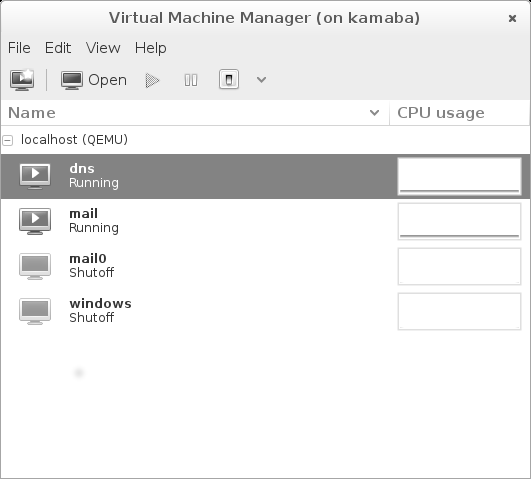
\includegraphics{image201404/virt-manager_mono.png}
\caption{virt-manager$B$N?^(B}
\end{figure*}

\subsubsection{$B2>A[(Bbridge$B$N:n@.(B}
$B<!$K!"2>A[(Bbridge$B$r:n@.$7$^$9!#$3$l$O!"%=%U%H%&%'%"$G(B802.1d Ethernet$B%V%j%C%8$r<BAu$7$F$$$^$9!#(B
$B<j=g$H$7$F$O!"(B
\begin{enumerate}
\item br0$B$r:n@.(B
\item eth0$B$r=i4|2=!"(Bbr0$B$K@\B3(B
\item VM$B$N2>A[(BNIC$B$KBP1~$9$k%$%s%?!<%U%'%$%9$r(Bbr0$B$K@\B3(B
\end{enumerate}

$B6qBNE*$K$O!"(Bvirt-manager$B$rN)$A>e$2!V(BConnection Details$B!W$G!"!V(BNetworkInterfaces$B!W$N!V(BConfigure network interface$B!W$G!V(BBridge$B!W$rA*Br$7!"2>A[(Bbridge$B$K$9$k%G%P%$%9$rA*Br$7$F(BIP$B%"%I%l%9!J(BIPv4$B!K$r$U$j$^$9!#(B

%$B?^7A$NA^F~(B
\begin{figure*}[!b]
\centering
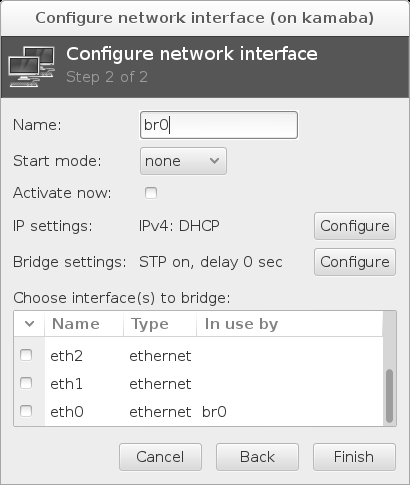
\includegraphics{image201404/bridge2_mono.png}
\caption{bridge$B@_Dj$N>\:Y$N?^(B}
\end{figure*}
\clearpage

$B8e$O!"(BVM$B$r:n@.$9$k$H$-$K%M%C%H%o!<%/$G!V(Bbridge$B!W$rA*Br$9$l$P$$$$$@$1$G$9!#(B
$B%$%a!<%8$H$7$F$O0J2<$N!V?^!W$N$h$&$K$J$j$^$9!#(B

$B$3$3$G(Beth0$B$O!V(Bbridge$B!W$H$7$F30It$K$D$J$,$j$^$9!#$^$?!"%;%-%e%j%F%#$N4X78$+$i(Beth1$B$OJL!V(Bsegment$B!W$K$7!"(Beth0$B$+$iDL?.$r<WCG$7$^$9!#$3$N(Beth1$B$G$O(BSSH$B$J$I$r;HMQ$7!"(Bvirt-manager$B$G3F(BVM$B$r4IM}$7$^$9!#$=$7$F(Beth2$B$O(Beht0$B$HF1$8!V(Bsegment$B!W$K$7$F!"8e=R$N(BSpice$B@lMQ$H$7$^$9!#(B

\begin{figure*}[!h]
\centering
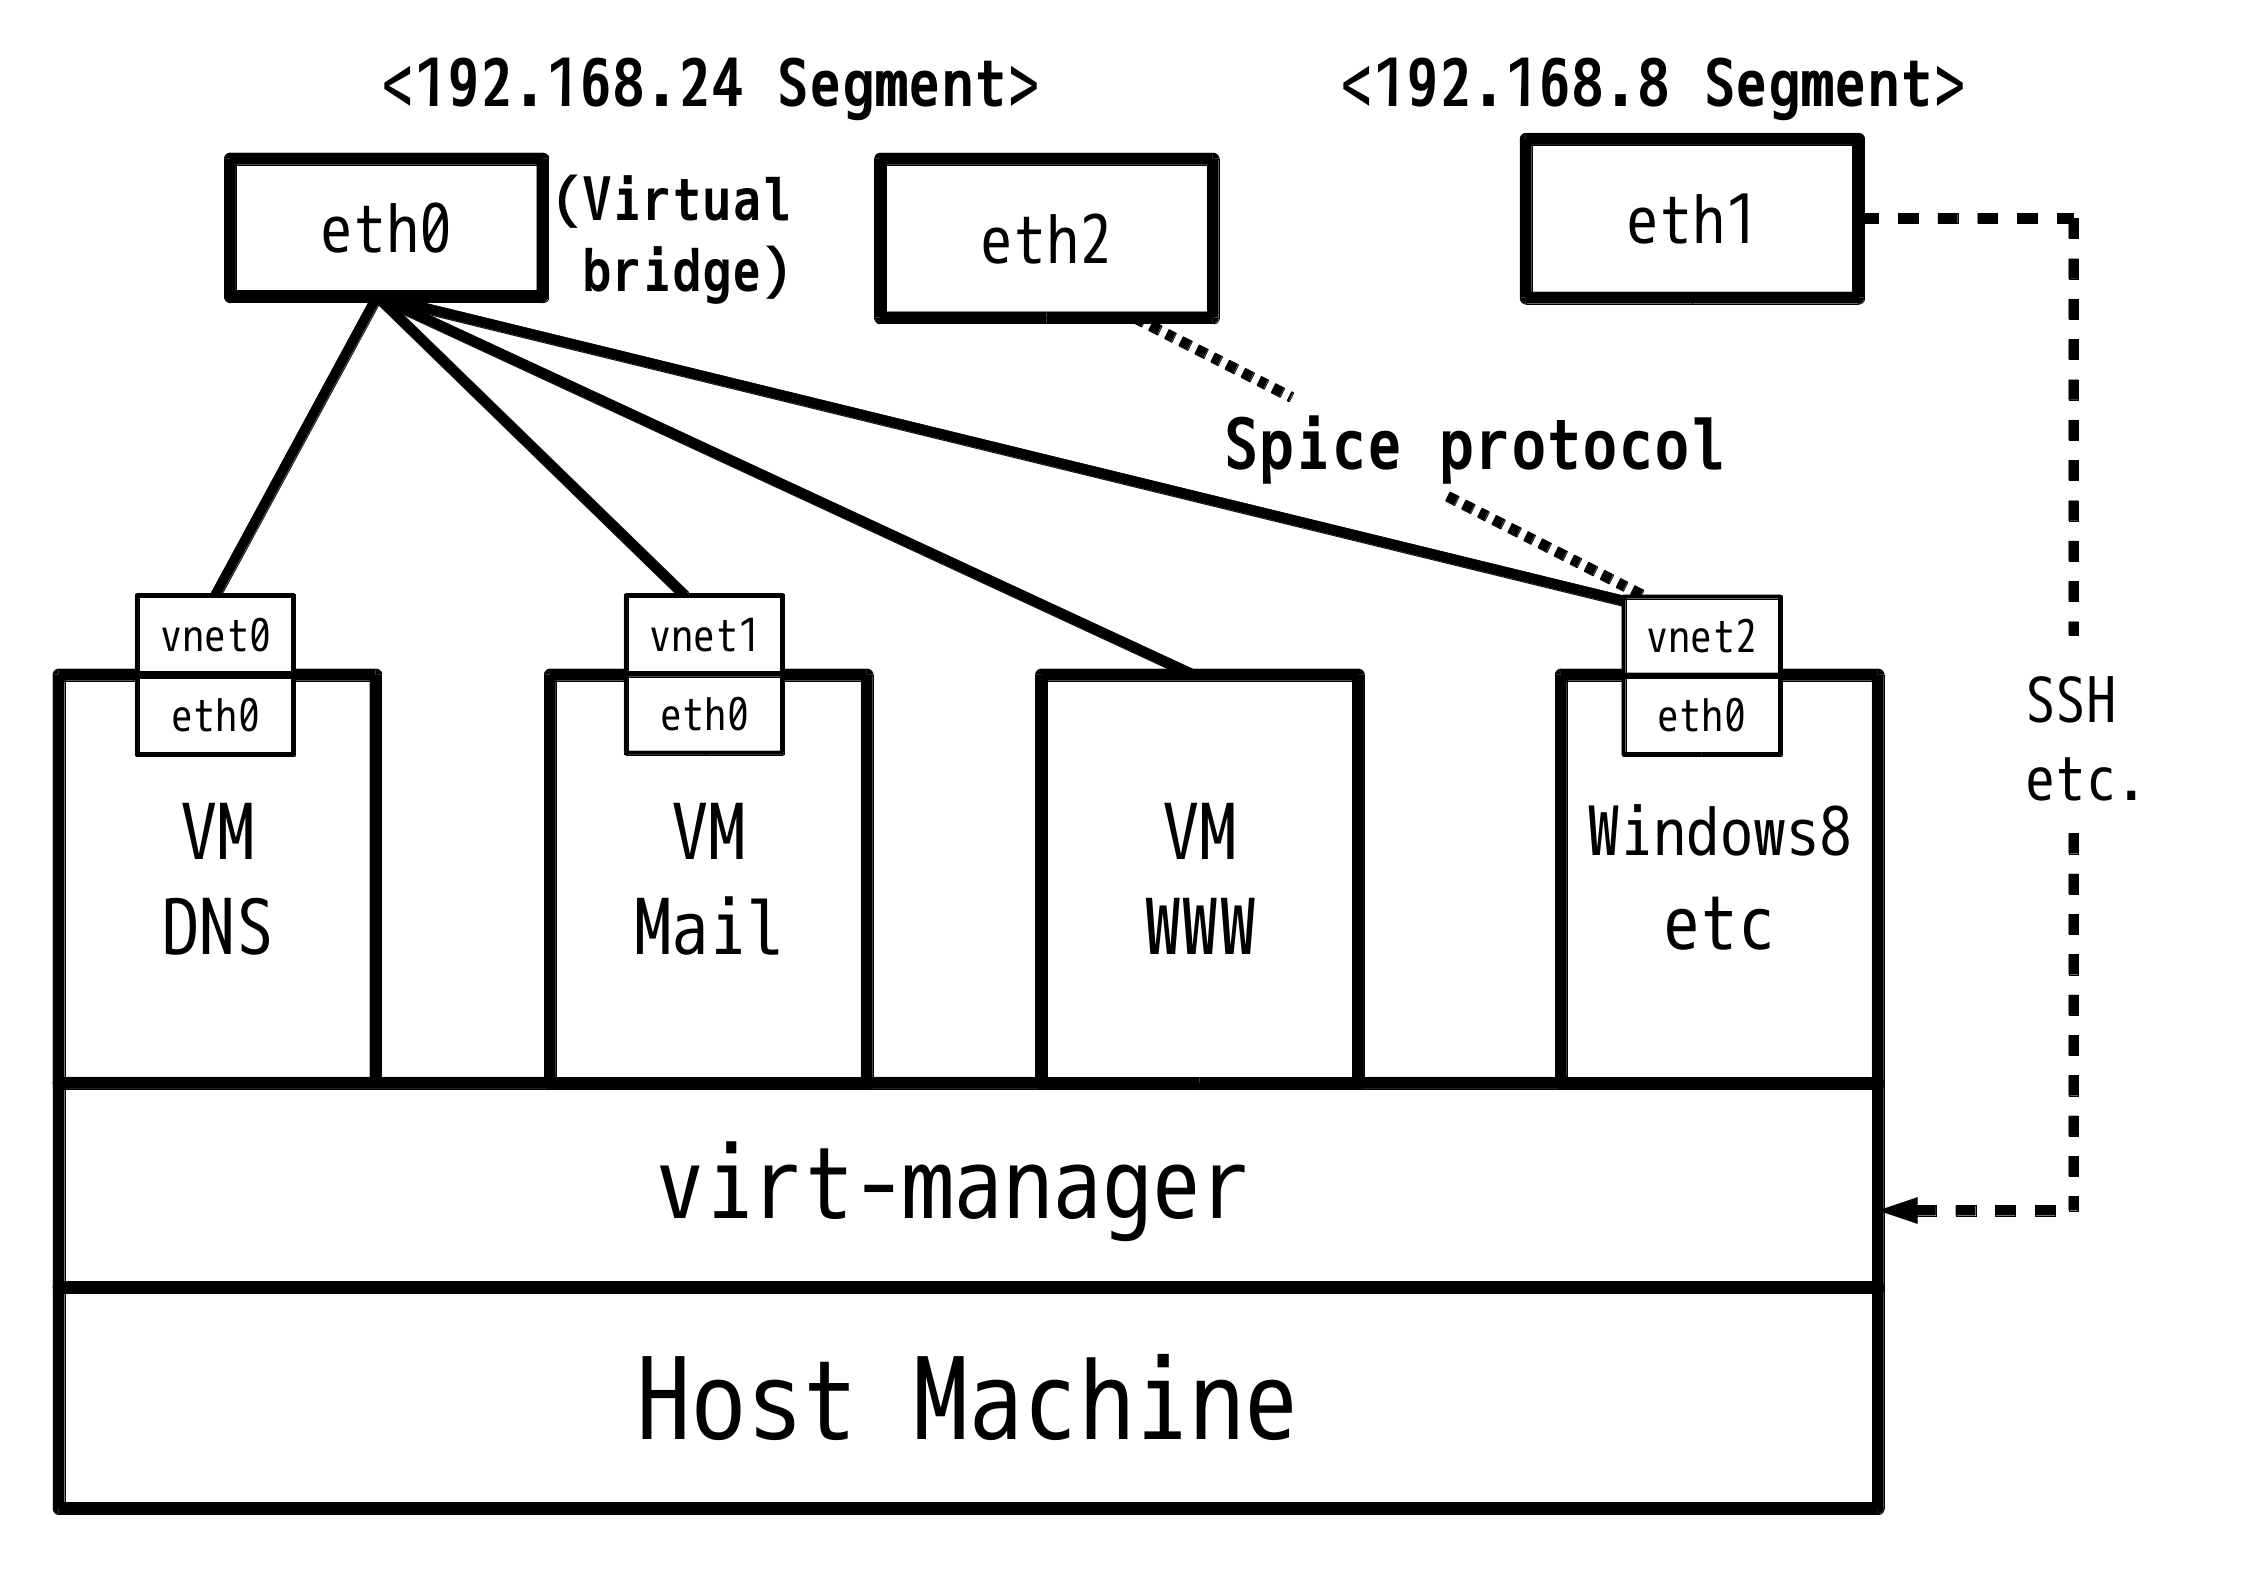
\includegraphics[scale=0.3]{image201404/kvmnetwork3.png}
\caption{$B%M%C%H%o!<%/9=@.$N?^(B}
\end{figure*}

\subsubsection{Virtual Machine$B$N:n@.(B}
$B<!$K!"(Bvirt-manager$B$G(BVM$B$r:n@.$7$^$9!#(Bvirt-manager$B$O(BGUI$B%D!<%k$N%&%#%6!<%I$G!"(BVM$B$N:n@.;~$K$O!"J*M}%^%7%sMQ$N%$%s%9%H!<%k%G%#%9%/!J;THN(BOS$B!K$d(BISO$B%$%a!<%8$r;H$$(BVM$B$r:n@.$7$^$9!#$^$?!"<B%^%7%s$N%j%=!<%9Fb$G$"$l$PMF0W$K(BVM$B$N!V3HD%!W$,$G$-$^$9!#(B
%Hands on$B$K$h$k%$%s%9%H!<%k(B

\clearpage

\subsection{$B3F<o%$%s%?!<%M%C%H4XO"$N%5!<%P$N:n@.(B}
VM$B$N:n@.$,$G$-$?$i!"3F%5!<%P$r:n@.$7$^$9!#$^$:!"(BDNS$B$N:n@.$K$O(Bbind9$B%Q%C%1!<%8$r%$%s%9%H!<%k$7$^$9!#(B
%$B6qBNE*$K(Bwww.kinsen.gr.jp$B$H$$$&%[%9%HL>$KBP1~$9$k(BIP$B%"%I%l%9$r!J:F5"!K8!:w$9$k>l9g!"$^$:!"(Bjp$B%I%a%$%s$N(BIP$B%"%I%l%9$rLd$$9g$o$;$kI,MW$,$"$j$^$9!#$=$N$?$a$K!"%k!<%H%5!<%P$G(Bjp$B%I%a%$%s$N(BIP$B%"%I%l%9$r8!:w$7!"(Bjp$B%5!<%P$K@\B3$7$^$9!#F1MM$K!"(Bjp$B$KB0$9$k(Bgr$B%I%a%$%s$N(BIP$B%"%I%l%9$r8!:w$7!"$5$i$K$O(Bgr$B%I%a%$%s$KB0$9$k(Bkinsen$B$=$7$F(Bwww$B$H=g<!!"3F(BIP$B%"%I%l%9$r8!:w$7!"3F%5!<%P$K@\B3$7$F$$$-$^$9!#$=$7$F:G=*E*$K!"(Bwww.kinsen.gr.jp$B$N(BIP$B%"%I%l%9$,(B203.141.158.41$B$G$"$k;v$,$o$+$j$^$9!#(B
\begin{commandline}
# apt-get install bind9
# apt-get install bind9utils
\end{commandline}
DNS$B$N@_Dj$G$9$,(BNTT$B$N2s@~$N4X78>e!"#18D$N!V%0%m!<%P%k!W(BIP$B%"%I%l%9$7$+;H$($J$+$C$?$N$G!"J#?t$N%m!<%+%k(BIP$B%"%I%l%9$G3F%5!<%P!J%/%i%$%"%s%H!K$K(BIP$B%"%I%l%9$r?6$j$^$9!#$=$3$G!"(Bacl$B!J(BAccess Control List$B!K$G(BIP$B%"%I%l%9$H%M%C%H%o!<%/$r;XDj$7!"(Bacl$B$K%^%C%A$9$k%/%i%$%"%s%H$H!"$=$NB>$N%/%i%$%"%s%H$4$H$KJL!9%>!<%s$rDs6!$7$^$9!#$3$l$rMxMQ$7!"(B1$BBf$N%5!<%P$GFbItMQ!J(Bacl$B$K%^%C%A$9$k!K$H30ItMQ!J(Bacl$B$K%^%C%A$7$J$$!K$N(BDNS$B$r9=C[$7$^$9!#6qBNE*$K$O!"(B
\begin{enumerate}
\item acl$B$G!"%"%I%l%9%^%C%A%j%9%H$r@_Dj!#(B
\item $B%/%i%$%"%s%H!J3F%5!<%P!K$r(BIP$B$K$h$C$F;XDj$7!"%/%i%$%"%s%HKh$N?6$kIq$$$r:n@.!#(B
\item view$B%9%F!<%H%a%s%H$G!"FbIt%/%i%$%"%s%H!"30It%/%i%$%"%s%H$KJL!9$N(Bzone$B%U%!%$%k$r;2>H$5$;$k!#(B
\end{enumerate}
Mailserver$B$K$O!"(BPostfix$B!J(BMTA Mail Transfer Agent$B!K!"(BDovecot$B!J(BMDA Mail Delivery Agent$B!K$r;H$$$^$9!#(B
\begin{commandline}
# apt-get install postfix
# apt-get install dovecot
\end{commandline}
$B$^$:!"(BPostfix$B$K$D$$$F$O!"(Bsasl$B$NG'>Z5!9=$r;H$C$F%f!<%6$NG'>Z!J(BSMPT-AUTH$B!K$r9T$$!"%f!<%6G'>Z$GMQ$$$k%Q%9%o!<%I!JJ?J8!K$r(BTLS$B$G0E9f2=$7$^$9!#$=$7$F!"%a!<%kAw?.$N$?$a$KG'>Z5!G=$N$D$$$?%5%V%_%C%7%g%s%]!<%H$r;HMQ$9$k$?$a$N@_Dj$r$7$^$9!#(B

devecot$B$O(BIMAP$B!J(BInternet Message Access Protocol$B!K%W%m%H%3%k$r;H$$%a!<%k%5!<%P$N%a!<%k$K%"%/%;%9!"A`:n!"%*%U%i%$%s$H%*%s%i%$%s$NAPJ}$GMxMQ$G$-$^$9!#$^$?!"(BMail$B%5!<%P$N9=@.$K$D$$$F$O!"(B
\begin{enumerate}
\item $B<u?.$7$?%a!<%k$r(BMail$B%G%#%l%/%H%j$G07$&$h$&$K@_Dj(B
\item imapcopy$B$r;H$C$F!"5l%a!<%k%5!<%P$h$j%a!<%k%G!<%?$NE>Aw(B
\item $B%&%#%k%9BP:v$K$O!"(Bclamtk$B$r%$%s%9%H!<%k(B
\end{enumerate}

\subsection{$B%5!<%P$N1?MQ!&4IM}(B}
$B%5!<%P!<$N1?MQ!&4IM}$O!"%j%b!<%HA`:n!"%P%C%/%"%C%W!"%P%C%A=hM}$N<B9T!"%H%i%V%k$NM=KI!&H/8+$N$?$a$N2TF/4F;k$J$I$,I,MW$G$9$,!"8D?M$G1?MQ$9$k<+Bp%5!<%P$J$N$G!"(BVM$B$N%/%m!<%s$H(Bimport$B!"(BSPICE$B$r<h$j>e$2$^$9!#(B

\subsubsection{VM$B$N(Bclone$B!"(Bimport}
$B%P%C%/%"%C%W$O!"(BVM$B$G$"$k3F%5!<%P$N%G%#%9%/%$%a!<%8$r%Y!<%9$K!"(Bclone$B$r:n$j$^$9!#$3$N(Bclone$B!J%G%#%9%/%$%a!<%8!K$O%Y!<%9$H$J$C$?(BVM$B$H$^$C$?$/F1$8!V9=@.!W$G$9$,!"(Bvirt-manager$B$r;H$C$F(BMAC$B%"%I%l%9$NJQ99$,$G$-$^$9!#$^$?!"%$%a!<%8$r(BKVM$B$,Av$C$F$$$kJL$N%^%7%s$K(Bimport$B$G$-$^$9!#$^$?!"3F<o%5!<%P$N9=C[$N:]$O!V%Y!<%9$N(BVM$B!W$r:n@.$7!"%/%m!<%s$r:n$C$F!X%+%?%^%$%:!Y$9$k$J$I$N;H$$J}$,$G$-$^$9!#(B

\subsubsection{SPICE}
$B%j%b!<%HA`:n$K$O(BSPICE$B$r;H$$$^$9!#(BSPICE$B!J(BSimple Protocol for Independent Computing Environment$B!K$O!"2>A[2=4D6->e$K9=C[$7$?%G%9%/%H%C%W4D6-$K%j%b!<%H$+$i@\B3$9$k$H$$$&2>A[%G%9%/%H%C%W4D6-!J(BVDI$B!K$G$9!#FCD'$O!"%*!<%W%s%=!<%9$N2hLLE>Aw%W%m%H%3%k$G!"9b2h<A$J%S%G%*E>Aw$H9b2;<A$JAPJ}8~2;@<E>Aw$,$G$-$k$3$H$G$9!#(B

$B<!$K!"(Bspice$B%/%i%$%"%s%H$r%$%s%9%H!<%k$7!"%?!<%_%J%k$+$i@\B3$7$^$9!#(B
\begin{commandline}
# apt-get install spice-client
\end{commandline}
$BB3$$$F!"(Bqemu-kvm$B$N(BVM$B$K@\B3$7$^$9!#(B
\begin{commandline}
$ spicec -h noren.kinsen.gr.jp -p 590X -w *********
\end{commandline}
$B!V(B-h$B!W$O%[%9%HL>!"!V(B-p$B!W$O%]!<%HHV9f!"!V(B-w$B!W$O%m%0%$%s$9$k$?$a$N%Q%9%o!<%I$G$9!#(B

\subsection{$B$^$H$a(B}
$B$^$H$a$H$7$F!"<+J,$N<+Bp%5!<%P$O$3$N4V!"(B2$BG/$[$I!V(BXen$B!W$G1?MQ$7$F$$$^$7$?!#(BXen$B$O(Bqemu-kvm$B$HF1$8%O%$%Q!<%P%$%6$J$N$G$9$,!"2>A[2=$N%b%G%k$,=`2>A[2=$J$N$G!"%5!<%P$KB?$/$N%j%=!<%9$OI,MW$"$j$^$;$s!J%a!<%k%5!<%P!"(BDNS$B$H$b$I$b(B384MB$B$G1?MQ$7$^$7$?!K!#$?$@!"%j%=!<%9$,==J,$KMQ0U$G$-$k$N$G$"$l$P!"(BOS$B$r(Bdefault$B$G;H$($kE@$d!"(Bvirt-manager$B$J$I$N%D!<%k!"!V9bB.!W!V9b5!G=!W$N(BSPICE$B$,;HMQ$G$-$k$J$I$NMxE@$,(Bqemu-kvm$B$K$O$"$j$^$9!#(B

$B:#8e$NM=Dj$H$7$F$O!"(BWWW$B%5!<%P$G$O!V(BHTML5$B!W$r;H$C$?%5%$%H$N9=C[$d!"(BIPv6$B$X$NBP1~!J$?$@$7!"%Q!<%=%J%k%l%Y%k$G(BGlobal Routing Prefix$B$,(B /48-/64bit$BFb$G$"$k$3$H$,A0Ds!K!"$5$i$J$k!X0[<o!Y$N(BOS$B$N(BVM$B2=$r$7$?$$$H;W$C$F$$$^$9!#(B

%201404 tokyo
%-------------------------------------------------------------------------------
\dancersection{Golang$B$G=q$+$l$?%D!<%k$r(BDebian$B%Q%C%1!<%8$K$9$k(B}{$BA0ED(B $B9LJ?(B}
%-------------------------------------------------------------------------------
\index{Golang}
\index{dh-golang}

\subsection{$B$O$8$a$K(B}

$B$"$k$3$H$r$d$k$N$K(BSerf\footnote{\url{http://www.serfdom.io/}}$B$H$$$&%D!<%k$,NI$$$N$G$O!"$HF1N=$K=u8@$r$b$i$C$?$N$G!"(BSerf$B$G$d$j$?$$$3$H$,$G$-$J$$$+8!>Z$r$9$k$3$H$K$7$^$7$?!#$G$9$,!"$=$b$=$b(BDebian$B%Q%C%1!<%8$K$OL5$$$N$G$^$:$=$3$+$i$G$7$g!"$H$$$&$3$H$G<j85$G(BDebian$B%Q%C%1!<%8$K$7$^$7$?!#(B\footnote{Serf$B<+BN$N$*OC$rJ9$-$?$$$H;W$C$?J}$O;DG0!#(BUpstream\footnote{\url{https://github.com/hashicorp/serf/}}$B$N%I%-%e%a%s%H$dF|K\8l$N(BSerf$B$r;H$C$?%*!<%1%9%H%l!<%7%g%s$N;qNA$r8+$?$@$1$G!"(BSerf$B<+BN$N8!>Z$O$^$@9T$C$F$$$J$$$N$G!"(BSerf$B$=$N$b$N$K$D$$$F$O2?$b8l$l$^$;$s!#(B}

Serf$B$r(BDebian$B%Q%C%1!<%8$K$9$k$K$"$?$j!"9T$C$?$3$H$d!"(BGolang$B$N%D!<%k$r(BDebian$B%Q%C%1!<%8$K$9$k>e$GI,MW$JCN<1!"<j=g$r$^$H$a$^$7$?!#:#2s$NJY6/2q$G$O!"(BDebian$B%Q%C%1!<%8$r=i$a$F:n@.$9$k?M$N3d9g$,Hf3SE*B?$+$C$?$N$G!"FbMFE*$K>/$7>iD9$K$J$C$F$$$^$9!#(B

\subsection{Debian$B$G$N(BGolang$B$N4D6-9=C[(B}

\subsubsection{$BA0Ds>r7o(B}

$B;HMQ$9$k%G%#%9%H%j%S%e!<%7%g%s$O!"(BDebian GNU/Linux Sid$B$rA0Ds$H$7$^$9!#<j85$K(BSid$B$N4D6-$,$J$$>l9g$O!"2>A[%^%7%s$J$I$GMQ0U$7$F$/$@$5$$!#(B

\subsubsection{Debian$B%Q%C%1!<%8$N%$%s%9%H!<%k(B}

Debian$B$G$O!"(B ``golang'' $B$H$$$&%a%?%Q%C%1!<%8$,MQ0U$5$l$F$$$^$9!#$3$l$r%$%s%9%H!<%k$9$k$H<!$N%Q%C%1!<%8$,%$%s%9%H!<%k$5$l$^$9!#(B\footnote{Linux Kernel$B$N(B amd64$B%"!<%-%F%/%A%c$N>l9g(B}

\begin{itemize}
\item golang-doc \\
  \url{http://golang.org}$B$N%I%-%e%a%s%H!#(B\texttt{godoc --http=:6060} $B$r<B9T$7!"(B\url{http://localhost:6060/}$B$G1\Mw2D(B
\item golang-go \\
  Golang$B$N%"%;%s%V%i!"%3%s%Q%$%i!<!"%j%s%+!<$J$I$N%D!<%k%A%'%$%s(B
\item golang-go-linux-amd64 \\
  Linux$B%7%9%F%`!"(Bamd64$B%"!<%-%F%/%A%c8~$1$NI8=`%i%$%V%i%j!#(Bsystem: darwin,freebsd,linux,netbsd,windows$B!"(Barch: amd64,386,arm
\item golang-go.tools \\
  Golang$BMQ$NJd=u%D!<%k!#A0=R$N(Bgodoc$B%3%^%s%I$b4^$^$l$k(B
\item golang-src \\
  golang$B%Q%C%1!<%8$N%=!<%9%3!<%I!#(Bgodoc$B%3%^%s%I$J$I$G;H$o$l$k(B
\item libjs-jquery \\
  jQuery$B!#(Bgolang-go.tools$B$K0MB8!#(Bgodoc$B%3%^%s%I$G<B9T$9$k(Bgolang-doc$B$N%I%-%e%a%s%HMQ(B
\item javascript-common \\
  JavaScript$B%i%$%V%i%j%Q%C%1!<%8$N%5%]!<%H%Q%C%1!<%8!#(Blibjs-jquery$B$K0MB8(B
\end{itemize}

\subsection{Golang$B$N%3%s%Q%$%kJ}K!(B}

$BI8=`%i%$%V%i%j$N$_$G=q$+$l$?%3!<%I$r%3%s%Q%$%k$9$k>l9g$K$O!"(B\texttt{go build}$B%3%^%s%I$N$_$G$G$-$^$9!#(B
$BNc$($P!"$*$J$8$_$K(BHello world$B$N%3!<%I(B(hello.go)$B$rMQ0U$7$^$9!#(B

\begin{commandline}
package main

import "fmt"

func main() {
  fmt.Println("Hello world.")
}
\end{commandline}

$B%3%s%Q%$%k$7$^$9!#(B

\begin{commandline}
$ go build hello.go

\end{commandline}

$B%P%$%J%j$N<B9T$O(B\texttt{./hello}$B$G$9!#(B

\begin{commandline}
$ ./hello
Hello world.
\end{commandline}

\texttt{file}$B%3%^%s%I$G8+$k$H!"@EE*%j%s%/$5$l$F$$$k$3$H$,J,$+$j$^$9!#(B

\begin{commandline}
$ file hello
hello: ELF 64-bit LSB executable, x86-64, version 1 (SYSV), statically linked, not stripped
\end{commandline}

$B$J$*!"(B\texttt{go run}$B%3%^%s%I$r;H$&$H!"%3%s%Q%$%k$7$J$/$F$b<B9T2DG=$G$9!#(B
\begin{commandline}
$ rm hello
$ go run hello.go
Hello world.
$ ls hello
ls: cannot access hello: No such file or directory
\end{commandline}

\subsubsection{$BI8=`%i%$%V%i%j0J30$K0MB8$9$k(BGolang$B%Q%C%1!<%8$N%3%s%Q%$%k(B}

$B$^$:!"0MB8$9$k%Q%C%1!<%8$NG[CV>l=j$r4D6-JQ?t(B\texttt{GOPATH}$B$G;XDj$9$kI,MW$,$"$j$^$9!#(B

$B%7%9%F%`%0%m!<%P%k$N@_Dj$O!"(BDebian$B$G$O!"(B\texttt{/usr/share/gocode}$B$K$J$j$^$9!#4{$K(BDebian$B%Q%C%1!<%8$K$J$C$F$$$k(BGolang$B$N%i%$%V%i%j$O!"$3$N%G%#%l%/%H%j$N2<$K$"$k!"(Bsrc$B%G%#%l%/%H%j0J2<$K%$%s%9%H!<%k$5$l$^$9!#(B

$B%7%9%F%`%0%m!<%P%k$G@_Dj$5$l$F$$$k%Q%C%1!<%8$r;H$&>l9g$K$O!"(B

\begin{commandline}
$ export GOPATH=/usr/share/gocode
\end{commandline}

GOPATH$B$O@dBP%Q%9$G;XDj$9$kI,MW$,$"$j$^$9!#(B
$B%3%s%Q%$%k$9$k%3!<%I$HF1$8%+%l%s%H%G%#%l%/%H%j$KB8:_$9$k$J$i!"(B
\begin{commandline}
$ export GOPATH=$(pwd)
\end{commandline}

$B$H<B9T$7$?>e$G!"<B:]$N%Q%C%1!<%8$NG[CV$O!"(B
\texttt{\$(pwd)/src/example.org/mkouhei/hoge/}$B$N$h$&$J%G%#%l%/%H%j9=@.$K$J$C$F$$$kI,MW$,$"$j$^$9!#(B
$B@h$[$I$N(Bhello.go$B$K$3$N%Q%C%1!<%8$r(Bimport$B$9$k>l9g!"(B

\begin{commandline}
import (
    "fmt"
    "example.org/mkouhei/hoge"
)
\end{commandline}

$B$N$h$&$K$J$j$^$9!#(B

$B$J$*!"I8=`%i%$%V%i%j$O!"(BDebian$B$G$O!"(B\texttt{/usr/lib/go}$B0J2<$K%$%s%9%H!<%k$5$l$F$$$^$9!#I8=`%i%$%V%i%j%i%$%V%i%j$O!"(BGOPATH$B$G;XDj$9$kI,MW$O$J$/!"(BGOROOT$B$H$$$&4D6-JQ?t$G!"(B\texttt{/usr/lib/go}$B$,@_Dj$5$l$F$$$^$9!#(B

GOPATH$B$,@_Dj$5$l$F$$$l$P!"%Q%C%1!<%8$N%@%&%s%m!<%I$H%$%s%9%H!<%k$O(B\texttt{go get}$B%3%^%s%I$G9T$($^$9!#(B\footnote{\url{http://golang.org/cmd/go/\#hdr-Download_and_install_packages_and_dependencies}}

\texttt{GOPATH}$B$G;XDj$7$?%G%#%l%/%H%j0J2<$K!"2<5-$N$h$&$J7A$G<+F0E*$K%$%s%9%H!<%k$5$l$^$9!#(B

\begin{commandline}
$ go get example.org/mkouhei/hoge
$ tree
.
|-- pkg
|   `-- linux_amd64
|       `-- example.org
|           `-- mkouhei
|               `-- hoge.a
`-- src
    `-- example.org
        `-- mkouhei
            `-- hoge
                |-- LICENSE
                |-- README.rst
                `-- hoge.go
\end{commandline}

\texttt{GOPATH}$B$r@_Dj$7!"(Bimport$B$G$-$l$P!"(B\texttt{go build}$B$O0MB84X78$r2r7h$7$F%3%s%Q%$%k$G$-$^$9!#(B
$B%P%$%J%j$N$_$r(BDebian$B%Q%C%1!<%8$K$9$k:]$K!"(B\texttt{GOPATH}$B$,=EMW$G$9!#(B

\subsection{Golang$B$G=q$+$l$?%=%U%H%&%'%"$N(BDebian$B%Q%C%1!<%8:n@.J}K!(B}

Golang$B$G=q$+$l$?%=%U%H%&%'%"$N(BDebian$B%Q%C%1!<%8:n@.J}K!$K$D$$$F@bL@$7$^$9!#(B
$BBg$-$/<!$N(B2$B%Q%?!<%s$,$"$j$^$9!#(B

\begin{itemize}
\item $B%P%$%J%j$N$_(B
\item $B%i%$%V%i%j$N$_!J$b$7$/$O%i%$%V%i%j$H%P%$%J%j!K(B
\end{itemize}

$BA0<T$G$O%3%s%Q%$%k$,I,MW$G$9!#(BGolang$B$N>l9g!"0MB8$9$k%i%$%V%i%j$rA4$F@EE*$K%j%s%/$9$k$?$a!"%P%$%J%j$N<B9T$=$N$b$N$K$O0MB84X78$O$"$j$^$;$s!#$G$9$N$G!"%G!<%b%s2=$9$k%1!<%9$G$J$1$l$P!"(BDepends$B$K5-=R$9$k%Q%C%1!<%8$,4pK\I,MW$"$j$^$;$s!#(B\footnote{$B%G!<%b%s2=$7$F(BOS$B5/F0;~$K<+F05/F0$9$k>l9g!"%m%0$N%m!<%F!<%7%g%s$G(Blogrotate$B$K0MB8$7$?$j!"@lMQ%f!<%6$r:n$C$F<B9T$5$;$k$N$K(Badduser$B$,I,MW$G$9!#(B}

$B8e<T$G$O!"4pK\E*$K$O%3%s%Q%$%k$=$N$b$N$OI,MW$"$j$^$;$s!#$7$+$7!"A0=R$N(B/usr/share/gocode$B2<$K%=!<%9%3!<%I$r%$%s%9%H!<%k$9$kI,MW$,$"$k$N$G!"(Bdh-golang$B%Q%C%1!<%8$r(BBuild-Depends$B5-=R$7!"(Bdebian/rules$B$G!"(B\texttt{dh}$B%3%^%s%I$K(B\texttt{--with=golang}$B%*%W%7%g%sEO$7$F$d$kI,MW$,$"$j$^$9!#(B

$B$^$?!"%P%$%J%j!"%i%$%V%i%j$KLd$o$:!"0MB8$9$k(BGolang$B$N%Q%C%1!<%8$rA4$F(BBuild-Depends$B$K5-=R$9$kI,MW$,$"$j$^$9!#(B\footnote{$B$3$l$O(BGolang$B$K8B$C$?OC$G$O$"$j$^$;$s$M!#(B}$B$^$?!"(BGolang$B$G$O(B\texttt{go test}$B$G%F%9%H$r<B9T$7$?$j!"(B\texttt{go build}$B$d(BMakefile$B$G%3%s%Q%$%k$9$k>l9g!"0MB8$9$k(BGolang$B%Q%C%1!<%8$r(B\texttt{go get}$B$G(BGOPATH$B$G;XDj$7$?%G%#%l%/%H%j$K%@%&%s%m!<%I$*$h$S%$%s%9%H!<%k$5$l$k$N$G$9$,!"(BDebian$B%Q%C%1!<%8$N%S%k%I$G$O!"(B\texttt{go get}$B$r;H$o$J$$$h$&$K$7$J$/$F$O$$$1$^$;$s!#(B

\subsubsection{Debian$B%Q%C%1!<%8:n@.MQ$N4D6-@_Dj(B}

$B$^$:(Bdh-golang$B%Q%C%1!<%8$r%$%s%9%H!<%k$7$^$9!#(BDebian$B%Q%C%1!<%8<+BN$r:n$C$?$3$H$,L5$/!"0l$+$i4D6-$r@0$($k!"$H$$$&?M$O!"<!$N%3%^%s%I$r<B9T$7$^$9!#(B

\begin{commandline}
$ sudo apt-get devscripts debhelper fakeroot dh-golang cowbuilder piuparts git git-buildpackage
\end{commandline}

git$B$*$h$S(Bgit-buildpackage\footnote{git-buildpackage$B$O%=!<%9%Q%C%1!<%8<+BN$r(BGit$B$G4IM}$9$k$?$a$N%D!<%k$G$9!#(B}$B$OI,?\$G$O$"$j$^$;$s!#$7$+$7!"(BGolang$B$G=q$+$l$?$N%D!<%k$NB?$/$O(BGit$B%j%]%8%H%j$G4IM}$5$l$F$$$^$9!#$^$?!"@N$J$,$i$N%P!<%8%g%K%s%0$,$5$l$J$$%1!<%9$,$[$H$s$I$G$9!#$=$N$?$a!"(Btarball$B<+BN$NDs6!$b$5$l$J$$$b$N$,B?$$$N$G!"(BGit$B$,DL>oI,MW$K$J$j$^$9!#(B

$B$^$?(BGolang$B$N(BDebian$B%Q%C%1!<%8$N%a%s%F%J%s%9%A!<%`(B(the pkg-go team\footnote{\url{http://pkg-go.alioth.debian.org/}})$B$G$O!"(Bgit-buildpackage$B$G%=!<%9%Q%C%1!<%8$r4IM}$9$k$3$H$K$J$C$F$$$^$9!#(B\footnote{\url{http://pkg-go.alioth.debian.org/packaging.html\#_packaging_in_git}}

$B$J$*!"A0=R$N(B\texttt{go get}$B%3%^%s%I$G$O!"%j%]%8%H%j$+$iF~<j$7$F!"$=$N$^$^(B\texttt{GOPATH}$B$G@_Dj$7$?%G%#%l%/%H%j$N(Bsrc$B%G%#%l%/%H%j0J2<$KE83+$5$l$F$7$^$&$N$G!"%P!<%8%g%s$d%3%_%C%H$,J,$+$i$J$$$N$G;H$o$J$$J}$,$h$$$G$7$g$&!#$J$*!"(BBuild-Depends$B$G$N0MB84X78$N2r7h$N:]$K$b!"(BDebian$B%Q%C%1!<%8%s%0%]%j%7!<>e!"(B\texttt{go get}$B%3%^%s%I$O;H$($^$;$s!#(B

.bashrc$B$K2<5-$N$h$&$JJQ?t$r@_Dj$7$^$9!#(B
\begin{commandline}
export DEBFULLNAME='Kouhei Maeda'
export DEBEMAIL=mkouhei@palmtb.net
\end{commandline}

pbuilder, cowbuilder$B$N(Bchroot$B%$%a!<%8$r:n@.$7$^$9!#(B\footnote{pbuilder$B$O(Bcowbuilder$B$r%$%s%9%H!<%k$9$k$H<+F0E*$K%$%s%9%H!<%k$5$l$^$9!#(B}

\begin{commandline}
$ sudo pbuilder --create
$ cowbuilder --create
\end{commandline}
pbuilder$B$NJ}$O!"(B/var/cache/pbuilder/base.tgz$B$,!"(Bcowbuilder$B$NJ}$O(B/var/cache/pbuilder/base.cow$B$,:n@.$5$l$^$9!#(B

\subsubsection{$B%i%$%V%i%j$N%Q%C%1!<%8:n@.(B}

$B$^$:(BUpstream$B$N(Btarball$B$b$7$/$O(BSCM$B$N%j%]%8%H%j$rF~<j$7$^$9!#A0=R$NDL$j!"(BGit$B$G4IM}$5$l$F$$$k%1!<%9$rA[Dj$7$^$9!#(B

Serf$B$N%S%k%I$N0MB84X78$G(B($B4V@\E*$K(B)$BI,MW$K$J$C$?(B\url{https://github.com/huin/gobinarytest}$B$rNc$K$7$^$9!#(B\texttt{git clone}$B$7$?$i!"%V%i%s%A$H%?%0!"%m%0$r3NG'$7$^$9!#(B

\begin{commandline}
$ git clone https://github.com/huin/gobinarytest.git
$ cd gobinarytest
$ git branch -a
* master
  remotes/origin/HEAD -> origin/master
  remotes/origin/master
$ git tag -l
$ git log | head -5
commit de322f729af68c9e5ecde2bff780d105f0fbe745
Author: Huin <greatred@gmail.com>
Date:   Tue Feb 11 22:50:34 2014 +0000

    Add LICENSE
\end{commandline}

Golang$B$G=q$+$l$?%D!<%k$O!"$3$NDL$j!"EAE}E*$J%P!<%8%g%s%K%s%0$,$5$l$J$$$3$H$,B?$$$G$9!#(B\texttt{go get}$B%3%^%s%I$r;H$($P!"0MB84X78$N$"$k%Q%C%1!<%8$N:G?7$N%3%_%C%H$rF~<j$G$-$k$3$H$,1F6A$7$F$$$k$N$G$O$J$$$+$H!!;W$$$^$9!#(B

pkg-go team$B$N%]%j%7!<$H$7$F!"$3$&$$$&%1!<%9$K$O!"(B0.0~gitYYYYMMDD$B$N$h$&$J%P!<%8%g%s$r$D$1$k;v$K$J$C$F$$$^$9!#(B\footnote{\url{http://pkg-go.alioth.debian.org/packaging.html\#_version_numbers}}

$B$^$?!"(BDebian$B%Q%C%1!<%8$r:n@.$9$k$H$-$NL?L>5,B'$b$"$j$^$9!#(BGolang$B$N>l9g!"(BPerl$B$N(BCPAN$B$d!"(BPython$B$N(BPyPI$B$N$h$&$J8x<0$K0l854IM}$7$F$$$k%Q%C%1!<%8%j%]%8%H%j$,B8:_$7$J$$$N$G!"(BGit$B$N%j%]%8%H%jL>$@$1$r;H$&$HL>A0$,6%9g$9$k2DG=@-$,$"$j$^$9!#(B\footnote{Serf$B$r%Q%C%1!<%82=$9$k:]$K$b<B:]$K$"$j$^$7$?!#(B}

$B$=$3$G!"%i%$%V%i%j%Q%C%1!<%8$r:n@.$9$k>l9g!"(Bgithub.com/huin/gobinarytest$B$N>l9g$K$O!"(Bgolang-huin-gobinarytest-dev $B$H$$$&%Q%C%1!<%8L>$K$7$^$9!#(B\footnote{\url{http://pkg-go.alioth.debian.org/packaging.html\#_naming_conventions_2}}

$B$G$O!"$^$:(B\texttt{git archive}$B%3%^%s%I$r;H$C$F(Btarball$B$r:n$j$^$9!#(B

\begin{commandline}
$ git archive --prefix=golang-huin-gobinarytest/ HEAD | gzip > ../golang-huin-gobinarytest-0.0~git20140211.tar.gz
\end{commandline}

$B<!$K(BDebian$B%Q%C%1!<%8MQ$N(BGit$B%j%]%8%H%j$r:n@.$7!"(Btarball$B$r%$%s%]!<%H$7$^$9!#(B

\begin{commandline}
$ cd -
$ mkdir golang-huin-gobinarytest
$ cd golang-huin-gobinarytest
$ git init
$ git import-orig ../golang-huin-gobinarytest-0.0~git20140211.tar.gz
What will be the source package name? [golang-huin-gobinarytest]
What is the upstream version? [0.0~git20140211]
gbp:info: Importing '../golang-huin-gobinarytest-0.0~git20140211.tar.gz' to branch 'master'...
gbp:info: Source package is golang-huin-binarytest
gbp:info: Upstream version is 0.0~git20140211
gbp:info: Successfully imported version 0.0~git20140211 of ../golang-huin-gobinarytest-0.0~git20140211.tar.gz
\end{commandline}

$B<!$K(B\texttt{dh\_make}$B%3%^%s%I$G(Bdebian$B%G%#%l%/%H%j$r@8@.$7$^$9!#$3$N%Q%C%1!<%8<+BN$O(B2$B>r9`(B BSD$B%i%$%;%s%9$J$N$G!"(B\texttt{--copyright}$B%*%W%7%g%s$G;XDj$7$^$9!#:n@.8e!"ITMW$J%F%s%W%l!<%H$O:o=|$7$^$9!#%i%$%V%i%j%Q%C%1!<%8$G$9$,!"(B

\begin{commandline}
$ dh_make -l --copyright bsd -p golang-huin-gobinarytest_0.0~git20140211 -f ../golang-huin-gobinarytest-0.0~git20140211.tar.gz
$ cd debian
$ ls
README.Debian  golang-huin-gobinarytest-dev.dirs     init.d.ex        preinst.ex
README.source  golang-huin-gobinarytest-dev.install  manpage.1.ex     prerm.ex
changelog      golang-huin-gobinarytest.cron.d.ex    manpage.sgml.ex  rules
compat         golang-huin-gobinarytest.default.ex   manpage.xml.ex   shlibs.local.ex
control        golang-huin-gobinarytest.doc-base.EX  menu.ex          source
copyright      golang-huin-gobinarytest1.dirs        postinst.ex      watch.ex
docs           golang-huin-gobinarytest1.install     postrm.ex
$ rm README* golang-huin-gobinarytest* init.d.ex manpage.* menu.ex post* pre* shlibs.local.ex watch.ex
$ ls
changelog  compat  control  copyright  docs  rules  source
\end{commandline}

$B2<5-$N$h$&$KJQ99$7$^$9!#(B

\subsubsubsection{debian/control}

Golang$B$N%Q%C%1!<%8$K$O!"(BBuild-Depends$B$K(Bgolang-go$B$H!"(B
$B$^$?(BGolang$B$N%i%$%V%i%j%Q%C%1!<%8$O(BDepends$B$K$b(Bgolang-go$B$H!"$^$?(BBuild-Depends$B$K(Bdh-golang$B$r5-=R$7$^$9!#(B
$B%i%$%V%i%j$N(Bgolang-huin-gobinary-test-dev$B%Q%C%1!<%8$O!"%=!<%9%3!<%I$J$N$G!"(BArchitecture$B$O(Ball$B$K$7$^$9!#(B

\begin{commandline}
Source: golang-huin-gobinarytest
Section: devel
Priority: optional
Maintainer: Kouhei Maeda <mkouhei@palmtb.net>
Build-Depends: debhelper (>= 9.0.0), dh-golang, golang-go
Standards-Version: 3.9.5
Homepage: https://github.com/huin/gobinarytest

Package: golang-huin-gobinarytest-dev
Architecture: all
Depends: golang-go
Description: Helper code for unit testing binary encoding code
 The gobinarytest package is used in testing serialization and
 deserialization. It is particularly useful when some sub-sequences of bytes
 can acceptably be written in any order (e.g if they are generated from
 representations that do not provide order guarantees like maps).
\end{commandline}

\subsubsubsection{debian/rules}
Golang$BMQ$N%]%$%s%H$H$7$F$O!"(B\texttt{dh}$B%3%^%s%I$K!"(B\texttt{--buildsystem=golang}$B%*%W%7%g%s$H!"(B\texttt{--with=golang}$B%*%W%7%g%s$r;XDj$9$k$3$H$G$9!#(B

$B%i%$%V%i%jMQ$K$O!"@h$[$I$N(B\texttt{GOPATH}$B$N2<$GE83+$5$l$k%Q%C%1!<%8$N%M!<%`%9%Z!<%9$r4D6-JQ?t(B\texttt{DH\_GOPKG}$B$G;XDj$7$^$9!#$3$N%M!<%`%9%Z!<%9$O!"DL>o8x3+$7$F$$$k%j%]%8%H%j$N(BURL$B$,%Y!<%9$K$J$j$^$9$,!">l9g$K$h$C$F$O<B:]$K8x3+$7$F$$$k(BURL$B$H$OJL$N%j%@%$%l%/%H85$N(BURL$B$r;XDj$9$k$3$H$3$H$b$"$j$^$9!#(Bupstream$B$N%I%-%e%a%s%H$d%=!<%9%3!<%I$r3NG'$7$F$_$F$/$@$5$$!#(B
$B$^$?!"(B\texttt{override\_dh\_auto\_install}$B$rDj5A$7!"(B\texttt{dh\_auto\_install -O-buildsystem=golang}$B$G>e=q$-$7$^$9!#$3$l$K$h$j!"$3$N%Q%C%1!<%8$r%S%k%I8e!"(Bgolang-huin-gobinarytest-dev$B%Q%C%1!<%8$r%$%s%9%H!<%k$9$k$H!"A0=R$N(B/usr/share/gocode$B$N2<$K%=!<%9%3!<%I$,%$%s%9%H!<%k$5$l$^$9!#(B

\begin{commandline}
#!/usr/bin/make -f
# -*- makefile -*-

# Uncomment this to turn on verbose mode.
#export DH_VERBOSE=1

export DH_GOPKG := github.com/huin/gobinarytest

%:
        dh $@ --buildsystem=golang --with=golang

override_dh_auto_install:
        dh_auto_install -O-buildsystem=golang
\end{commandline}

$B$3$NNc$G$O!"B>$N(BGolang$B%Q%C%1!<%8$K0MB8$7$F$$$J$$$N$G;H$C$F$$$^$;$s$,!"B>$N%Q%C%1!<%8$K0MB8$9$k>l9g$O!"(B

\begin{commandline}
export GOPATH := $(CURDIR)_build:/usr/share/gocode
\end{commandline}

$B$N$h$&$J@_Dj$,I,MW$K$J$j$^$9!#(B

\subsubsubsection{debian/copyright}
\begin{commandline}
ormat: http://www.debian.org/doc/packaging-manuals/copyright-format/1.0/
Upstream-Name: gobinarytest
Source: https://github.com/huin/gobinarytest

Files: *
Copyright: 2013, John Beisley <greatred@gmail.com>
License: BSD-2-Clause

Files: debian/*
Copyright: 2014 Kouhei Maeda <mkouhei@palmtb.net>
License: BSD-2-Clause

License: BSD-2-Clause
 Redistribution and use in source and binary forms, with or without
 modification, are permitted provided that the following conditions
 are met:
 1. Redistributions of source code must retain the above copyright
    notice, this list of conditions and the following disclaimer.
 2. Redistributions in binary form must reproduce the above copyright
    notice, this list of conditions and the following disclaimer in the
    documentation and/or other materials provided with the distribution.
 .
 THIS SOFTWARE IS PROVIDED BY THE COPYRIGHT HOLDERS AND CONTRIBUTORS
 ``AS IS'' AND ANY EXPRESS OR IMPLIED WARRANTIES, INCLUDING, BUT NOT 
 LIMITED TO, THE IMPLIED WARRANTIES OF MERCHANTABILITY AND FITNESS FOR
 A PARTICULAR PURPOSE ARE DISCLAIMED.  IN NO EVENT SHALL THE HOLDERS OR
 CONTRIBUTORS BE LIABLE FOR ANY DIRECT, INDIRECT, INCIDENTAL, SPECIAL, 
 EXEMPLARY, OR CONSEQUENTIAL DAMAGES (INCLUDING, BUT NOT LIMITED TO, 
 PROCUREMENT OF SUBSTITUTE GOODS OR SERVICES; LOSS OF USE, DATA, OR 
 PROFITS; OR BUSINESS INTERRUPTION) HOWEVER CAUSED AND ON ANY THEORY OF 
 LIABILITY, WHETHER IN CONTRACT, STRICT LIABILITY, OR TORT (INCLUDING 
 NEGLIGENCE OR OTHERWISE) ARISING IN ANY WAY OUT OF THE USE OF THIS 
 SOFTWARE, EVEN IF ADVISED OF THE POSSIBILITY OF SUCH DAMAGE.
\end{commandline}

\subsubsubsection{debian/changelog}

\texttt{dch -r}$B%3%^%s%I$r<B9T$7$^$9!#(B

\begin{commandline}
golang-huin-gobinarytest (0.0~git20140211-1) unstable; urgency=low

  * Initial release (Closes: #nnnn)

 -- Kouhei Maeda <mkouhei@palmtb.net>  Wed, 12 Feb 2014 14:47:33 +0900
\end{commandline}

$B$"$H$O(Bgolang-huin-gobuildtest$B%G%#%l%/%H%j$N2<$G!"(B\texttt{git buildpackage}$B%3%^%s%I$r<B9T$9$k$H!"M=$a(B\texttt{cowbuilder --create}$B%3%^%s%I$G:n@.$7$F$*$$$?(B/var/cache/pbuilder/base.cow$B$N(Bchroot$B%$%a!<%8$r;H$C$F!"%Q%C%1!<%8$,%S%k%I$5$l$^$9!#(B

\subsubsection{$B%P%$%J%j$N%Q%C%1!<%8:n@.(B}

$BBg$^$+$JN.$l$O%i%$%V%i%j$N>l9g$HF1$8$G$9!#0[$J$k$N$O!"(B

\begin{itemize}
\item $B%Q%C%1!<%8$NL?L>5,B'(B \\
  golang- $B$H$$$&(Bprefix$B$r$D$1$kI,MW$O$J$$!#(B\footnote{Serf$B$N>l9g$O!"%=!<%9%Q%C%1!<%8$,(Bserf$B$H$J$C$F$$$k!"(BHTTP client library(libserf1)$B$,$"$k$N$G!"%P%C%F%#%s%0$9$k$N$G%=!<%9%Q%C%1!<%8L>$O(Bgolang-serf$B$H$9$k$+!"(BDocker$B$N$h$&$K(Bserf.io$B$H$9$k$N$,NI$5$=$&!#(B}
\item debian/control$B$N(BBuild-Depends$B$K(Bdh-golang$B$,ITMW(B\footnote{$B%i%$%V%i%j$r4^$a$k>l9g$OI,MW$G$9!#(B}
\item debian/control$B$N%P%$%J%jMQ$N%Q%C%1!<%8$N(BArchitecure$B$,(Ball$B$G$O$J$/!"(Bany
\item debian/rules$B$G!"(B\texttt{dh}$B%3%^%s%I$K(B\texttt{--with=golang}$B%*%W%7%g%s$OITMW(B(dh-golang$BMQ$N%*%W%7%g%s$N$?$a(B)
\end{itemize}

$B$H$$$&$"$?$j$G$9!#(B

Serf\footnote{\url{https://github.com/hashicorp/serf}}$B$r%Q%C%1!<%8$K$9$k>l9g$N@_DjNc$O2<5-$G$9!#(B

\subsubsection{debian/control}

Build-Depends$B$NCf$G!"%i%$%V%i%j$N>l9g$H0c$&$N$O(Btxt2man$B$H(Bdh-systemd$B$G$9!#(B
$B<B9T2DG=$J%P%$%J%j%U%!%$%k$O!"(BDebian$B%Q%C%1!<%8$N%]%j%7!<>e!"(Bman$B%^%K%e%"%k$rMQ0U$9$kI,MW$,$"$j$^$9!#(B
$B$7$+$7!"(Bserf$B$O%3%^%s%I%i%$%s%X%k%W$O=<<B$7$F$$$k$b$N$N!"(Bman$B%^%K%e%"%k$O$"$j$^$;$s!#(B
$B$J$N$G!"(Btxt2man$B$r;H$C$F<+F0@8@.$7$^$7$?!#(B

dh-systemd$B$O!"(Bsystemd$BMQ$NJd=u%D!<%k$G$9!#(B

\begin{commandline}
Source: golang-serf
Section: web
Priority: optional
Maintainer: Kouhei Maeda <mkouhei@palmtb.net>
Build-Depends: debhelper (>= 9.0.0),
        golang-go (>= 2:1.2),
        golang-hashicorp-memberlist-dev,
        golang-mitchellh-cli-dev,
        golang-hashicorp-logutils-dev,
        golang-mitchellh-mapstructure-dev,
        golang-ugorji-go-dev,
        golang-armon-mdns-dev (>= 0.0~git20140225~8be7e3a),
        golang-ryanuber-columnize-dev,
        dh-systemd,
        txt2man
Standards-Version: 3.9.5
Homepage: http://www.serfdom.io/

Package: serf
Architecture: any
Depends: ${shlibs:Depends}, ${misc:Depends}, adduser
Description: Service orchestration and management tool
 Serf is a service discovery and orchestration tool that is decentralized,
 highly available, and fault tolerant. Serf runs on every major platform:
 Linux, Mac OS X, and Windows. It is extremely lightweight: it uses 5 to 10 MB
 of resident memory and primarily communicates using infrequent UDP messages.
\end{commandline}

\subsubsubsection{debian/rules}

Serf$B$K$O!"(BMakefile$B$,$D$$$F$$$k$N$G$9$,!"%S%k%I$KA0=R$N(B\texttt{go get}$B%3%^%s%I$r;H$C$F!"0MB8$9$k%Q%C%1!<%8$r%+%l%s%H%G%#%l%/%H%j$K%@%&%s%m!<%I!u%$%s%9%H!<%k$7$F$$$^$9!#(BDebian$B%Q%C%1!<%8$N:n@.$N%]%j%7!<>e!"%S%k%ICf$K%j%b!<%H%[%9%H>e$N%j%=!<%9$r<hF@$7$F$O$$$1$J$$$N$G!"(Bupstream$B$N(BMakefile$B$r$=$N$^$^MxMQ$G$-$^$;$s!#$=$N$?$a!"%+%l%s%H%G%#%l%/%H%j$H!"%7%9%F%`%0%m!<%P%k$K@_Dj$7$?(BGOPATH$B$+$i!"0MB8%Q%C%1!<%85Z$S!"(BSerf$B<+?H$G%$%s%]!<%H$7$F$$$k%3!<%I$r;H$&$h$&$K$7$F$$$k$N$,!"(B\texttt{override\_dh\_auto\_build}$B$N=hM}$G$9!#(B

$B$^$?!"A0=R$N(Bman$B%^%K%e%"%k$N@8@.$O!"(B\texttt{override\_dh\_installman}$B$N=hM}$G9T$C$F$$$^$9!#(B

\begin{commandline}
#!/usr/bin/make -f
# -*- makefile -*-

# Uncomment this to turn on verbose mode.
#export DH_VERBOSE=1

export DH_GOPKG := github.com/hashicorp/serf
GOPATH := ${CURDIR}/_build:/usr/share/gocode
BLDPATH := obj-$(shell dpkg-architecture -qDEB_BUILD_GNU_TYPE)
export LANG := C

export GOPATH

%:
        dh $@ --buildsystem=golang --with=systemd

override_dh_auto_build:
        mkdir -p ${CURDIR}/_build/src/${DH_GOPKG}
        cp -a ${CURDIR}/*.go ${CURDIR}/serf ${CURDIR}/client \
                ${CURDIR}/command ${CURDIR}/testutil ${CURDIR}/_build/src/${DH_GOPKG}/
        go build -v -o ${CURDIR}/_build/serf

override_dh_auto_test:
        cd $(CURDIR)/_build && \
        go list ./... | xargs -n1 go test && \
        $(CURDIR)/scripts/setup_test_subnet.sh && \
        go list ./... | INTEG_TESTS=yes xargs -n1 go test

override_dh_auto_install:
        install -d ${CURDIR}/debian/serf/usr/bin
        test -f ${CURDIR}/_build/serf && \
        install -m 0755 ${CURDIR}/_build/serf ${CURDIR}/debian/serf/usr/bin/

override_dh_installman:
        test -f ${CURDIR}/_build/serf && \
        ${CURDIR}/_build/serf -h 2>&1 | txt2man -t SERF -s 1 -v 'Serf Manual' > ${CURDIR}/debian/serf.1
        set -e && ${CURDIR}/_build/serf -h 2>&1 | grep -v version | grep -E '^\s+\w+' | while read line; do \
                subcmd=`echo $$line | awk '{print $$1}'`;\
                desc=`echo $$line | awk '{ $$1=""; print }'`;\
                ${CURDIR}/_build/serf $$subcmd -h 2>&1 | txt2man -t SERF-`echo $$subcmd | tr "[:lower:]" "[:upper:]"`
 -s 1 -v 'Serf Manual' > $(CURDIR)/debian/serf-$$subcmd.1; \
                sed -i "/Serf Manual/a .SH NAME\nserf-$$subcmd \- $$desc" $(CURDIR)/debian/serf-$$subcmd.1 ;\
        done
        sed -i '/Serf Manual/a .SH NAME\nserf \- Service orchestration and management tool' $(CURDIR)/debian/serf.1
        sed -i '/[Uu]sage:/i .SH SYNOPSIS' $(CURDIR)/debian/serf*.1
        sed -i '/Available commands are:/i .SH OPTIONS' $(CURDIR)/debian/serf*.1
        sed -i 's/^Options:/.SH OPTIONS/g' $(CURDIR)/debian/serf*.1
        sed -i 's/-/\\-/g' $(CURDIR)/debian/serf*.1
        dh_installman ${CURDIR}/debian/serf*.1

override_dh_auto_clean:
        dh_clean
        rm -rf ${CURDIR}/_build
        rm -rf ${CURDIR}/${BLDPATH}
        rm -f ${CURDIR}/debian/serf*.1

DEB_UPSTREAM_VERSION=$(shell dpkg-parsechangelog | sed -rne 's,^Version: ([^+]+).*,\1,p')
get-orig-source:
        uscan --noconf --force-download --rename --download-current-version --destdir=.
        rm -rf serf-$(DEB_UPSTREAM_VERSION)
        tar xf golang-serf_$(DEB_UPSTREAM_VERSION).orig.tar.gz
        rm -f golang-serf_$(DEB_UPSTREAM_VERSION).orig.tar.gz
        rm -rf serf-$(DEB_UPSTREAM_VERSION)/website
        GZIP=--best tar cz --owner root --group root --mode a+rX \
                -f ../golang-serf-$(DEB_UPSTREAM_VERSION)+dfsg.orig.tar.gz \
                serf-$(DEB_UPSTREAM_VERSION)
        rm -rf serf-$(DEB_UPSTREAM_VERSION)
\end{commandline}


\subsection{Serf$B$N0MB8$9$k%Q%C%1!<%8(B}

$B:G8e$K!"(BSerf$B$,(BBuild-Depends$B$GI,MW$H$J$j!"$+$D!"$^$@(BDebian$B%Q%C%1!<%8$K$J$C$F$$$J$$%Q%C%1!<%8$r?^<($7$F$*$-$^$9!#;M3Q$N%N!<%I$,%Q%C%1!<%8$K$J$C$F$$$J$$$b$N$G$9!#(B

\includegraphics[width=15cm]{image201404/serf-dependency.eps}

\begin{thebibliography}{0}
  \bibitem{command-go}
    {\footnotesize{
        The Go Programming Language, ``Command go'',
        \url{http://golang.org/cmd/go/}}}
  \bibitem{debian-go-packaging}
    {\footnotesize{
        Alioth, ``Debian Go Packaging'',
        \url{http://pkg-go.alioth.debian.org/packaging.html}}}
\end{thebibliography}

%201401 kansai LT$B$N$?$a$J$7(B
%201402 kansai LT$B$N$?$a$J$7(B
%201402 tokyo OSC Tokyo$B$N$?$a$J$7(B
%201403 kansai LT$B$N$?$aL5$7(B
%201405 kansai $B$b$/$b$/2q$N$_$N$?$aL5$7(B

%-------------------------------------------------------------------------------
\dancersection{Debian Trivia Quiz}{$BLnEg(B $B5.1Q(B}
%-------------------------------------------------------------------------------

$B$H$3$m$G!"$_$J$5$s(B Debian $B4XO"$NOCBj$K$*$$$D$$$F$$$^$9$+!)(BDebian$B4XO"$NOC(B
$BBj$O%a!<%j%s%0%j%9%H$r$h$s$G$$$k$HDI@W$G$-$^$9!#$?$@$h$s$G$$$k$@$1$G$O$O(B
$B$j$"$$$,$J$$$N$G!"M}2rEY$N%F%9%H$r$7$^$9!#FC$K0l?M$@$1$G$O0UL#$,$o$+$i$J(B
$B$$$H$3$m$b$"$k$+$bCN$l$^$;$s!#$_$s$J$G0l=o$KFI$s$G$_$^$7$g$&!#(B

$B:#2s$N=PBjHO0O$O(B\url{debian-devel-announce@lists.debian.org} $B$d(B \url{debian-devel@lists.debian.org}$B$KEj9F$5$l$?(B
$BFbMF$H(BDebian Project News$B$+$i$G$9!#(B

\begin{multicols}{2}
%; whizzy-master ../debianmeetingresume201311.tex
% $B0J>e$N@_Dj$r$7$F$$$k$?$a!"$3$N%U%!%$%k$G(B M-x whizzytex $B$9$k$H!"(Bwhizzytex$B$,MxMQ$G$-$^$9!#(B
%

\santaku
{2013/12/15$B$K=P$?(BDebian wheezy$B$N%"%C%W%G!<%H$N%P!<%8%g%s$O!)(B}
{7.3}
{7.2}
{7.1}
{A}
{debian wheezy$B$r$*;H$$$N3'MM$OAaB.%"%C%W%G!<%H$7$^$7$g$&!*(B}

\santaku
{Debian$B$b;22C$7$F$$$k(BFOSS$B9W8%<T$K=w@-$rA}$d$=$&1?F0$N;v$r$J$s$H$$$&!)(B}
{Encourage Women in Linux}
{Outreach Program For Women}
{IT$B@o;N(B}
{B}
{Outreach Program For Women($BN,$7$F(BOPW)$B$O!"(B\\
\url{http://gnome.org/opw/}
$B$K>pJs$,$"$j$^$9!#(B}

\santaku
{$B@hF|(BDebian$B$N(BTechnical Committee$B$K%a%s%P$,A}$($^$7$?!#$H$3$m$G!"(B
 $B8=:_$N(BTechnical Comittee$B$N(Bchair man$B$OC/$G$7$g$&(B?}
{Takahide Nojima}
{Lucas Nussbaum}
{Bdale Garbee}
{C}
{$B85(BHP$B$N(BLinux$BItLg$N(BCTO$B$rL3$a$?$H$$$&7PNr$N;}$A<g$G$9!#(Bdebconf$B$H$+$K(B
$B;22C(B/$B%S%G%*;kD0$H$+$9$k$H$o$+$k$N$G$9$,!">oO"$5$s$N$h$&$G$9!#(B}


%; whizzy-master ../debianmeetingresume201311.tex
% 以上の設定をしているため、このファイルで M-x whizzytex すると、whizzytexが利用できます。
%

\santaku
{PHPのメンテナチームを3つに分割する事が提案されました。分割されたグループの名前で間違っているのはどれ?}
{Debian PHP PECL Maintainers}
{Debian PHP PEAR Maintainers}
{Debian PHP DOCUMENT Maintainers}
{C}
{正しくは''Debian PHP Maintainers''です。以前、Debian PHP Maintainersは、PHP本体のパッケージも、PEARモジュールのパッケージも両方メンテナンスしていました。}

\santaku
{Debianについて、Debian Developer以外の人でも貢献したを讃えましょうということで、作られたサイトは?}
{advocates.debian.org}
{contributors.debian.org}
{superstar.debian.org}
{B}
{Debianに貢献したDebian Developer以外の人のアカウントが\url{http://contributors.debian.org/}にリストアップされるようになりました。なお、貢献についての集計の元は、\url{https://contributors.debian.org/sources/}に掲載されている情報を元に集計しているとの事です。}

\santaku
{2013/12後半頃にs390xアーキテクチャのデフォルトCコンパイラとしてのgccのバージョンが変更されました。どのバージョンになったのでしょう?}
{4.8}
{4.7}
{4.6}
{A}
{2013/12/23現在、powerpc/ia64/sparcアーキテクチャのデフォルトCコンパイラはまだgcc 4.6のようです。Debianの次期バージョンのJessieではgcc 4.6はサポート対象外なので早いところgcc 4.6から脱却する必要があります。}

\santaku
{2014/1に有名なデータベースがパッケージとして追加されました。何というデータベースでしょうか?}
{Maria DB}
{Percona DB}
{GDB}
{A}
{Maria DBは、LAMPシステムで有名なMysql DBの別の実装です。ついにMaria DBキター!今後のMysql依存のDebianのパッケージの動向が気になるこの頃です。}



%; whizzy-master ../debianmeetingresume201311.tex
% $B0J>e$N@_Dj$r$7$F$$$k$?$a!"$3$N%U%!%$%k$G(B M-x whizzytex $B$9$k$H!"(Bwhizzytex$B$,MxMQ$G$-$^$9!#(B
%

\santaku
{$B@hF|!"<!4|(BDebian$B$N%P!<%8%g%s$G$"$k(BJessie$B$K$F!"$H$"$k%"!<%-%F%/%A%c$N%5%]!<%H$,BG$A@Z$i$l$^$7$?!#$=$l$O!"$I$N%"!<%-%F%/%A%c!)(B}
{hurd-i386}
{s390x}
{ia64}
{C}
{$BD9$$4V$*Hh$l!*!d(Bia64$B!#(BAMD$B$N@oN,$KIi$1$?!"@$4V$KIi$1$?!#$H$3$m$G!"(Bhurd-i386$B%"!<%-%F%/%A%c$H(Bsparc$B%"!<%-%F%/%A%c$b!"(BRelease Team$B$K$h$l$P$o$j$H33$C$W$A$J>u67$N$h$&$G$9!#;29M!'(B\url{https://lists.debian.org/debian-devel-announce/2014/01/msg00008.html}}

\santaku
{$B:#7n(B2$B7n$"$?$^$K%j%j!<%9$5$l$?(Bstable$BHG$N(BDebian$B$N%P!<%8%g%s$O$$$/$D$G$7$g$&!)(B}
{7.3}
{7.4}
{7.5}
{B}
{wheezy$B;H$$$N?M$OAaB.%"%C%W%G!<%H$@!*:#2s$b%;%-%e%j%F%#$K4X$9$k(BBugfix$B$,<g$G$9!#(B}

\santaku
{Debian$B$N;q;:(B(Asset$B$N;v$G$9(B)$B$rG$$;$k$3$H$N$G$-$k!V?.Mj$KB-$kAH?%(B(Trusted Organization)$B!W$NDj5A$,@hF|%l%S%e!<$5$l$F$$$^$7$?!#?.Mj$KB-$kAH?%$N>r7o$KEv$F$O$^$i$J$$AH?%$O$I$l(B}
{$B8x<0(BDebian$B3+H/<T$,5o$J$$AH?%(B}
{$BAGAa$$1~Ez(B/$BBP1~$,$G$-$kAH?%(B}
{Debian$B<R2q7{>O$HBPN)$7$J$$AH?%(B}
{A}
{$B:G?7HG$O!"(B\url{https://wiki.debian.org/Teams/DPL/TrustedOrganizationCriteria}
$B$K7G:\$5$l$F$$$^$9!#$A$J$_$K!"?.Mj$KB-$kAH?%$,2?$r$9$k$N$+$NDj5A$K$D$$$F$O!"(BDebian$B%W%m%8%'%/%H7{>O$N(B9.4$B>O$K$"$j$^$9!#:#$^$GL@3N$J4p=`$,$J$+$C$?$N$+!)$H$$$&$N$,$A$g$C$H6C$-!#(B}

\santaku
{1/23$B$K(BPC$B%2!<%`$r%M%C%H$GGd$k%5!<%S%9(B(Steam)$B1?1D$GM-L>$J(BValve$B<R$,!"$$$/$D$+$N(BLinux$BBP1~$N%2!<%`$rL5NA$GDs6!$7$^$9$H7h$a$^$7$?!#$I$s$J?M$,BP>]$G$7$g$&$+!)(B}
{$BA4(BDebian$B%f!<%6(B}
{$BA4(BDebian$B8x<03+H/<T(B}
{$BA4(BIT$B4k6H$N(BDebian$B%5!<%P!<@o;N(B}
{B}
{$B$3$l$b%3%_%e%K%F%#$X$N4k6H$N4sIU$NJ}K!$H$7$FLLGr$$$H;W$$$^$7$?!#(B}


\santaku
{Debian$B$N8xJs%A!<%`$,!"%=!<%7%c%k%a%G%#%"$N8x<0%"%+%&%s%H$G$NH/8@$9$kFbMF$NJg=8$r$7$F$$$^$9!#:G=i$KEj9F$5$l$k$N$O$I$N%"%+%&%s%H$G$7$g$&$+!)(B}
{twitter$B$N(Bdebian}
{google$B!\$N(Bdebian}
{identi.ca$B$N(Bdebian}
{C}
{debian$B$N%=!<%7%c%k%a%G%#%"$N8x<0%"%+%&%s%H$+$i(BDebian$B$N3hF0$r%"%T$j$?$$?M$O1~Jg$7$F$_$k$HNI$$$H$*$b$$$^$9!#(B\url{https://wiki.debian.org/Teams/Publicity/Identica}}




%; whizzy-master ../debianmeetingresume201311.tex
% 以上の設定をしているため、このファイルで M-x whizzytex すると、whizzytexが利用できます。
%

\santaku
{2014年GSoCのメンター募集が行われています。2014年のGSoCにて採択されていないものはどれ}
{hurd-i386の開発}
{clangでDebianのパッケージをコンパイルできるようにする}
{Android上でDebian環境を作れる件の改良を行う}
{A}
{他にもいろいろなProjectがDebian Projectから採択されています。Elektra\url{http://www.libelektra.org}で設定ファイルのアップグレードを改良するとか、libstdc++からlibc++を使うようにDebianを変更する件や、パッケージ管理にMuonを使う件など。参考:\url{https://wiki.debian.org/SummerOfCode2014/Projects}}

\santaku
{2014/2/14にバグレポートのIDが\#740000を向かえました。\#730000からどのぐらいの期間がたったでしょう?}
{1ヶ月と3日}
{3ヶ月と4日}
{10ヶ月と10日}
{B}
{毎年、Christian Perrierさんにより、バグレポートのIDについて、将来いつ何万番台を迎えるかについて当てるコンテストが行われています。}

\santaku
{Debianのコミュニティにより提供されているWebサービスについて調査が行われています。この調査の名前は?}
{Debian Services Servey}
{Outreach Program For Women}
{Debian Services Census}
{C}
{2014/2/13に呼びかけが行われました。現在のサービスの名前とURLのリストは、\url{https://wiki.debian.org/Services}にまとめられています。}

\santaku
{毎年恒例のDPL選挙が始まりました。2014年のDPL立候補者は誰?}
{Takahide Nojima}
{Lucas Nussbaum}
{Stefano Zacchiroli}
{B}
{lucusは2013年DPLですが、2年連続立候補となります。他の2名の方は、Gergely Nagyさん、Neil McGovernさんとなります。
 選挙期間は2014/3/31〜4/13となります。各候補者の声明は、\url{http://www.debian.org/vote/2014/platforms/}に掲載予定です。}

%; whizzy-master ../debianmeetingresume201311.tex
% $B0J>e$N@_Dj$r$7$F$$$k$?$a!"$3$N%U%!%$%k$G(B M-x whizzytex $B$9$k$H!"(Bwhizzytex$B$,MxMQ$G$-$^$9!#(B
%

\santaku
{2015$BG/$N(BDebconf15$B$N3+:E9q$O$I$3$K$J$C$?$G$7$g$&!)(B}
{$B%\%9%K%"!&%X%k%D%'%4%S%J(B}
{$B%&%/%i%$%J(B}
{$B%I%$%D(B}
{C}
{$B:#EY$O%I%$%D$@$=$&$G$9!#$A$J$_$K:#G/$N(BDebconf14$B$O(B8/23-31$B$G(BUSA$B$N(BPortland,Oregon
$B$G3+:EM=Dj$G$9!#(B}

\santaku
{DPL$BA*5s$,9T$o$l$^$7$?!#:#G/$N(BDPL$B$OC/$K$J$C$?$G$7$g$&$+!)(B}
{Lucas Nussbaum}
{Neil McGovern}
{Rapha\"{e}l Hertzog}
{A}
{$B:#G/$N(BDPL$B$N8uJd<T$O#2L>$G!"(BLucas Nussbaum$B$5$s!"(BNeil McGovern$B$5$s$N#2L>(B
$B$G$7$?!##2L>$H$b<+A&$H$N$3$H$G$9!#A*5s$N7k2L!"(B
Lucas Nussbaum(lucus)$B$5$s$N05>!$@$C$?$h$&$G$9!#$A$J$_$K!"(B
Rapha\"{e}l Hertzog$B$5$s$O!"(BThe Debian 
Administrator\'s handbook$B$N:n<T!"B>$K$b0N6H$,$?$/$5$s!#(B}

\santaku
{clang3.4$B$K$h$k(BDebian$B%Q%C%1!<%8$N:F9=C[$,9T$o$l$^$7$?!#7k2L2?(B\%$B$N%Q%C%1!<%8$,@.8y$7$?$G$7$g$&$+!)(B}
{90\%}
{50\%}
{10\%}
{A}
{\url{http://clang.debian.net/}$B$,(Bclang$B$K$h$k(BDebian$B%Q%C%1!<%8:F9=C[$N%]!<%?%k%5%$%H$G$9!#KhG/!"(Bclang$B$N%P!<%8%g%s$r>e$2$F!"A4(BDebian$B%Q%C%1!<%8$r:F9=C[$7$?7k2L$,:\$j$^$9!#:#G/$N7k2L$H$7$F$O:F9=C[BP>]$N%Q%C%1!<%8$N?t$,5nG/$HBgI}$KA}$($F$$$k$K$b$+$+$o$i$:!"9=C[<:GT$K=*$o$C$?%Q%1!<%8?t$,5nG/$HJQ$o$i$J$+$C$?$H$$$&Hs>o$KNI$$7k2L$H$J$C$F$$$^$9!#(B}

\santaku
{beagle board$B%7%j!<%:$H$$$&Hs>o$K?M5$$N$"$k(BARM$B$N<B83%\!<%I$K%P%s%I%k$5$l$k(BOS$B$N>-Mh$N8+DL$7$K$D$$$F!"(Bbeagle board$B$NAON)<T$,$I$N(BOS$B$K$9$kM=Dj$HH/8@$7$?$+!)(B}
{Gentoo}
{Debian$B$C$7$g!*(BDebian}
{Andoroid OS}
{B}
{\url{http://opensource.com/life/14/3/interview-jason-kridner-beagleboard}
$B$K$F!">-Mh(BDebian$B$K$9$k$H$$$&H/8@$,$"$j$^$9!#$H$3$m$G!"(Bbeagle board$B%7%j!<%:$OL$$@$K(BOMAP$B$r(B
$B;H$$B3$1$k$N$+$,6=L#DE!9$G$O$"$j$^$9!#(B}

\santaku
{$B7cO@$NKv!"(B3$B7nCf=\:"$K(BDebian$B$N(Bca-certificates$B%Q%C%1!<%8$+$i>C$($?(Broot$B>ZL@=q$,$"$j$^$9!#$=$l$O$J$s$G$7$g$&!)(B}
{RapidSSL$B$N(Broot$B>ZL@=q(B}
{CAcert$B$N(Broot$B>ZL@=q(B}
{Verisign$B$N(Broot$B>ZL@=q(B}
{B}
{$B5DO@$N%5%^%j$O!"(BLWN$B$N5-;v(B\url{https://lwn.net/Articles/590879/}$B$,H=$j$d$9$$$G$9!#$^$?!"(BCAcert$B$C$F2?!)$H$$$&J}$O!"Bh(B71$B2sEl5~%(%j%"(BDebian$BJY6/2q(B(2010$BG/(B12$B7n3+:E(B)\url{http://tokyodebian.alioth.debian.org/2010-12.html}$B$K7G:\$5$l$F$$$kJY6/2q;qNA$,$*4+$a$G$9!#(B}

\santaku
{Jessie$B$K$F%G%9%/%H%C%W4D6-$rA*Br$7$?:]$KF3F~$5$l$k!"%G%U%)%k%H%3%_%e%K%1!<%7%g%s%D!<%k$N8uJd$K$D$$$F5DO@$,$5$l$F$$$j$^$9!#0J2<$N$I$l$G$7$g$&!)(B}
{Empathy}
{licq}
{jitsi}
{C}
{Debian$B$G$O!"%G%U%)%k%H$N%3%_%e%K%1!<%7%g%s%D!<%k$H$7$F!"$[$\40A4$K(BRTC/VoIP$B$r%5%]!<%H$9$k$3$H$,K>$^$7$$$H$5$l$?$?$a!"$3$A$i$K8~$$$F$$$k%D!<%k$H$7$F:#$^$G$N(BEmpathy$B$h$j$b(Bjitsi$B$,8~$$$F$$$k$N$G$O!)$H$$$&$3$H$+$i5DO@$,3+;O$5$l$^$7$?!#(B}

\santaku
{$B@hF|(BDebian$B$K(BOTR$B%A!<%`$H$$$&(BOTR$B%=%U%H$r%Q%C%1!<%82=$9$k%0%k!<%W$,7k@.$5$l$^$7$?!#$H$3$m$G(BOTR$B$C$F$J$s$NN,!)(B}
{Owa-Tte-Ru}
{OpticalTRacking}
{Off-the-Record}
{C}
{Off-the-Record$B$H$O!"0E9f2=5;=Q$r;H$C$F%$%s%U%iDs6!<T$K$9$i%a%C%;!<%8$N$d$j$H$j$NFbMF$r8+$;$J$$!J5-O?$5$;$J$$!K%a%C%;!<%8%5!<%S%9$rL\;X$7$?$b$N$G$9(B\url{https://www.otr.im/}$B!#(B}

\santaku
{$B@hF|!"(BDebian squeeze$B$N%5%]!<%H4|4V$,?-$S$k@k8@$,(BDSA$B$K$h$j%"%J%&%s%9$5$l$^$7$?!#7k6I$$$D$K$J$C$?!)(B}
{2015/2}
{2016/2}
{2016/5}
{B}
{Long Term Support(LTS)$B$@$=$&$G$9(B\url{https://lists.debian.org/debian-security-announce/2014/msg00082.html}$B!#M=Dj$G$O!"(B2014/5/31$B:"$K%5%]!<%H=*N;$9$k$O$:$G$7$?$N$G!"#2G/<e$N1dD9$H$J$j$^$9!#$?$@%5%]!<%H1dD9$5$l$k$N$O!"(BDebian squeeze$B$NA4It$N%Q%C%1!<%8$G$O$J$$$N$G!"%5%]!<%H$5$l$J$$%Q%C%1!<%8$r==J,$K$*;H$$$N3'MM$O!"(BDebian wheezy$B$X%"%C%W%0%l!<%I$9$k$3$H$r$*4+$a$7$F$*$-$^$9!#(B}



%; whizzy-master ../debianmeetingresume201311.tex
% 以上の設定をしているため、このファイルで M-x whizzytex すると、whizzytexが利用できます。
%

\santaku
{2014/4/26に、とあるアーキテクチャがtestingから外されました。次のうちのどれでしょう?}
{i386}
{armel}
{sparc}
{C}
{リリースチームの見解によれば、ツールチェインの問題、安定性の問題、また今後Jessieリリースに向けての開発について明確な見解が開発チームらから得られなかったとのことです。}

\santaku
{2014/4/26にdebianの安定版がリリースされました。バージョンはいくつでしょう?}
{7.4}
{7.5}
{7.6}
{B}
{5回目の更新リリースとなります。安定版を使っている人でアップデートしていない人は、早速apt-get upgradeをお勧めしておきます。主にバグフィックスとセキュリテイ対策となります。}




\end{multicols}

% $B:w0z(B
\printindex

% $BLdBj$H2sEz$,F1$8$_$R$i$-$K$J$i$J$$$h$&$K$9$k(B
%\cleartoevenpage
%-------------------------------------------------------------------------------
\dancersection{Debian Trivia Quiz $BLdBj2sEz(B}{$BLnEg(B $B5.1Q(B}
%-------------------------------------------------------------------------------
\\
{\small
 Debian Trivia Quiz $B$NLdBj2sEz$G$9!#(B $B$"$J$?$O2?Ld$o$+$j$^$7$?$+!)(B \\
 %$B2sEz$O(Bdebianmeetingresume2013-fuyu.jqz$B$H$$$&%U%!%$%k$K@8@.$5$l$k$N$G!"(B
 %$B$=$l$r<jF0$G%3%T%Z$7$F;H$&!#(B
 % $B$3$3$+$i%3%T%Z(B
 % FIXME $BLdBj$,A4It$O$$$C$?$i%3%T%Z$9$k$3$H(B
 %(progn (next-line 1)(insert-file "debianmeetingresume2013-fuyu.jqz") )
1. A debian wheezy$B$r$*;H$$$N3'MM$OAaB.%"%C%W%G!<%H$7$^$7$g$&!*(B\\
2. B Outreach Program For Women($BN,$7$F(BOPW)$B$O!"(B\\ \url {http://gnome.org/opw/} $B$K>pJs$,$"$j$^$9!#(B\\
3. C $B85(BHP$B$N(BLinux$BItLg$N(BCTO$B$rL3$a$?$H$$$&7PNr$N;}$A<g$G$9!#(Bdebconf$B$H$+$K;22C(B/$B%S%G%*;kD0$H$+$9$k$H$o$+$k$N$G$9$,!">oO"$5$s$N$h$&$G$9!#(B\\
4. C $B@5$7$/$O(B''Debian PHP Maintainers''$B$G$9!#0JA0!"(BDebian PHP Maintainers$B$O!"(BPHP$BK\BN$N%Q%C%1!<%8$b!"(BPEAR$B%b%8%e!<%k$N%Q%C%1!<%8$bN>J}%a%s%F%J%s%9$7$F$$$^$7$?!#(B\\
5. B Debian$B$K9W8%$7$?(BDebian Developer$B0J30$N?M$N%"%+%&%s%H$,(B\url {http://contributors.debian.org/}$B$K%j%9%H%"%C%W$5$l$k$h$&$K$J$j$^$7$?!#$J$*!"9W8%$K$D$$$F$N=87W$N85$O!"(B\url {https://contributors.debian.org/sources/}$B$K7G:\$5$l$F$$$k>pJs$r85$K=87W$7$F$$$k$H$N;v$G$9!#(B\\
6. A 2013/12/23$B8=:_!"(Bpowerpc/ia64/sparc$B%"!<%-%F%/%A%c$N%G%U%)%k%H(BC$B%3%s%Q%$%i$O$^$@(Bgcc 4.6$B$N$h$&$G$9!#(BDebian$B$N<!4|%P!<%8%g%s$N(BJessie$B$G$O(Bgcc 4.6$B$O%5%]!<%HBP>]30$J$N$GAa$$$H$3$m(Bgcc 4.6$B$+$iC&5Q$9$kI,MW$,$"$j$^$9!#(B\\
7. A Maria DB$B$O!"(BLAMP$B%7%9%F%`$GM-L>$J(BMysql DB$B$NJL$N<BAu$G$9!#$D$$$K(BMaria DB$B%-%?!<!*:#8e$N(BMysql$B0MB8$N(BDebian$B$N%Q%C%1!<%8$NF08~$,5$$K$J$k$3$N:"$G$9!#(B\\
8. C $BD9$$4V$*Hh$l!*!d(Bia64$B!#(BAMD$B$N@oN,$KIi$1$?!"@$4V$KIi$1$?!#$H$3$m$G!"(Bhurd-i386$B%"!<%-%F%/%A%c$H(Bsparc$B%"!<%-%F%/%A%c$b!"(B2014/1$B;~E@$G(BRelease Team$B$K$h$l$P$o$j$H33$C$W$A$J>u67$N$h$&$G$9!#(B $B;29M!'(B\url{https://lists.debian.org/debian-devel-announce/2014/01/msg00008.html} \\
9. B wheezy$B;H$$$N?M$OAaB.%"%C%W%G!<%H$@!*:#2s$b%;%-%e%j%F%#$K4X$9$k(BBugfix$B$,<g$G$9!#(B\\
10. A $B:G?7HG$O!"(B\url {https://wiki.debian.org/Teams/DPL/TrustedOrganizationCriteria} $B$K7G:\$5$l$F$$$^$9!#$A$J$_$K!"?.Mj$KB-$kAH?%$,2?$r$9$k$N$+$NDj5A$K$D$$$F$O!"(BDebian$B%W%m%8%'%/%H7{>O$N(B9.4$B>O$K$"$j$^$9!#:#$^$GL@3N$J4p=`$,$J$+$C$?$N$+!)$H$$$&$N$,$A$g$C$H6C$-!#(B\\
11. B $B$3$l$b%3%_%e%K%F%#$X$N4k6H$N4sIU$NJ}K!$H$7$FLLGr$$$H;W$$$^$7$?!#$$$o$f$k!V8=J*;Y5k!W$H$$$&E[$G$9$J!#(B\\
12. C debian$B$N%=!<%7%c%k%a%G%#%"$N8x<0%"%+%&%s%H$+$i(BDebian$B$N3hF0$r%"%T$j$?$$?M$O1~Jg$7$F$_$k$HNI$$$H$*$b$$$^$9!#(B\url {https://wiki.debian.org/Teams/Publicity/Identica}\\
13. B DSA$B4hD%$C$?(B!Debian Member$B$N?M$O(B\url {rtc.debian.org}$B$K(Bxxxx$B!w(Bdebian.org$B$r(BSIP$B%"%+%&%s%H$K$7$F%m%0%$%s$7$F$*$/$H!"(BDebian Member$B0J30$N?M$O(Bfreephonebox.net$B$+$i(Bxxxx$B!w(Bdebian.org$B08$KO"Mm$r<h$k$3$H$,$G$-$k$H$N;v!#(B\\
14. A 2014$BG/$O%"%a%j%+!!%*%l%4%s=#!!%]!<%H%i%s%I$G3+$+$l$^$9!#@hF|%9%]%s%5!<Jg=8$N0FFb$,N.$l$^$7$?!#(BDebconf14$B$K$D$$$F$O(B\url {http://debconf14.debconf.org/}$B!#(BDebconf13$B$NMM;R$O(B\url {http://www.irill.org/videos/debconf13}$B$G8+$l$^$9!#(B\\
15. C $BD9$$4V$NO@Ah$K%1%j$,$D$$$?$h$&$G$9!#AaB.(Bsystemd$B$N;H$$J}$r3P$($J$$$H!#;29M(B:ctte$B$NEjI<%"%J%&%s%9(B\url {https://lists.debian.org/debian-ctte/2014/02/msg00281.html}$B!"7kO@(B\url {https://lists.debian.org/debian-ctte/2014/02/msg00405.html} \\
16. A $BB>$K$b$$$m$$$m$J(BProject$B$,(BDebian Project$B$+$i:NBr$5$l$F$$$^$9!#(BElektra\url {http://www.libelektra.org}$B$G@_Dj%U%!%$%k$N%"%C%W%0%l!<%I$r2~NI$9$k$H$+!"(Blibstdc++$B$+$i(Blibc++$B$r;H$&$h$&$K(BDebian$B$rJQ99$9$k7o$d!"%Q%C%1!<%84IM}$K(BMuon$B$r;H$&7o$J$I!#;29M!'(B\url {https://wiki.debian.org/SummerOfCode2014/Projects}\\
17. B $BKhG/!"(BChristian Perrier$B$5$s$K$h$j!"%P%0%l%]!<%H$N(BID$B$K$D$$$F!">-Mh$$$D2?K|HVBf$r7^$($k$+$K$D$$$FEv$F$k%3%s%F%9%H$,9T$o$l$F$$$^$9!#(B\\
18. C 2014/2/13$B$K8F$S$+$1$,9T$o$l$^$7$?!#8=:_$N%5!<%S%9$NL>A0$H(BURL$B$N%j%9%H$O!"(B\url{https://wiki.debian.org/Services}$B$K$^$H$a$i$l$F$$$^$9!#(B\\
19. B lucus$B$O(B2013$BG/(BDPL$B$G$9$,!"(B2$BG/O"B3N)8uJd$H$J$j$^$9!#B>$N#2L>$NJ}$O!"(BGergely Nagy$B$5$s!"(BNeil McGovern$B$5$s$H$J$j$^$9!#(B $BA*5s4|4V$O(B2014/3/31$B!A(B4/13$B$H$J$j$^$9!#3F8uJd<T$N@<L@$O!"(B\url{http://www.debian.org/vote/2014/platforms/}$B$K7G:\M=Dj$G$9!#(B\\
20. C 2015$BG/$O%I%$%D$@$=$&$G$9!#$A$J$_$K(B2014$BG/$N(BDebconf14$B$O(B8/23-31$B$G(BUSA$B$N(BPortland,Oregon $B$G3+:EM=Dj$G$9!#(B \\
21. A 2014$BG/$N(BDPL$B$N8uJd<T$O#2L>$G!"(BLucas Nussbaum$B$5$s!"(BNeil McGovern$B$5$s$N#2L>$G$7$?!##2L>$H$b<+A&$H$N$3$H$G$9!#A*5s$N7k2L!"(BLucas Nussbaum(lucus)$B$5$s$N05>!$@$C$?$h$&$G$9!#$A$J$_$K!"(BRapha\"{e}l Hertzog$B$5$s$O!"(BThe Debian Administrator\'s handbook$B$N:n<T!"B>$K$b0N6H$,$?$/$5$s!#(B\\
22. A \url {http://clang.debian.net/}$B$,(Bclang$B$K$h$k(BDebian$B%Q%C%1!<%8:F9=C[$N%]!<%?%k%5%$%H$G$9!#KhG/!"(Bclang$B$N%P!<%8%g%s$r>e$2$F!"A4(BDebian$B%Q%C%1!<%8$r:F9=C[$7$?7k2L$,:\$j$^$9!#(B2014/1$B$N7k2L$H$7$F$O:F9=C[BP>]$N%Q%C%1!<%8$N?t$,(B2013/1$B$h$jBgI}$KA}$($F$$$k$K$b$+$+$o$i$:!"9=C[<:GT$K=*$o$C$?%Q%1!<%8?t$,JQ$o$i$J$+$C$?$H$$$&Hs>o$KNI$$7k2L$H$J$C$F$$$^$9!#(B\\
23. B \url {http://opensource.com/life/14/3/interview-jason-kridner-beagleboard} $B$K$F!">-Mh(BDebian$B$K$9$k$H$$$&H/8@$,$"$j$^$9!#$H$3$m$G!"(Bbeagle board$B%7%j!<%:$OL$$@$K(BOMAP$B$r;H$$B3$1$k$N$+$,6=L#DE!9$G$O$"$j$^$9!#(B\\
24. B $B5DO@$N%5%^%j$O!"(BLWN$B$N5-;v(B\url {https://lwn.net/Articles/590879/}$B$,H=$j$d$9$$$G$9!#$^$?!"(BCAcert$B$C$F2?!)$H$$$&J}$O!"Bh(B71$B2sEl5~%(%j%"(BDebian$BJY6/2q(B(2010$BG/(B12$B7n3+:E(B)\url {http://tokyodebian.alioth.debian.org/2010-12.html}$B$K7G:\$5$l$F$$$kJY6/2q;qNA$,$*4+$a$G$9!#(B\\
25. C Debian$B$G$O!"%G%U%)%k%H$N%3%_%e%K%1!<%7%g%s%D!<%k$H$7$F!"$[$\40A4$K(BRTC/VoIP$B$r%5%]!<%H$9$k$3$H$,K>$^$7$$$H$5$l$?$?$a!"$3$A$i$K8~$$$F$$$k%D!<%k$H$7$F:#$^$G$N(BEmpathy$B$h$j$b(Bjitsi$B$,8~$$$F$$$k$N$G$O!)$H$$$&$3$H$+$i5DO@$,3+;O$5$l$^$7$?!#(B\\
26. C Off-the-Record$B$H$O!"0E9f2=5;=Q$r;H$C$F%$%s%U%iDs6!<T$K$9$i%a%C%;!<%8$N$d$j$H$j$NFbMF$r8+$;$J$$!J5-O?$5$;$J$$!K%a%C%;!<%8%5!<%S%9$rL\;X$7$?$b$N$G$9(B\url {https://www.otr.im/}$B!#(B\\
27. B Long Term Support(LTS)$B$@$=$&$G$9(B\url {https://lists.debian.org/debian-security-announce/2014/msg00082.html}$B!#M=Dj$G$O!"(B2014/5/31$B:"$K%5%]!<%H=*N;$9$k$O$:$G$7$?$N$G!"#2G/<e$N1dD9$H$J$j$^$9!#$?$@%5%]!<%H1dD9$5$l$k$N$O!"(BDebian squeeze$B$NA4It$N%Q%C%1!<%8$G$O$J$$$N$G!"%5%]!<%H$5$l$J$$%Q%C%1!<%8$r==J,$K$*;H$$$N3'MM$O!"(BDebian wheezy$B$X%"%C%W%0%l!<%I$9$k$3$H$r$*4+$a$7$F$*$-$^$9!#(B\\
28. C $B%j%j!<%9%A!<%`$N8+2r$K$h$l$P!"%D!<%k%A%'%$%s$NLdBj!"0BDj@-$NLdBj!"$^$?:#8e(BJessie$B%j%j!<%9$K8~$1$F$N3+H/$K$D$$$FL@3N$J8+2r$,3+H/%A!<%`$i$+$iF@$i$l$J$+$C$?$H$N$3$H$G$9!#(B \\
29. B 5$B2sL\$N99?7%j%j!<%9$H$J$j$^$9!#0BDjHG$r;H$C$F$$$k?M$G%"%C%W%G!<%H$7$F$$$J$$?M$O!"AaB.(Bapt-get upgrade$B$r$*4+$a$7$F$*$-$^$9!#<g$K%P%0%U%#%C%/%9$H%;%-%e%j%F%$BP:v$H$J$j$^$9!#(B\\
}

\pagestyle{empty}
\cleartoevenpage

\newpage
{
\large
\begin{itembox}{\bf $B!X$"$s$I$-$e$a$s$F$C$I(B $B$G$S$"$s!Y$K$D$$$F(B}
$BK\=q$O!"El5~$*$h$S4X@><~JU$GKh7n9T$J$o$l$F$$$k!XEl5~%(%j%"(B Debian $BJY6/2q!Y!JBh(B107$B2s$+$iBh(B113$B2s!K$*$h$S(B
$B!X4X@>(B Debian $BJY6/2q!Y!JBh(B83$B2s!K$G(B
$B;HMQ$5$l$?;qNA!&>.%M%?!&I,;&5;$J$I$r0l:}$K$^$H$a$?$b$N$G$9!#(B
$BBh(B80$B2s$+$iBh(B82$B2s!"Bh(B84$B2s!"4X@>(BDebian$BJY6/2q$O$b$/$b$/2q$N$?$aL5$7!"(B
$BBh(B110$B2sEl5~%(%j%"(BDebian$BJY6/2q;qNA$O%*!<%W%s%=!<%9%+%s%U%!%l%s%9(B2014 Tokyo/Spring$B$N$?$aL5$7!"(B
% FIXME: $B2s?t$r=$@5$9$k$3$H!#(B
$BFbMF$OL5J]>Z!"$D$C$3$_$J$I$,$"$l$PJY6/2q$K$F!#(B
\end{itembox}
}

\vspace*{13cm}
{\color{dancerlightblue}\rule{\hsize}{1mm}}
\vspace{2mm}

\includegraphics[width=2cm]{image200502/openlogo-nd.eps}
\noindent \Large \bf $B$"$s$I$-$e$a$s$F$C$I(B $B$G$S$"$s(B 2014$BG/2F9f(B\\
\noindent \normalfont 2014$BG/(B8$B7n(B12$BF|(B \hspace{5mm}  $B=iHGBh(B1$B:~H/9T(B\\
\noindent \normalfont $BEl5~%(%j%"(B Debian $BJY6/2q(B/$B4X@>%(%j%"(B Debian $BJY6/2q(B $B!JJT=8!&0u:~!&H/9T!K(B\\
{\color{dancerdarkblue}\rule{\hsize}{1mm}}

\end{document}
